\documentclass[a4paper,twoside,openright]{book}

%PdfTeX settings for a correct UTF 8 Mapping
%------------------------------------------------------
\usepackage{ifpdf}
\ifpdf    \input{glyphtounicode.tex}    %Part of modern distribution
      %%%\input{glyphtounicode-cmr.tex}     %Additionnal glyph: You must grab it from pdfx package
      \pdfgentounicode=1
\else  %Place here the settings for other compilator
\fi


%Encoding + cmap (to get proper UTF8 mapping)
%------------------------------------------------------
\usepackage{cmap}
%\usepackage[utf8x]{inputenc}
\usepackage{CJKutf8}
\usepackage[C40,T1]{fontenc}

%NB: CHANGE lmodern AND fourier TO SEE THE PROBLEM OF MISSING UNICODE CHARACTERS
%     You can see this on Acrobat Pro with acessibility checking or simply by copy-pasting the content.
%     Of course copy paste is not perfect in both case but it is better with lmodern
%------------------------------------------------------
\usepackage{lmodern}

%AMS Math + UTF8 mapping of ams symbols
%------------------------------------------------------
%\usepackage{amsmath}
\usepackage{mathtools}
\usepackage{amssymb} % I load it after Fourier else I have more incorrect utf8 mapping (with \geqslant for example)
%Correct UTF8 mapping for ams fonts
\ifdefined\pdffontattr% \ifdefined is part of the e-TeX extension, which is part of any modern LaTeX compiler.
    \immediate\pdfobj stream file {umsa.cmap}
    {\usefont{U}{msa}{m}{n}\pdffontattr\font{/ToUnicode \the\pdflastobj\space 0 R}}
    \immediate\pdfobj stream file {umsb.cmap}
    {\usefont{U}{msb}{m}{n}\pdffontattr\font{/ToUnicode \the\pdflastobj\space 0 R}}
\fi

% Other packages.
\usepackage[USenglish,francais]{babel}

\usepackage{array}
\usepackage{amsthm}
\usepackage{amsfonts}
\usepackage{mathtools}
\usepackage{makeidx}
\usepackage[pdftex]{graphicx}
\usepackage{url}
\usepackage{epigraph}
\usepackage{hyperref}
\usepackage{natbib}

\usepackage{fancyhdr}

\usepackage{hyperref}

\usepackage{type1cm}
\usepackage{lettrine}

\usepackage{color}
\usepackage{colortbl}
\usepackage{placeins}

\usepackage[overlap,CJK]{ruby}    % Furigana support
\renewcommand{\rubysize}{0.5}     % Furigana size
\renewcommand{\rubysep}{-0.3ex}   % Spacing between Furigana and Kanji

\usepackage{multirow}

\usepackage{titlesec}
\titleformat{\chapter}[display]
{\normalfont\bfseries\filcenter}
{\LARGE\thechapter}
{1ex}
{\titlerule[2pt]
\vspace{2ex}%
\LARGE}
[\vspace{1ex}%
{\titlerule[2pt]}]

\usepackage{algorithmic, algorithm}

%\usepackage{newunicodechar}
%\newunicodechar{ }{~}
\DeclareUnicodeCharacter{00A0}{~}

\floatname{table}{Tableau}

\usepackage[squaren, Gray, cdot]{SIunits}

\usepackage{rotating}

\usepackage{tikz, pgfplots}
\usepackage{tikz-qtree}

\usetikzlibrary{patterns}

\renewcommand{\algorithmicrequire}{\textbf{Input:}}
\renewcommand{\algorithmicensure}{\textbf{Output:}}



% Setup pdf meta-data.
\hypersetup{ % Modifiez la valeur des champs suivants
pdfauthor = {Antonio El Khoury},
pdftitle = {Optimisation num\'erique pour la robotique et ex\'ecution de trajectoires r\'ef\'erenc\'ees capteurs},
pdfsubject = {Optimisation num\'erique pour la robotique et ex\'ecution de trajectoires r\'ef\'erenc\'ees capteurs},
pdfkeywords = {Motion Planning, Optimal Control, Humanoid Robot},
pdfcreator = {Antonio El Khoury},
pdfproducer = {Antonio El Khoury}
}

% Customize chapter head.
\makeatletter
\renewcommand\chapter{\if@openright\cleardoublepage\else\clearpage\fi
                    \thispagestyle{empty}%
                    \global\@topnum\z@
                    \@afterindentfalse
                    \secdef\@chapter\@schapter}
\def\@makechapterhead#1{%
  \vspace*{50\p@}%
  {\parindent \z@ \raggedright \normalfont
    \ifnum \c@secnumdepth >\m@ne
      \if@mainmatter
        \huge\bfseries\thechapter\enspace
      \fi
    \fi
    \Huge \bfseries #1\par\nobreak
    \vskip 40\p@
  }}
\makeatother

% Add definition definition.
\newtheorem{mydef}{Définition}
\newtheorem{myexample}{Exemple}

\newtheorem{theorem}{Théorème}
\newtheorem{definition}{Définition}
\newtheorem{lemma}[theorem]{Lemme}
\newtheorem{corollary}[theorem]{corollaire}
\newtheorem{property}[theorem]{Propriété}

%\newenvironment{proof}{\noindent {\bf Démonstration~:}}{\hfill $\Box$\vspace{2mm}\par}

\newcommand\vect[1]{\textbf{#1}}
\newcommand\moment[2]{{\cal M}_{#2}^{#1}}
\def\crossprod{\times}

\def\vi{\vect{v}_{i}}
\def\vG{\vect{v}_{G}}
\def\gammai{\gamma_{i}}
\def\gammaG{\gamma_{G}}

% Enforce math style.
\everymath{\displaystyle}

% Generate index.
\makeindex

% Please fancyhdr.
\pagestyle{headings}
\setlength{\headheight}{25pt}

% Fix Autoref french support.
\def\chapterautorefname{Chapitre}
\def\mydefautorefname{Définition}


% Custom commands.
\newcommand{\transformation}[2]{%
\ensuremath{{}^{#1}\!\text{M}_{#2}}}

\newcommand{\HRule}{\rule{\linewidth}{0.5mm}}

\begin{document}
\bibliographystyle{francais}
%
\author{Antonio El Khoury}
\title{Optimisation numérique pour la robotique et exécution de trajectoires référencées capteurs}
\date{Juillet 2012}
%
\thispagestyle{empty}
\begin{tikzpicture}[remember picture, overlay]
 \node[inner sep=0pt] at (current page.center) {%
  
\includegraphics[width=\paperwidth,height=\paperheight]{couverture}%
};
\end{tikzpicture}
%
\frontmatter
\tableofcontents{\thispagestyle{headings}}
%
\mainmatter
\pagestyle{empty}
%\chapter*{Remerciements}
\label{chap:remerciements}


%\chapter*{Publications}\label{chap:publis}

\begin{itemize}
\item T. Moulard, F. Lamiraux et O. Stasse. Trajectory Following for
  Legged Robots. In \emph{International Conference on Biomedical
    Robotics and Biomechatronics (BioRob'2012)}, Rome, Italie, juin
  2012.
\item L. Baudouin, T. Moulard, N. Perrin, F. Lamiraux, O. Stasse et
  E. Yoshida. Real-time Replanning Using 3D Environment for Humanoid
  Robot. In \emph{IEEE-RAS International Conference on Humanoid Robots
    (HUMANOIDS 2011)}, Bled, Slovénie, octobre 2011.
\item T. Moulard. Using numerical optimization in path planning,
  application to humanoid robot walk planning. In \emph{Journées
    Nationales de la Robotique Humanoïde}, Toulouse, France, avril
  2011.
\item T. Moulard. Coordinate Frames for Humanoids Robots. Ros
  Enhancement Proposal 120, novembre 2011. URL
  \url{http://www.ros.org/reps/rep-0120.html}
\end{itemize}


\chapter*{Contributions logicielles principales}\label{chap:soft}

\begin{itemize}
\item T. Moulard, F. Lamiraux, P.-B. Wieber et O. Stasse. RobOptim: un
  framework pour l'optimisation numérique en robotique. LGPL-3.0. URL
  \url{http://www.roboptim.net/}
\item T. Moulard. ViSP Tracker: un composant robotique ROS pour le
  suivi d'objet en temps réel se fondant sur les algorithmes de la
  bibliothèque ViSP conçu par l'équipe LAGADIC. BSD. URL
  \url{http://ros.org/wiki/visp_tracker}
\item T. Moulard. Motion Analysis Mocap: un composant robotique ROS
  pour le suivi temps réel d'objet par la capture de mouvements fondé
  sur le système Cortex de la société Motion Analysis. BSD. URL
  \url{http://ros.org/wiki/motion_analysis_mocap}
\item T. Moulard. RCPDF: une description unifiée des zones de contact
  autorisées sur un robot. BSD. URL
  \url{http://ros.org/wiki/robot_contact_point}
\item T. Moulard, David Lu. RobotModelPy: un module Python permettant
  le chargement de modèles au format URDF. BSD. URL
  \url{http://ros.org/wiki/robot_model_py}
\item F. Keith, T. Moulard, Romeo: modèle du robot Romeo d'Aldebaran
  Robotics au format URDF. BSD. URL \url{http://ros.org/wiki/romeo}
\end{itemize}

\pagestyle{headings}
%\chapter{Introduction}\label{chap:chap0}

\epigraph{Awesome citation here?}{Awesome author}
\clearpage

\section{Les enjeux de la robotique}

\subsection{État de la robotique en 2012}

\lettrine[lines=2, lraise=0.1, nindent=0em, slope=-.5em]%
{I}{l} a beaucoup été écrit, et il a beaucoup été dit sur la robotique. On
annonce depuis plusieurs décennies son avènement prochain et pourtant
elle peine à s'imposer dans nos quotidiens. Il y a pourtant des
raisons d'espérer! Le rapport PIPAME sur Le développement industriel
futur de la robotique personnelle et de service en France
\citep{12erdyn} estime qu'en 2015, au niveau mondial, le marché de la
robotique de service personnelle représentera 8 milliards de dollars
tandis que le marché de la robotique de service industrielle
représentera, quant à elle, 18 milliards de dollars. Les gouvernements
investissent largement dans les programmes de recherche en Europe et
aux États-Unis -- la \emph{National Robotics Initiative}, par exemple,
est un programme de 70 millions de dollars pour la coopération
humain/robot --. Une explication de l'intérêt grandissant des pouvoirs
publics pour ces technologies est la nécessité, pour les pays
développés, de trouver de nouveaux axes de croissance et de lutter
contre la délocalisation. L'automatisation de l'industrie représente
une stratégie, notamment mise en avant par le Symop -- Syndicat des
Entreprises de Technologies de Production -- au travers de leur site
``Robotcaliser''\footnote{Site officiel:
  \url{http://www.robotcaliser.com/}}. Cette large poussée en avant
s'observe également par les compagnies telles iRobot qui ont réussi à
faire un pas vers l'entrée de la robotique dans nos quotidiens. Leur
robot aspirateur Roomba est un des exemples de produits robotiques
grand public ayant trouvé son marché et commençant à concurrencer
sérieusement les aspirateurs non autonome.


Une autre application susceptible d'accéder au stade industriel dans
la prochaine décennie est la voiture autonome. Les défis proposés par
la DARPA -- Defense Advanced Research Projects Agency -- fournissent
un bon aperçu de la vitesse à laquelle la robotique peut progresser:
en 2004, aucune voiture n'a réussi à réalise plus de 11,78 km sur les
240 km que comptait la course. En 2005, cinq véhicules ont terminé la
course dans sa totalité, l'équipe la plus rapide étant celle de
Stanford avec un temps de parcours total de 6 heures et 54 minutes. En
2007, le défi a sensiblement changé puisque l'objectif était de
réaliser 96 km de navigation autonome, en ville, tout en respectant le
Code de la route et en prenant en compte la circulation extérieure:
piétons et autres voitures non automatiques. Un aboutissement a
également été, en 2012, la possibilité pour un aveugle d'être
conduit par une voiture automatique conçue par Google de son domicile
à un commerce local. Dans un domaine très lié à celui de la robotique,
celui des capteurs, l'année 2010 a été l'année de la
Kinect\index{Kinect (Microsoft)}. Ce capteur destiné à la console de
jeux Xbox 360 de Microsoft filme l'utilisateur tout en construisant
simultanément une carte de profondeur dense. Cet accessoire permet de
jouer aux jeux sans manette, en utilisant son propre corps pour
interagir avec la console. La conception de ce capteur a donné à la
communauté robotique un moyen peu onéreux -- 150 euros environ -- de
percevoir l'environnement en 3D. Un capteur aux capacités proches,
mais dédié à la recherche scientifique tel que le Swiss
Ranger\index{Swiss Ranger} est actuellement vendu pour plusieurs
milliers d'euros selon les modèles. Un tel changement dans l'échelle
des prix, rendu possible par une industrialisation de masse affecte
évidemment de manière indirecte le domaine.


\begin{figure}
  \begin{center}
    \includegraphics[width=\linewidth]{src/chap0-introduction/pr2.jpg}
  \end{center}
  \caption{Le robot PR2\index{PR2 (robot)} de la société Willow Garage. \label{fig:pr2}}
\end{figure}


Le gain en maturité du marché de la robotique se voit également dans
les laboratoires de recherche. Il y a encore dix ans, les robots
présents dans les laboratoires étant dans la quasi-totalité des cas
réalisés par les chercheurs sur place. Cela nécessitait des
compétences très étendues de la mécanique à l'électronique afin de
réaliser une intégration correcte des différents composants. Comme
tous les prototypes, ces robots étaient généralement peu fiables et
difficiles à utiliser. Depuis quelques années la tendance s'inverse et
les robots des laboratoire de recherche sont en train de devenir des
``produits finis'' manufacturés par quelques grands groupes
industriels tel que Kuka en Allemagne ou Kawada Industries au Japon ou
bien encore par des start-ups innovantes comme Willow Garage aux
États-Unis. Ce dernier exemple est révélateur du niveau de qualité
atteint par la robotique mobile à roue: le robot PR2, voire
\autoref{fig:pr2}, est certes cher -- 400 000 dollars! -- mais
comporte 7 caméras, un projecteur de lumière structurée, deux bras
perfectionnés, deux capteurs lasers permettant de cartographier
l'environnement, deux ordinateurs puissants et un ensemble de roues
motorisées permettant un déplacement omnidirectionnel. Un tel robot
arrive avec un ensemble de logiciels préinstallés permettant de
s'abstraire d'une large partie des problèmes robotiques ``de base'':
calibration des caméras, cartographie et navigation automatique,
génération de trajectoires afin de réaliser des scénarii type ``pick
and place'' où le robot doit prendre un objet et le déposer
ailleurs. Posséder un robot ayant un tel niveau de fonctionnalité dès
``qu'on le sort de sa boîte'' est un signe important et n'était pas
envisageable ne serait ce qu'il y a cinq ans. De plus, comme tout
produit construit en série, aussi petite soit-elle, ce robot, le
PR2\index{PR2 (robot)}, bénéficie de tests de fiabilité, d'une
documentation importante et d'une véritable assitance technique. Le
gain en productivité pour les chercheurs est réel et dès lors, il est
clair que la robotique mobile est en train de passer d'une activité de
recherche composée de prototypes à une activité industrielle
structurée par des acteurs imposant leur plate-forme logicielle et
matérielle.



\subsection{L'enfance de l'Art de la robotique humanoïde}


La robotique humanoïde, quant à elle, se démarque des autres robots
mentionnés plus tôt. Alors que les drones et autres robots mobiles
commencent à s'enorgueillir d'une qualité quasi industrielle, les
robots humanoïdes sont encore au stade de l'enfance. Tant la
conception mécanique, que les systèmes de contrôle ou bien encore des
systèmes de perception adaptés restent à améliorer pour arriver à
obtenir un robot pouvant évoluer de manière réellement
autonome. Poussées par la fiction d'une part et la comparaison à
l'homme d'autre part, les attentes pour ce type de technologies sont
importantes alors que les résultats pratiques restent difficiles à
obtenir. L'instabilité inhérente à la locomotion bipède et le nombre
important de degrés de liberté -- de possibilité de mouvement --
rendent les schémas de contrôle particulièrement difficiles à
concevoir. De nombreuses questions restent ouvertes telles que:
comment réagir à une perturbation extérieure pendant la marche -- le
robot glisse ou bien il est poussé --? Quelle conception mécanique
permettrait d'assurer à la fois une résistance aux impacts, pour la
course, le saut, mais également une grande vélocité pour d'autres
usages, comme taper dans un ballon? Quels sont les modèles optimaux
pour générer des mouvements stables le plus rapidement possible?
Répondre à toutes ces questions, qui ne sont pas uniquement des
questions algorithmiques, est primordial pour arriver à concevoir un
robot humanoïde utile et autonome.

\begin{figure}
  \begin{center}
    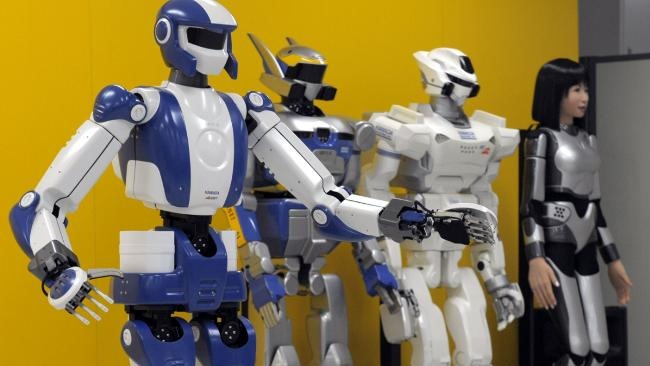
\includegraphics[width=\linewidth]{src/chap0-introduction/hrp_family.jpg}
  \end{center}
  \caption{Les robots HRP-4, HRP-2, HRP-3 et HRP-4c (de gauche à
    droite). \label{fig:hrpfamily}}
\end{figure}

Les robots humanoïdes se divisent en deux catégories: ceux de petite
taille comme le robot Nao d'Aldebaran Robotics \citep{wikipedia.nao}
et les humanoïdes de grande taille tels que ceux développés dans le
cadre du projet HRP ou bien encore par les sociétés avec le robot
Partner ou Honda avec robot Asimo. Les problématiques posées par les
deux types d'humanoïde sont assez différentes. Les robots de petite
taille utilisent des actionneurs moins puissants, de qualité moindre,
sont d'une conception moins précise par ils utilisent souvent des
squelettes en plastique plutôt qu'en métal pour des questions de
coût. Leurs capacités de calcul sont également souvent très limitées
au point qu'un ordinateur externe est souvent nécessaire pour les
commander. Les enjeux sont donc ici comment limiter les calculs
nécessaires à bord du robot étant donné les fortes contraintes sur la
capacité de calcul, comment prendre en considération les imperfections
dans la modélisation du robot, la flexibilité de ses différentes
parties ou bien encore la mauvaise précision de ses
actionneurs. L'objectif étant de fournir à moyen terme un robot
compagnon réalisant des tâches simples comme jouer avec un humain ou
fournir des services simples comme la télésurveillance. Les capacités
de manipulation de ces humanoïdes sont, à l'heure actuelle, très
limitées, voire inexisantes.


Au contraire, les grands humanoïdes sont extrêmement onéreux et
composés de pièces usinées très précisément et d'actionneurs
extrêmement performants. De ce fait, les problèmes d'identification de
modèles ne se posent qu'à la marge et le mouvement réel du robot est
très proche de sa simulation faisant l'hypothèse de mouvements de
corps rigides. Les capacités de calcul sont également plus importantes
bien qu'inférieures à ce que l'on peut trouver dans un robot mobile où
un poids important ne pose pas de problème particulier. Selon les
modèles, ces robots peuvent réaliser des tâches de manipulation
complexe. Les défis posés par ces robots sont différents: ils sont
plus lourds, plus grands et donc toute chute leur est généralement
fatale. La commande à gain fort courante sur ce type de système rend
également le comportement du système potentiellement dangereux: pour
atteindre sa consigne, le robot aura tendance à appliquer le couple
maximal de ses actionneurs, quitte à s'endommager lui-même ou à
blesser un humain se trouvant à proximité. Ils restent donc, à l'heure
actuelle, des outils de recherches dangereux impropres à une
utilisation à proximité d'humains.


\subsection{Le projet japonais HRP}


\begin{figure}
  \begin{center}
    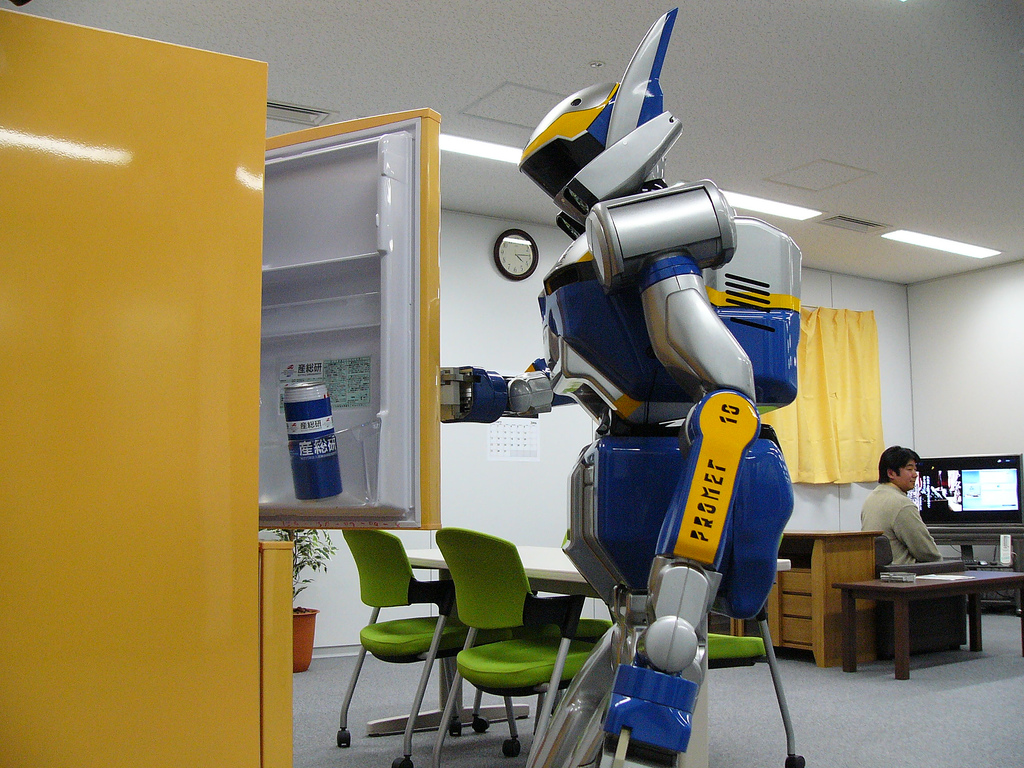
\includegraphics[width=\linewidth]{src/chap0-introduction/hrp2.jpg}
  \end{center}
  \caption{Le robot HRP-2\index{HRP-2} réalisant une tâche de
    manipulation. \label{fig:hrp2}}
\end{figure}


La totalité des recherches effectuées durant cette thèse et qui sont
décrites ici ont été validées sur la plate-forme robotique HRP-2
\citep{04kaneko.icra} du LAAS. Une version alternative est illustré
par la \autoref{fig:hrp2}. Le robot humanoïde HRP-2 ``Promet'' est un
robot humanoïde japonais mesurant 154cm et pesant 58kg. Il dispose de
deux jambes à six degrés de liberté, de deux bras à six degrés et de
deux mains à un degré de liberté commandant l'ouverture de la pince
composant chaque préhenseur. Deux degrés de liberté sont affectés au
mouvement de la tête et les deux derniers actionnent l'articulation du
torse du robot. Cette dernière étant une caractéristique unique de
cette plate-forme. Le nombre total de degrés de liberté du système est
donc de 30. Les capteurs de ce robot comprennent quatre capteurs de
force six-axes aux chevilles et au poignet, ainsi qu'une centrale
inertielle dans le torse mesurant la vitesse angulaire et
l'accélération linéaire du torse. Un système de caméras composé de
deux paires stéréo situées dans la tête est également présent. Une
première paire possède des objectifs grand-angles permettant de
percevoir une large portion de l'environnement entourant le robot
tandis que la seconde a un angle de vue plus étroit, permettant une
bonne précision lors de la manipulation. Ce robot dispose d'un système
absorbant les chocs dans chaque cheville afin de protéger la mécanique
des impacts réalisés pendant la marche. Les traitements embarqués sont
réalisés par deux ordinateurs reliés entre eux par un réseau
Ethernet. La connexion avec l'extérieur est assurée par un point
d'accès WiFi.


Ce robot conçu en 1998 a été suivi du robot HRP-3 en 2007, du robot
HRP-4C en 2009 et du robot HRP-4 en 2010. HRP-3 s'est démarqué en
étant le premier robot humanoïde résistant à l'eau ouvrant la porte à
une utilisation de ces robots en extérieur. HRP-4c est un gynoïde,
c'est-à-dire un robot humanoïde possédant l'apparence d'une femme. Les
applications ciblent le domaine du mannequinat et du divertissement
plus généralement. Le dernier robot de la série, HRP-4 est, quant à
lui, plus léger tout en conservant sept degrés de liberté pour les
bras et deux degrés de liberté pour les mains. Les différents modèles
sont illustrés par la \autoref{fig:hrpfamily}.


\section[Contributions]{Contributions, de la génération de mouvements à leur exécution}


Le maître mot de ces trois ans et demi est finalement, et cela ne peut
que se ressentir à la lecture de ce manuscrit, la polyvalence. Comme
dans toute thèse expérimentale, il a été nécessaire de tenter de
mettre en pratique des idées, de A à Z. C'est à la fois formateur et
passionnant, mais m'a conduit à utiliser de très nombreux outils,
algorithmes de l'État de l'Art et à les comprendre afin de pouvoir les
intégrer à l'approche que j'ai souhaité développer. Le travail réalisé
étant principalement de faire communiquer les idées entre elles:
comment un algorithme de vision peut-il servir la commande? Comment
les données capteur peuvent-elles être utilisées par différents
composants?  Autant de questions qui, en terme d'ingénierie
logicielle, consistent à lier des boîtes entre elles, encapsulant
autant d'algorithmes et de stratégies de décision différentes. Il est
toutefois difficile d'argumenter sur la pertinence des ``flèches''
sans expliquer au préalable ce que contiennent les ``boîtes'',
d'autant que si certaines techniques sont classiques en robotique,
d'autres sont issues des recherches du groupe GEPETTO et ne peuvent
être considérées comme allant de soi. Le choix réalisé lors de la
rédaction a donc été d'expliquer progressivement comment réaliser des
scénarii complexes avec un robot humanoïde, de la théorie, à la
pratique, mes contributions se situant davantage dans ce spectre. Le
premier chapitre de ce manuscrit traite d'un problème particulier
abordé dans le cadre de cette thèse: la représentation informatique
des problèmes d'optimisation numérique. Ce problème peut sembler
distinct de la robotique humanoïde, mais les techniques d'optimisation
sont devenues un socle supportant tant d'algorithmes utiles qu'on ne
peut pas éluder la question de la représentation de ces
problèmes. L'objectif ici est de s'appuyer sur les caractéristiques
des langages de programmation modernes, tel que le C++ afin de pouvoir
définir un problème d'optimisation une fois puis de pouvoir le
transmettre à différents solveurs de façon transparente. Une
application robotique simple valide cette approche, mais la
contribution majeure reste la formulation et la modélisation
informatique du problème. Le second chapitre explique pas à pas les
techniques de génération de mouvement et d'exécution sur le robot. Ces
techniques font partie de l'État de l'Art et il n'y a pas d'apport
original à ce niveau. Cependant, le contrôleur construit sur ces
techniques et permettant de suivre des trajectoires tout en
incorporant les données capteur est un travail totalement original et
sur lequel, à notre connaissance, aucun article antérieur n'a été
publié. Le troisième chapitre est divisé en deux: tout d'abord la
description informatique d'une pile de tâches asservie est un apport
original. La suite du chapitre est dédiée à la localisation utilisant
la vision sur un robot humanoïde. Cette partie n'est pas nouvelle en
soi, car des résultats similaires ont déjà été publiés dans ce
domaine, mais l'intégration de la localisation au schéma de contrôle
proposé dans le \autoref{chap:suivi} est un travail original. Le
dernier chapitre traite de l'intégration des différents composants sur
notre plate-forme robotique. Dans ce chapitre, la totalité des
algorithmes proposés font, soit partie de l'État de l'Art, soit ont été
conçus par d'autres équipes partenaires du LAAS, notamment l'équipe
\mbox{LAGADIC} de l'IRISA à Rennes. L'apport original de cette partie
consiste à démontrer comment on peut construire une architecture
robotique complète en utilisant des algorithmes existant afin
d'atteindre des comportements de plus haut niveau.

\chapter{Path Optimization for Humanoid Walk Planning: an Efficient Approach}
\label{chap:path-optim}

This chapter deals with path optimization for humanoid walk planning
in cluttered environments. Under the assumption that the humanoid
robot will walk on a flat floor in a perfectly modeled static
environment, it presents a heuristic and efficient optimization method
that takes as input a path computed for the humanoid bounding box, and
produces a path where a discrete set of configurations is reoriented
using an A$^{*}$ search algorithm. A pattern generator is then used to
generate a trajectory that is realistic and time-optimal. This method
is validated in various scenarios on the humanoid robot HRP-2.

\section{Motion Planning in the Configuration Space}
\label{sec:chap1-motion-planning}

The problem of motion planning is now well formalized in robotics and
several books present the various approaches
\cite{lato91,chos05,lava06}. One particularly useful concept is the
one of configuration space (denoted by \cspace) \cite{loza83}, which
is the set of all configurations \config{} of a robot \robot;
\config{} is a vector comprised of the $n$ independent degrees of
freedom (DoF) that are sufficient to know the full state of the robot
at each instant. \cspace defines then a submanifold of \espace. Some
of the robot body positions can generate (self-)collisions; the
equivalent configurations will be said to be in collision, and the set
of all configurations in collision is denoted by \cobs
$\subset$ \cspace. Its complementary is denoted by \cfree and is
called the free configuration space. Using these notations, we can
redefine the motion planning problem as the answer to the following
question: is there a continuous path $P: [0,1] \rightarrow$ \cfree
that connects a start configuration \config{s} to a goal configuration
\config{g}, and what is it?

\subsection{Deterministic Algorithms}
\label{subsec:chap1-deterministic algorithms}

This question can be answered through the use of deterministic
algorithms; for a given number of tries, they will always compute the
same valid path $P$.

FIXME: not precise
One class of algorithms, mainly developed in the past 30 years, relies
on representing \cobs explicitly in order to build a graph, also
called roadmap, that represents the connectivity of \cfree. Solving
the motion planning problem then boils down to a graph exploration to
connect \config{s} to \config{g}. A non-exhaustive list of these
methods includes cellular decomposition, Voronoi diagrams, visibility
graphs, and Canny's algorithm \cite{good04}.

Such algorithms offer the nice property of completeness, i.e. they can
always give a full answer to the motion planning problem as defined
previously. But while they work well for solving path planning
problems in low-dimensional configuration spaces, their computational
cost becomes penalizing in high-dimensional configuration spaces. In
fact building \cfree requires finding its frontiers, and computation
time is at best exponential with respect to the dimension of \cspace.

Other approaches are inspired from real-time motion generation
techniques, such as the one detailed in \cite{khat85}, which consists
in assigning artificial attractive potentials on the goals, and
repulsive ones around the start configuration and the obstacles. The
robot is then subject to forces that will direct it from the start
configuration towards the goal configuration. However, because of the
locality of the planner, a path may be computed while not being a
solution to the path planning problem. This can happen in a maze-like
environment when a stable equilibrium point other than the goal
configuration is found (see Figure
\ref{fig:chap1-deterministic-algorithm}).

\begin{figure}
  \centering
      {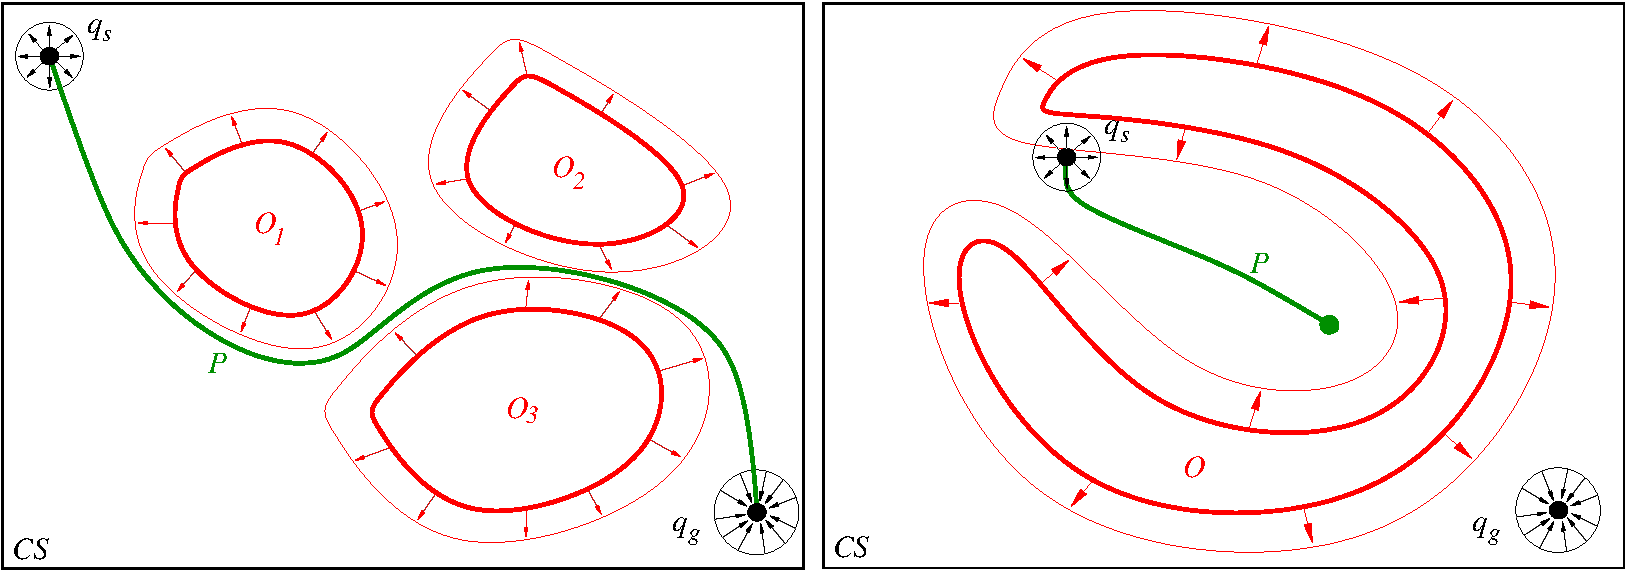
\includegraphics[width = \linewidth]
        {src/chap1-path-optimization/deterministic-algorithm.pdf}}
      \caption{Left: A valid path is computed by the deterministic
        algorithm. Arrows show the attractive and repulsive potential
        fields. Thin lines show the potential lines. Right: Example of
        problem where the stable local minimum does not coincide with
        the goal configuration. $P$ is thus not a solution to the path
        planning problem.}
      \label{fig:chap1-deterministic-algorithm}
\end{figure}

\subsection{Sampling-based Algorithms}
\label{subsec:chap1-sampling-algorithms}

Deterministic algorithms rapidly reach their limit when the
configuration space dimension rises above 4. Computation speed plays a
big part in choosing which algorithm to use for path planning
problems, as many applications require, or at least aim for, real-time
resolution. In this perspective, sampling-based algorithms, such as
Probabilistic Roadmaps (PRM) \cite{kavr96} or Rapidly-exploring Random
Trees (RRT) \cite{kuff00}, were developed in the past fifteen years.

Instead of trying to build an explicit representation of \cfree,
sampling-based algorithms rely on approximating the connectivity of
\cfree through rejection sampling: random configurations \config{rand}
are sampled in \cspace, and efficient Boolean collision detection
techniques \cite{huds97, gott96} reject configurations that produce
collisions, keeping only configurations \config{} $\in$ \cfree.

The classic RRT algorithm, as presented in \cite{kuff00}, relies on
the Voronoi bias to efficiently explore \cfree and grow a random tree
in it. Each iteration of the algorithm attempts to extend the tree by
adding new vertices in the direction of a randomly selected
configuration \config{rand}. Algorithm~\ref{alg:chap1-rrt} shows the
pseudo-code of the RRT algorithm. It takes as input an initial
configuration \config{s} and grows a tree \ctree rooted in \config{s}.

\begin{algorithm}
\caption{RRT(\config{s})}
\label{alg:chap1-rrt}
\begin{algorithmic}
\STATE \ctree$.$Init$($\config{s}$)$
\FOR{$i$ = 1 to $K$}
\STATE \config{rand} $ \leftarrow $ Rand$($\cspace$)$
\STATE \config{near}$ \leftarrow $ Nearest$($\config{rand}$,$\ctree$)$
\STATE Extend$($\ctree$,$\config{near}$,$\config{rand}$)$
\ENDFOR
\end{algorithmic}
\end{algorithm}

One way to make the RRT algorithm more efficient is to grow trees from
both the initial and goal configurations, see Figure
\ref{fig:chap1-rrt}. This was first proposed in \cite{kuff00}.

\begin{figure}
  \centering
      {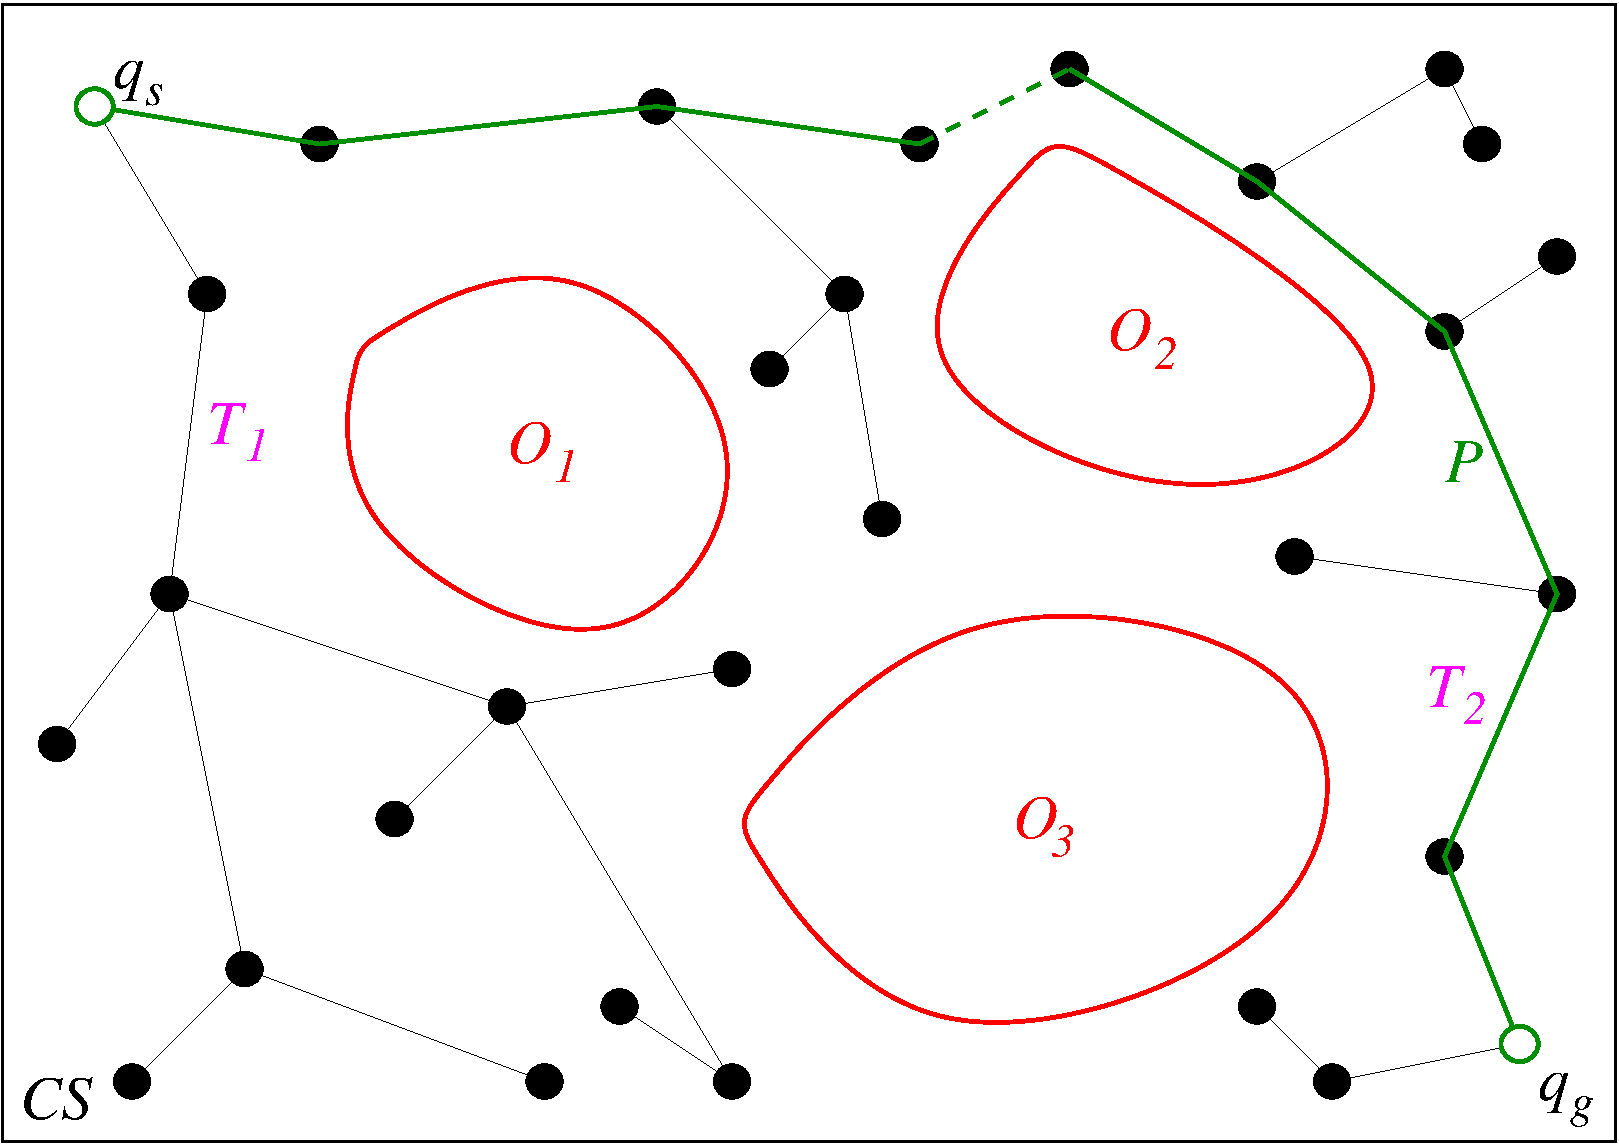
\includegraphics[width = 0.8\linewidth]
        {src/chap1-path-optimization/rrt.pdf}}
      \caption{A valid path (in green) computed with a bidirectional
        RRT planner. $q_{start}$ and $q_{goal}$ are the roots of the
        trees $\mathcal{T}_{1}$and $\mathcal{T}_{2}$ respectively. The
        algorithm keeps diffusing both trees until they can be
        connected together with an edge (in dashed green).}
      \label{fig:chap1-rrt}
\end{figure}

While not being resolution complete (i.e. they cannot tell whether a
solution exists or not), sampling-based algorithms have the less
strong property of probabilistic completeness: if a solution path
exists, the algorithm will be able to compute it with a probability of
$1$ when the number of iterations $K$ reaches infinity. This may seem
like a very weak property, but in practice these algorithms can
compute paths in complex real-life environments in a reasonable time
on regular computers and have been used to solve problems for various
systems, ranging from 6-DoF floating objects, 50-DoF anthropomorphic
systems, to 1000-DoF proteins.

\subsection{Path Optimization}
\label{subsec:chap1-path-optimization}

As shown in Figure \ref{fig:chap1-rrt}, RRT returns the shortest path
$P$ inside the graph that connects \config{s} to \config{g}. Due to
the probabilistic nature of RRT, it is clear that $P$ is not optimal
in terms of length. Path optimization methods take a valid,
i.e. collision-free, path as input and try to shorten while making
sure that the output path is still valid.

\subsubsection{Greedy Optimization}

A greedy optimizer, such as the one shown in Figure
\ref{fig:chap1-optimizers}, uses the greedy approach to shorten and
smooth a path. First, it tries to connect directly \config{s} to
\config{g}; if the path is collision-free, it tries to connect
\config{s} to the node preceding \config{g}, and so on until it
reaches \config{s}. This process is then restarted similarly on the
following nodes.

\subsubsection{Random Optimization}
\label{subsubsec:chap3-random-optimization}

In the case of the greedy optimizer, the nodes that are in the
optimized path are also nodes of the input path. Random Optimization
(RO) tries to bypass some nodes and keeps the rest. While this simple
method runs very fast, it does not always give the best possible
path. A different shortcut strategy can be run in a loop: at each
iteration, two random configurations are sampled on the path, and the
optimizer tries to connect \config{s} to the first, the first one to
the second one, and the second one to \config{g}. The local paths that
are still collision-free are then kept to make a shorter path, as
shown in Figure \ref{fig:chap1-optimizers}.

\begin{figure}
  \centering
      {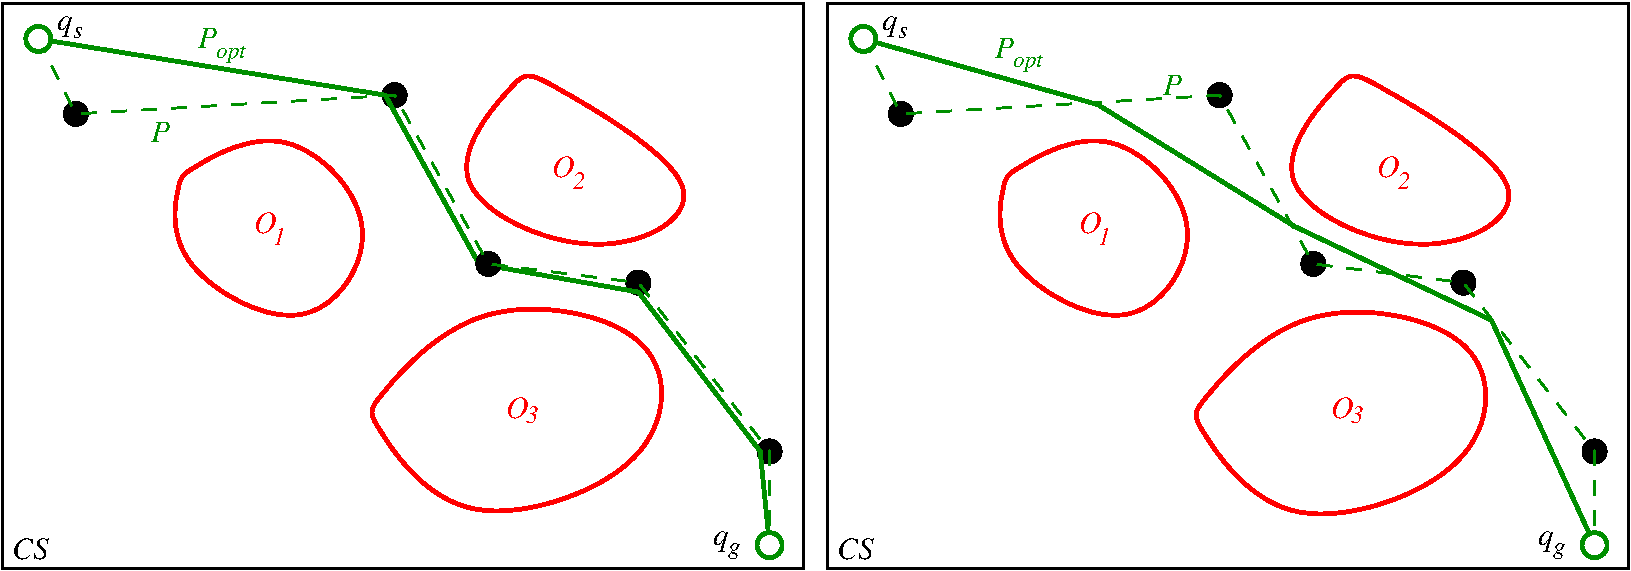
\includegraphics[width = \linewidth]
        {src/chap1-path-optimization/optimizers.pdf}}
      \caption{Left: The path $P$ (in dashed green) is optimized with
        a greedy optimizer. Right: The optimized path $P_{opt}$ (in
        continuous green) after several iterations of random
        optimization (RO).}
      \label{fig:chap1-optimizers}
\end{figure}

\section{Anthropomorphic Systems}
\label{sec:chap1-anthropomorphic-systems}

We focus in this work on humanoid robots and digital actors, which are
anthropomorphic systems. Such systems have a high number of DoF, and
are capable of accomplishing human-like tasks: locomotion(such as
walking, running and parkour), manipulation, or both. These tasks can
be accomplished thanks to the fact that anthropomorphic systems are
both underactuated and highly-redundant.

In the remainder of this work, we will refer indistinguishably to
anthropomorphic systems, humanoid robots and digital actors.

\subsection{Underactuated Systems}
\label{subsec:chap1-underactuated-systems}

A robot \robot usually composed of a set of rigid bodies \body{i}, $i
\in 0..N_B$, and a set of joints \joint{i}, $i \in 1..N_J$, which
constrain the body positions. A rigid body has a mass, an inertia, and
a given geometry. We use the kinematic tree formalism proposed in
\cite{feat08} to model a full robot: a node of the tree represents a
body of the robot, while an arc (or edge) represents a joint \joint{i}
of the robot which constrains the motion of the successor body
\body{i} with respect to its parent body \body{\lambda_{i}} (see
Figure \ref{fig:chap1-robot-kinematic-tree}). Note that in the tree
representation, each body has one and exactly one parent body, except
for the root body which has no parents; this means that additional
constraints have to be added later on in order to correctly model
robots with closed kinematic chains such as parallel robots.

\begin{figure}
  \centering
      {\def\svgwidth{0.8\linewidth}
        \subimport*{src/chap1-path-optimization/}
                   {robot-kinematic-tree.pdf_tex}}
      \caption{Left: schematic view of a humanoid robot: bodies
        are connected with joints (yellow circles) which represent the
        actuators. A fictitious 6-DoF joint, or floating joint (purple
        circle), is added to move the robot in \segroup. Right: A
        kinematic tree view of the same robot, where bodies and joints
        are represented by nodes and joints respectively.}
      \label{fig:chap1-robot-kinematic-tree}
\end{figure}

Joints usually correspond to the actuators on the physical robot. Each
type of actuator will then have an equivalent type of joint
(prismatic, revolute, etc). A configuration \config{} of such a robot
can then be defined as the concatenation of all joint DoF values, and
the set of all configurations is called the actuated configuration
space \actcspace. This is however not sufficient in the particular
case of anthropomorphic systems, which rely on making and breaking
contact with their environment -- the floor for instance -- in order
to move in their workspace. Additional information in the
configuration vector is needed to model the general position of the
system, and not only its actuators. Anthropomorphic systems are
therefore said to be unactuated systems.

We therefore introduce a 6-DoF floating joint, which we attach to the
root of the existing kinematic tree containing the actuated
joints. The successor body of the floating joint will be called the
floating base. Note that any body of the kinematic tree can be chosen
to be the floating base; in Figure
\ref{fig:chap1-robot-kinematic-tree}, the floating base is the
``waist'' of the robot. Thus, a full configuration \config{} of the
robot \robot is an element of the configuration space \cspace $=$
\segroup $\times$ \actcspace.
 
\subsection{Kinematic Redundancy}
\label{subsec:chap1-kinematic-redundancy}

\begin{figure}
  \centering
      {\def\svgwidth{0.8\linewidth}
        \subimport*{src/chap1-path-optimization/}
                   {robot-redundancy.pdf_tex}}
      \caption{Anthropomorphic systems are highly-redundant
        systems. For a desired Cartesian position (in blue) of the end
        effector \body{e}, there exists more than one configuration
        \config{} that accomplishes this task. Left and right: two
        possible solution configurations.}
      \label{fig:chap1-robot-redundancy}
\end{figure}

We briefly introduce here the concept of kinematic redundancy. Figure
\ref{fig:chap1-robot-redundancy} shows that for a same target
Cartesian position of the end effector \body{e}, there exists more
than one configuration of \robot that allows \body{e} to reach the
target. The robot \robot is therefore kinematically redundant with
respect to the task of reaching the object. One could imagine
assigning multiple tasks to be accomplished at the same time, or even
exploring \cspace while continuously accomplishing one or more
tasks. This will be discussed in more thoroughly in Chapter
\ref{chap:wholebody-planning}.

\section{Walk Pattern Generation}
\label{sec:chap1-pattern-generator}

An important field of humanoid robotics research is the generation of
dynamically balanced walk patterns. Since the introduction of the
Zero-Moment Point (ZMP) \cite{vukobratovic1969contribution}, several
methods have been proposed to generate walking motions efficiently.

\subsection{Zero-Moment Point (ZMP)}
\label{subsec:chap1-zmp}

We assume here that the robot \robot is walking on a flat horizontal
floor. We also assume that the robot is always making contact with the
floor, i.e. that there are no jumps, and that all contacts are
non-sliding. \robot is then subject to its weight and to contact
forces.

Under these assumptions, \cite{vukobratovic1969contribution} define
the Zero-Moment Point (ZMP) as the point on the floor where the
horizontal components of the sum of moments applied to \robot are
zero. It is also established that \robot will not tilt around its foot
edges as long as the ZMP lies inside the support polygon, i.e. the
convex hull of all contact points, which are coplanar due to the
previous assumptions. This is known as the condition of dynamic
balance, and the robot \robot is then said to be dynamically
balanced. We will discuss more the complete ZMP formulation in Chapter
\ref{chap:optimal-motion-planning}.

Note that in the particular case where speed and acceleration are
zero, the ZMP will coincide with the CoM vertical projection on the
floor; the robot \robot will then be said to be statically balanced if
this projection lies inside the support polygon.

\subsection{Cart-Table Model}
\label{subsec:chap1-cart-table}

The above formulation of ZMP is rather hard to control.  One way to
deal with the complexity of a humanoid robot kinematic tree is to use
the so-called "cart-table" simplified model, where the walking robot
is modeled by a point mass at a fixed height.  The equations giving
the ZMP horizontal coordinates $(p_x,p_y)$ as functions of the center
of mass (CoM) horizontal coordinates $(x,y)$ in the cart-table model
were presented in \cite{kaji03}:
\begin{equation}
\label{eq:chap1-walk-zmp}
\left(
\begin{array}{c}
p_x\\ p_y
\end{array}
\right) = \displaystyle \left(
\begin{array}{c}
x - \frac{z_c}{g} \ddot{x}\\ y - \frac{z_c}{g} \ddot{y}
\end{array}
\right)
\end{equation}
where $z_c$ is the constant height of the CoM and $g$ is the gravity
constant.

\begin{figure}
  \centering
      {\def\svgwidth{0.5\linewidth}
        \subimport*{src/chap1-path-optimization/}
                   {robot-cart-table.pdf_tex}}
      \caption{Simplified model of a cart on table. The cart can move
        horizontally along one dimension on the table with a non-zero
        acceleration and represents the robot CoM. The table foot
        represents the contact surface of the robot. Note that in its
        current state, the robot is dynamically balanced, as the ZMP
        lies on the table foot. The CoM vertical projection, on the
        other hand, doe not, and static balance is not ensured.}
      \label{fig:chap1-robot-cart-table}
\end{figure}

Based on this model, planning a trajectory for the ZMP is reduced to
planning a trajectory for CoM of the robot. Given a trajectory of the
CoM and footprint positions, inverse kinematics solvers can animate
the whole set of DoF of the robot to generate a dynamically balanced
walk trajectory.

\begin{figure}
  \centering
  \definecolor{c8eff88}{RGB}{142,255,136}
\definecolor{cffc925}{RGB}{255,201,37}
\definecolor{cff5663}{RGB}{255,86,99}
\definecolor{c454545}{RGB}{69,69,69}
\definecolor{c0200d1}{RGB}{2,0,209}

\begin{tikzpicture}[y=2.pt, x=2.pt,yscale=-1, inner sep=0pt, outer sep=0pt]
  %Start and end configurations
  \begin{scope}[cm={{0.0,1.0,-1.0,0.0,(360.33128,174.24827)}}]
    \path[draw=black,fill=c8eff88,miter limit=4.00,line width=0.800pt,rounded
      corners=0.0000cm] (47.0740,258.0597) rectangle (81.6792,276.2132);
    \path[draw=black,fill=c8eff88,line join=miter,line cap=butt,line width=0.800pt]
    (64.1273,257.7760) -- (64.1273,246.9973);
    \path[draw=black,fill=c8eff88,line join=miter,line cap=butt,line width=0.800pt]
    (64.1273,246.4300) -- (67.6730,250.2593) -- (60.8654,250.2593) -- cycle;
  \end{scope}
  \begin{scope}[cm={{0.0,1.0,-1.0,0.0,(478.33128,174.24827)}}]
    \path[draw=black,fill=c8eff88,miter limit=4.00,line width=0.800pt,rounded
      corners=0.0000cm] (47.0740,258.0597) rectangle (81.6792,276.2132);
    \path[draw=black,fill=c8eff88,line join=miter,line cap=butt,line width=0.800pt]
    (64.1273,257.7760) -- (64.1273,246.9973);
    \path[draw=black,fill=c8eff88,line join=miter,line cap=butt,line width=0.800pt]
    (64.1273,246.4300) -- (67.6730,250.2593) -- (60.8654,250.2593) -- cycle;
  \end{scope}
  %Footprints
    \path[cm={{0.0,1.0,-1.0,0.0,(0.0,0.0)}},draw=black,fill=cffc925,miter
      limit=4.00,line width=0.800pt,rounded corners=0.0000cm] (225.3161,-100.2912)
    rectangle (235.2439,-86.1087);
    \path[cm={{0.0,1.0,-1.0,0.0,(0.0,0.0)}},draw=black,fill=cffc925,miter
      limit=4.00,line width=0.800pt,rounded corners=0.0000cm] (225.3161,-144.2911)
    rectangle (235.2439,-130.1087);
    \path[cm={{0.0,1.0,-1.0,0.0,(0.0,0.0)}},draw=black,fill=cffc925,miter
      limit=4.00,line width=0.800pt,rounded corners=0.0000cm] (225.3161,-174.2911)
    rectangle (235.2439,-160.1087);
    \path[cm={{0.0,1.0,-1.0,0.0,(0.0,0.0)}},draw=black,fill=cffc925,miter
      limit=4.00,line width=0.800pt,rounded corners=0.0000cm] (225.3161,-202.2911)
    rectangle (235.2439,-188.1087);
    \path[cm={{0.0,1.0,-1.0,0.0,(0.0,0.0)}},draw=black,fill=cffc925,miter
      limit=4.00,line width=0.800pt,rounded corners=0.0000cm] (225.3161,-218.2911)
    rectangle (235.2439,-204.1087);
    \path[cm={{0.0,1.0,-1.0,0.0,(0.0,0.0)}},draw=black,fill=cff5663,miter
      limit=4.00,line width=0.800pt,rounded corners=0.0000cm] (242.4480,-100.2912)
    rectangle (252.3757,-86.1087);
    \path[cm={{0.0,1.0,-1.0,0.0,(0.0,0.0)}},draw=black,fill=cff5663,miter
      limit=4.00,line width=0.800pt,rounded corners=0.0000cm] (242.6932,-130.9444)
    rectangle (252.6209,-116.7619);
    \path[cm={{0.0,1.0,-1.0,0.0,(0.0,0.0)}},draw=black,fill=cff5663,miter
      limit=4.00,line width=0.800pt,rounded corners=0.0000cm] (242.6932,-158.9444)
    rectangle (252.6209,-144.7619);
    \path[cm={{0.0,1.0,-1.0,0.0,(0.0,0.0)}},draw=black,fill=cff5663,miter
      limit=4.00,line width=0.800pt,rounded corners=0.0000cm] (242.6932,-186.9444)
    rectangle (252.6209,-172.7619);
    \path[cm={{0.0,1.0,-1.0,0.0,(0.0,0.0)}},draw=black,fill=cff5663,miter
      limit=4.00,line width=0.800pt,rounded corners=0.0000cm] (242.8937,-218.4225)
    rectangle (252.8214,-204.2401);
  %ZMP trajectory
    \path[draw=c454545,line join=miter,line cap=butt,miter limit=4.00,line
      width=0.800pt] (92.6635,239.1801) -- (92.6635,229.8536) -- (124.1530,247.9049)
    -- (137.5913,229.8536) -- (152.2329,247.9049) -- (167.2757,230.0542) --
    (180.3127,247.3032) -- (195.5561,230.2548) -- (211.8023,247.9049) --
    (211.8023,238.6787);
  %Com trajectory
    \path[draw=c0200d1,line join=miter,line cap=butt,miter limit=4.00,line
      width=0.800pt] (92.5632,239.1801) .. controls (92.3626,227.5470) and
    (108.6088,239.0798) .. (108.6088,239.0798) .. controls (123.1502,247.7044) and
    (130.9724,238.6787) .. (130.9724,238.6787) .. controls (137.3907,229.5528) and
    (145.3132,239.2804) .. (145.3132,239.2804) .. controls (152.2329,247.5038) and
    (159.7543,239.0798) .. (159.7543,239.0798) .. controls (167.4762,229.0513) and
    (173.9948,239.1801) .. (173.9948,239.1801) .. controls (180.3127,247.5038) and
    (187.6336,238.8793) .. (187.6336,238.8793) -- (187.7338,238.6787) .. controls
    (196.9601,227.8479) and (203.3783,238.7790) .. (203.3783,238.7790) .. controls
    (211.9026,248.3061) and (211.8023,238.6787) .. (211.8023,238.6787);
  %legend
    \path[opacity=0,line join=miter,line cap=butt,line width=0.800pt]
    (85,200.7535) -- (100,200.7535)
    node[opacity=0,right] {\footnotesize Desired ZMP trajectory};
    \path[draw=c454545,line join=miter,line cap=butt,line width=0.800pt]
    (85,200.7535) -- (100,200.7535)
    node[right=2] {\footnotesize Desired ZMP trajectory};
    \path[draw=c0200d1,line join=miter,line cap=butt,line width=0.800pt]
    (85,206) -- (100,206)
    node[right=2] {\footnotesize CoM trajectory};

\end{tikzpicture}

  \caption{An illustration of the walking pattern generator: a desired
    ZMP trajectory (in grey) connects footprints. During the
    single-support phase, the ZMP stays under the support foot, and
    switches feet during the double support phase. The cart-table
    model is then used to produce the corresponding CoM trajectory (in
    blue).}
  \label{fig:chap1-zmp}
\end{figure}

\section{Humanoid Walk Planning}
\label{sec:chap1-humanoid-walk-planning}

The motion planning problem is certainly a complex one in the case of
humanoid robots, which are high-DoF redundant systems that have to
verify bipedal stability constraints. Various planning strategies can
be found in literature.

\subsection{Footstep Planning}
\label{subsec:chap1-footstep-planning}

One possible way of addressing humanoid walk planning is by reasoning
on the footstep level. Works of \cite{kuff01,ches05} describe humanoid
footstep planning schemes. Starting from an initial footstep
placement, they use an A$^{*}$ graph search \cite{hart68} to explore a
discrete set of footstep transitions. The search stops when the
neighborhood of the goal footstep placement is reached. This approach
is not practical in some environments with narrow passages, and
\cite{xia09, perr11a} reduced the computational cost of footstep
planning by adapting RRT planning algorithm and efficiently exploring
the discrete footstep space. In their most recent work, \cite{perr11b,
  perr12} give an elegant proof of the equivalence between discrete
footstep planning and a continuous motion planning, which enables the
use of off-the-shelf planning algorithms such as RRT.

\subsection{Constraints-Based Motion Generation}
\label{subsec:chap1-constraints-motion-generation}

Another category relies on prioritized whole-body task planning:
kinematic redundancy is used to accomplish tasks with different orders
of priorities \cite{khat04, saab-tro-12}. Dynamic balance and obstacle
avoidance can then be defined as unilateral constraints that the
algorithm has to verify during the whole motion. The trajectory is
then generated by specifying a set of goal tasks -- which could be a
goal configuration -- and let this set act as an attractor, in a way
similar to the simpler example shown in
\ref{subsec:chap1-deterministic algorithms}. Using such as scheme,
\cite{kano09} defines a robot augmented with a sequence of footprints
and formulates the problem of locomotion planning as an optimization
problem. Such as scheme works well in the presence of simple
obstacles, but is prone to falling and local minima failing to find
solutions in more complex environments.

\subsection{Constrained Motion Planning}
\label{subsec:chap1-constrained-motion-planning}

More recently, sampling-based motion planning algorithms were adapted
to efficiently explore a constraint submanifold of \cspace. In
\cite{bret06, haus10}, this strategy is used to plan on a union of
submanifolds, where each manifold is defined by a contact limb
position and static balance constraints, producing statically balanced
locomotions for hexapods and humanoid robots on uneven
terrain. Constrained motion planning will be further discussed in
Chapter \ref{chap:wholebody-planning}, where a new dynamically-balanced locomotion
planner is introduced.

\subsection{Multi-Contact Planning}
\label{subsec-chap1-multi-contact-planning}

It is interesting to note that while collision avoidance is a
requirement in motion planning, some features of the environment can
in fact be useful to solve the problem, especially in the case of
underactuated systems. \cite{esca06, bouy12} propose a
multiple-contact-point stance planner that looks for authorized
contacts in order to help the robot reach its goal.

\subsection{Decoupled Planning}
\label{subsec:chap1-bounding-box}

Finally, Another strategy consists of dividing a high-dimensional
problem into smaller problems and solving them successively
\cite{zhan09}. The idea of dividing the problem into a two-stage
scheme is described in \cite{yosh08}: A 36-DoF humanoid robot is
reduced to a 3-DoF bounding box. Using the robot simplified model, the
PRM algorithm solves the path planning problem and generates a valid
path for the bounding box. A geometric decomposition of the path
places footsteps on it, and the walk pattern generator described in
\ref{sec:chap1-pattern-generator} finally produces the whole-body
trajectory for the robot. In \cite{moul10}, this two-stage approach is
also used; numerical optimization of the bounding box path produces a
time-optimal trajectory that is constrained by foot speed and distance
to obstacles. Optimization techniques will be discussed in detail in
Chapter \ref{chap:optimal-motion-planning}, where we describe an
optimal motion planning framework.

\subsection{Holonomic vs Nonholonomic Walking Motion}
\label{subsec:chap1-holonomic}

An important notion on humanoid walk planning is the one of holonomic
motion.
A \emph{holonomic} \emph{constraint}, is given by:
\begin{eqnarray} C(\mathbf{q}) & = & 0,
  \label{eq:chap1-holonomic_constraint}
\end{eqnarray}
with \config{} the configuration vector. When a constraint of the form
\begin{eqnarray}
  C(\mathbf{q,}\overset{.}{\mathbf{q}}) & = & 0,
\end{eqnarray}
with $\mathbf{\overset{.}{\mathbf{q}}=}\frac{d\mathbf{q}}{dt}$, cannot
be integrated into a form similar to \ref{eq:chap1-holonomic_constraint},
this constraint is called \emph{nonholonomic}.

Practically, a nonholonomic constraint implies that a device's
velocity vector cannot take an arbitrary direction. For instance, you
cannot drive a car sideways (what makes life harder for us when
parking), and therefore it has a nonholonomic constraint. On the other
hand, a spherical ball can roll in any direction, which means it has a
holonomic constraint.

So is there a particular constraint that governs human gait? Studies,
like the one described in \cite{momb10}, established a model that
presents trajectory planning as an optimization problem of a cost
function. Basically, it is shown that for small distances and small
orientation variations between the start and goal configurations,
motion obeys a holonomic constraint, and sidestepping is allowed.
However for greater distances and orientation variations, a
nonholonomic constraint rules human gait, and sidestepping is
forbidden, i.e. the human direction is always tangent to its path.
But one should note that this model is only applicable in the case of
the absence of any obstacles, and it is clear that in the presence of
narrow passages, a human would be forced to adopt holonomic motion in
order to walk sideways.

The path planning scheme in \cite{yosh08} is designed to this end; a
PRM algorithm first builds a roadmap with Dubins curves \cite{dubi57};
but such curves impose a nonholonomic constraint and narrow passages
cannot be crossed. The roadmap is therefore enriched with linear local
paths. As a result this planning scheme generates motion such that the
robot remains tangent to its path most of the time and uses
sidestepping only in narrow passages.

\section{Contribution: Regular Sampling Optimization}
\label{sec:chap1-contribution}

The work of \cite{moul10} provides a sound way for generating nice
walking trajectories, using numerical optimization to minimize the
robot walking time along the path while following speed and obstacle
distance constraints. However, after having tried this approach, we
came to the conclusion that it was too computationally expensive given
the simple nature of the robot model, with optimizations taking
several minutes even for simple environments.

While using the same two-stage approach of \cite{yosh08}, a simpler
heuristic method that generates realistic near time-optimal humanoid
trajectories is proposed. First the PRM algorithm and the Dubins local
paths are replaced with an RRT-Connect algorithm and linear local
paths. The path is then optimized by locally reorienting the robot
bounding box on a discrete set of configurations of the path. Our
heuristic gives priority to nonholonomic motion, holonomic motion is
used only to pass in narrow passages or avoid nearby obstacles, thus
generating realistic walking trajectories.

The following section presents this method and explains how it is
integrated in the motion planning scheme. Examples of different
scenarios, including a real one with the HRP-2 platform, are shown in
\autoref{sec:chap1-examples}.

\section{Optimization by Regular Sampling}
\label{sec:chap1-regular-sampling-optim}

\begin{figure}
  \centering
      {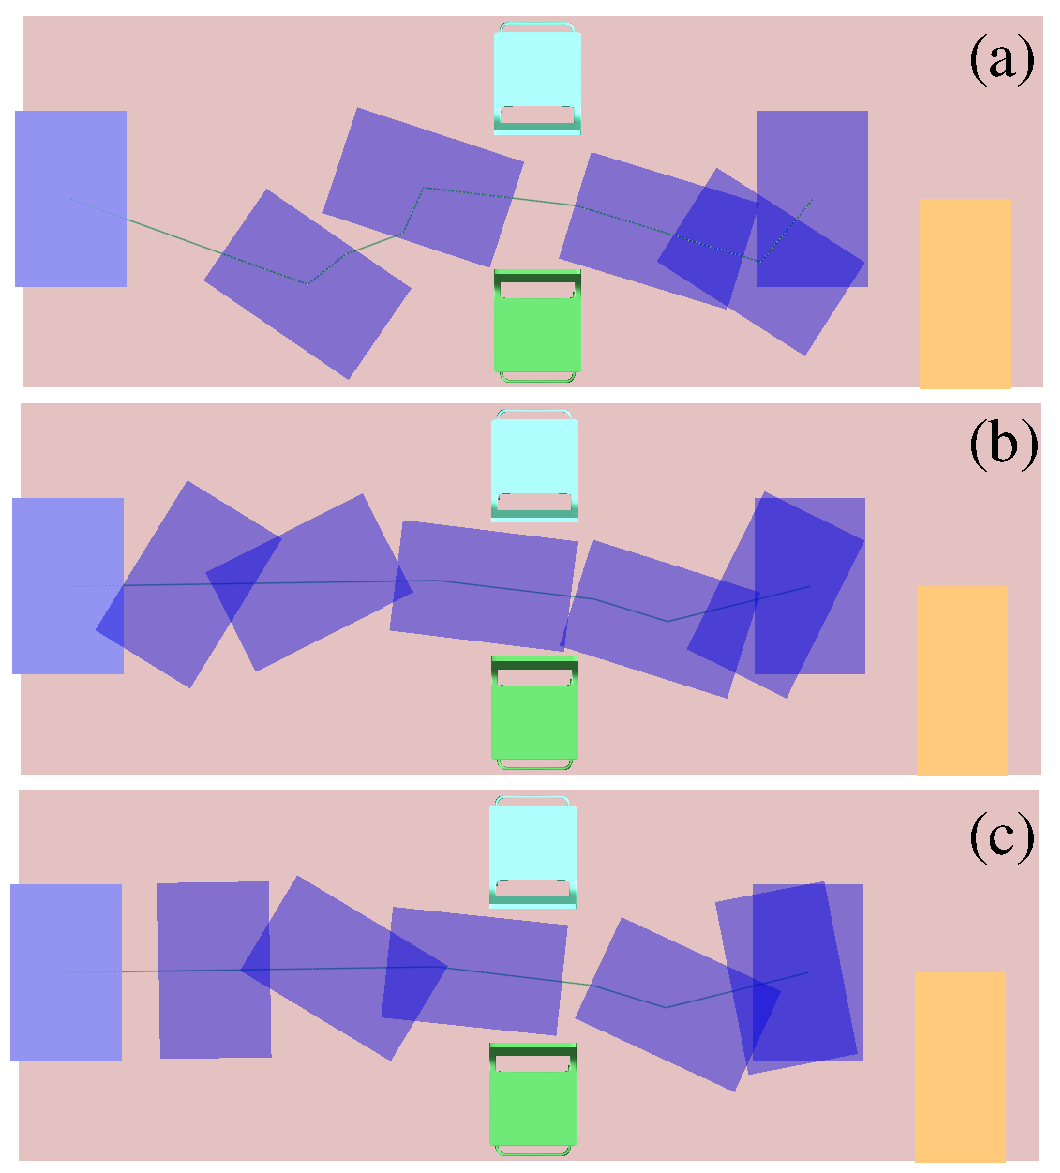
\includegraphics[width = 0.8\linewidth]
        {src/chap1-path-optimization/bb-plan-optim.pdf}}
      \caption{Top view: (a) RRT-Connect path for the bounding box
        passing between two chairs. (b) Optimized bounding box path by
        random optimization (RO). (c) Optimized bounding box after
        adding regular sampling optimization (RSO) .}
      \label{fig:chap1-bb-plan-optim}
\end{figure}

Assuming full knowledge of the environment, the RRT algorithm produces
a collision-free piecewise linear path $P_{RRT}$ for the robot
bounding box (in offline mode), i.e. the path consists of the
concatenation of linear local paths $LP_{RRT}$.

Due to the probabilistic nature of RRT, $P_{RRT}$ may not be optimal
in terms of length, and a preliminary random shortcut optimization
(RO) can be run in order to shorten it (See
\autoref{fig:chap1-bb-plan-optim}). While the optimized path $P$ is
collision-free, the bounding box orientation is such that it could
lead to an unrealistic trajectory that is not time-optimal. For
instance, the humanoid robot could spend a long time walking sideways
or backwards over a long distance in an open space. An additional
optimization stage is introduced to address this issue in the next
section.

\subsection{Bounding Box Path Optimization}
Note that each configuration \config{} can be written as $q =
(\mathbf{X},~\theta)$, where $\mathbf{X} = (x,~y)$ describes the
bounding box position in the horizontal plane, and $\theta$ gives its
orientation.  The optimizer reorients the bounding box along $P$ by
changing $\theta$ while retaining the value of $\mathbf{X}$.

For this purpose, an A$^{*}$ search algorithm is executed; first $P$ is
regularly sampled. Using a discrete set of possible orientations for
each sample configuration and an adequate heuristic estimation
function, the bounding box orientation is then modified along $P$. An
optimized path $P_{opt}$ is created and leads to a realistic
time-optimal trajectory.

\subsubsection{Preliminary Notations}
After running RO on the piecewise linear path $P_{RRT}$, the
path $P$ is also piecewise linear, and its first and last
configurations are denoted by $q_s$ and $q_g$.

Let $d_{sample} \in \mathbb{R}_+^*$ be a sampling distance. Sampling
$P$ with a distance $d_{sample}$ means dividing each local path $LP_j$
of $P$ into smaller local paths of length $d_{sample}$; each new local
path end is a sample configuration. The $n^{th}$ sample configuration
of $P$ in its initial state can be obtained by indexing new local path
ends starting from $q_s$, and is denoted by $q_n^{init}$.

\begin{figure}
  \centering
      {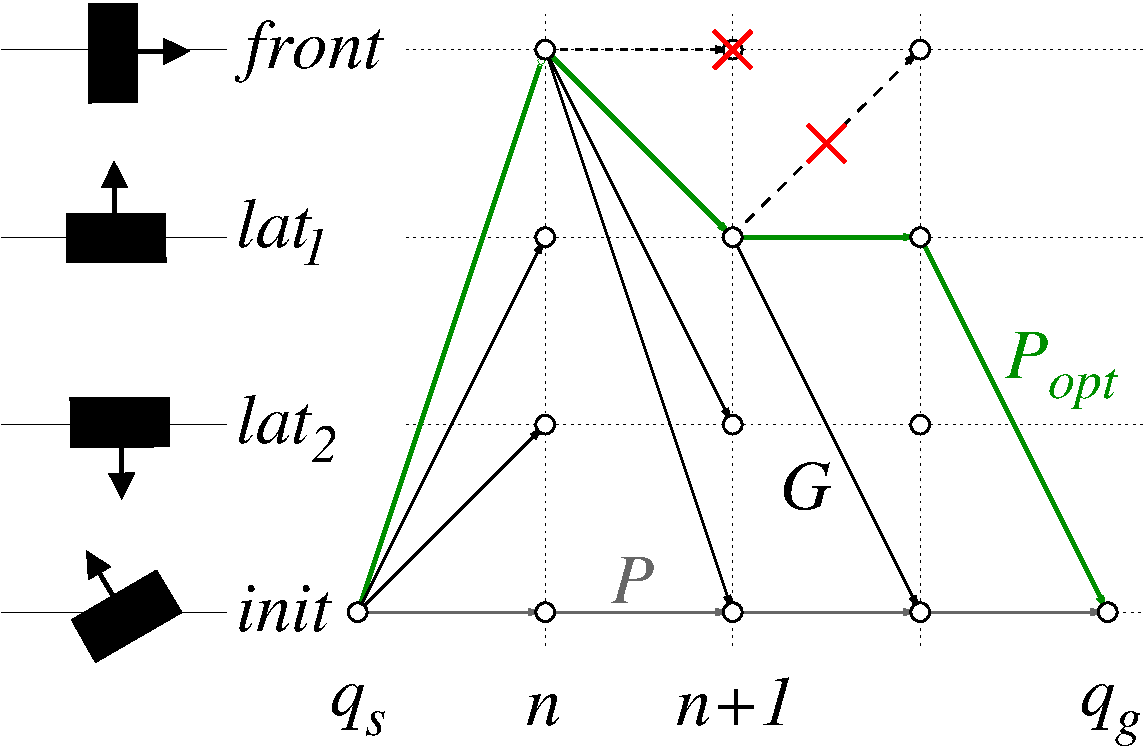
\includegraphics[width = 0.75\linewidth]
        {src/chap1-path-optimization/A-star.pdf}}
      \caption{Each initial sample configuration can be rotated and be
        in one of four states. Starting from $q_s$, the A$^{*}$ search
        algorithm searches the graph $G$ that contains only valid
        nodes and arcs to produce an optimized path $P_{opt}$.}
      \label{fig:chap1-A-star}
\end{figure}

The possible orientation states need to be defined. We aim to make a
humanoid robot reach its goal as soon as possible. Since the robot is
faster while walking straight than side-stepping, we attempt to change
the orientation of each initial sample configuration $q_n^{init}$ such
that the bounding box is tangent to the local path and introduce a new
configuration denoted by $q_n^{front}$. To take into account the fact
that there may be obstacles that forbid a frontal orientation, we also
create $q_n^{lat_1}$ and $q_n^{lat_2}$ that are rotated by
$\frac{\pi}{2}$ and $-\frac{\pi}{2}$ relative to the path tangent, see
\autoref{fig:chap1-A-star}. One particular case is local path end
configurations: the mean direction of the two adjacent local paths is
considered to define frontal and lateral configurations. This is done
to ensure a smooth transition between two local paths.

A sample configuration whose orientation is unknown will be denoted by
$q_n^{state}$. It can have any orientation state of the set
$\{init,~front,~lat_1,~lat_2\}$ except for $q_s$ and $q_g$ which
remain in their initial state.  Ideally, the algorithm should be able
(as long as there are no obstacles) to put each sample configuration
in the frontal state, create a new path $P_{opt}$ and generate a
time-optimal trajectory for the robot.

An A$^{*}$ search is run to achieve this goal; the algorithm functions are
described in the following section.

\subsubsection{A$^{*}$ Function Definition}
\label{sec:chap1-A-star}
An A$^{*}$ search algorithm can find an optimal path in a graph
as long as a graph and an evaluation function are correctly
defined. Starting from $q_s$, A$^{*}$ expands in each iteration the
possible transitions from one sample to the next one in the graph and
evaluates with the evaluation function the cost of going through each
different state, see \autoref{fig:chap1-A-star}.

A graph $G$ is defined to be a set of nodes and arcs. A valid node
$q_n^{state_n}$ is defined to be a configuration with no collisions,
and a valid arc $q_n^{state_n}q_{n+1}^{state_{n+1}}$ is a
collision-free local path. The whole graph $G$ could be built before
running A$^{*}$ by testing all nodes and arcs and making sure they are
collision-free. But collision tests are slow, and A$^{*}$ uses a heuristic
estimation function to avoid going through all nodes. An empty graph
$G$ is thus initialized and nodes and arcs are built only when
necessary. A successor operator needs to be defined for this purpose.

\begin{figure}
  \centering
      {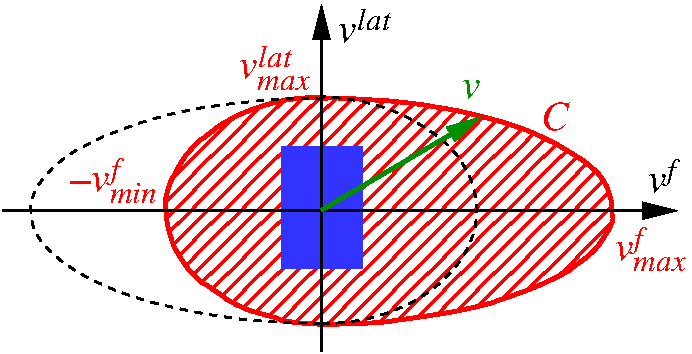
\includegraphics[width = 0.75\linewidth]
        {src/chap1-path-optimization/elliptic-constraint.pdf}}
      \caption{The rectangular bounding box speed vector $v$ is
        bounded inside the hashed area defined by the speed constraint
        $C$. The area is bounded by the union of two half-ellipsoids.}
      \label{fig:chap1-elliptic-constraint}
\end{figure}

\paragraph{The Successor operator $\Gamma(q_n^{state_n})$:}
Its value for any node $q_n^{state_n}$ is a set
$\{(q_{n+1}^{state_{n+1}},~c_{n,n+1})\}$, where
$q_{n+1}^{state_{n+1}}$ denotes a successor node, and $c_{n,n+1}$ is
the cost of going from $q_n^{state_n}$ to $q_{n+1}^{state_{n+1}}$. The
cost $c_{n,n+1}$ is defined to be the distance
$D(q_n^{state_n},~q_{n+1}^{state_{n+1}})$ between two nodes of $G$; it
computes the walk time from $q_n^{state_n}$ to
$q_{n+1}^{state_{n+1}}$. The speed constraint $C$ is defined as:
\begin{equation}
C = \left\{
\begin{array}{l l l}
  (\frac{v^{f}}{v_{max}^{f}})^2 +
  (\frac{v^{lat}}{v_{max}^{lat}})^2 - 1
  \quad \text{if } v^f >= 0 \\

  \\

  (\frac{v^{f}}{v_{min}^{f}})^2 +
  (\frac{v^{lat}}{v_{max}^{lat}})^2 - 1
  \quad \text{if } v^f < 0
\end{array} \right.
\end{equation}
where $v^{f}$ and $v^{lat}$ are respectively the frontal and lateral
speed, and $v_{min}^f$ $v_{max}^{f}$ and $v_{max}^{lat}$ their minimum
and maximum values (See
\autoref{fig:chap1-elliptic-constraint}). $D(q_n^{state_n},~q_{n+1}^{state_{n+1}})$
can be then computed by integrating this speed constraint along it.

Having expressed the successor operator, which allows the optimizer to
choose which node to expand at each iteration, the A$^{*}$ evaluation
function can be defined.

\paragraph{The Evaluation Function $\hat{f}(q_n^{state})$:}
It is the estimated cost of an optimal path going through
$q_n^{state}$ from $q_s$ to $q_g$ and can be written as:
\begin{equation}
  \hat{f}(q_n^{state}) = \hat{g}(q_n^{state}) + \hat{h}(q_n^{state})
\end{equation}
where $\hat{g}(q_n^{state})$ is the estimated cost of the optimal path
from $q_s$ to $q_n^{state}$ and $\hat{h}(q_n^{state})$ is a heuristic
function giving the estimated cost of the optimal path from
$q_n^{state}$ to $q_g$.

$\hat{h}(q_n^{state})$ must verify $\hat{h}(q_n^{state}) \leq
h(q_n^{state})$ to ensure that the algorithm is admissible, i.e. the
path from $q_s$ to $q_g$ is optimal. Since the robot is fastest while
walking straight forward in the absence of obstacles,
$\hat{h}(q_n^{state})$ is defined as:
\begin{equation}
  \begin{split}
  \hat{h}(q_n^{state}) &= D(q_n^{state},~q_{n+1}^{front}) \\
  &+ \sum_{k=1}^{N_{sample}-n-2} D(q_{n+k}^{front},~q_{n+k+1}^{front}) \\
  &+ D(q_{n+1}^{front},~q_g)
  \end{split}
\end{equation}
where $N_{sample}$ is the total number of initial sample
configurations in $P$ including $q_s$ and
$q_g$. $\hat{h}(q_n^{state})$ thus sums the cost of walking along $P$
while staying tangential to the path with the start and
end transition costs from $q_n^{state}$ and to $q_g$.

Now that the A$^{*}$ functions are fully defined, a search algorithm can be
run to compute an optimal path $P_{opt}$ by changing the orientation
of each sample node. An example is shown in
\autoref{fig:chap1-hash-direct-path}.

\begin{figure}
  \centering
      {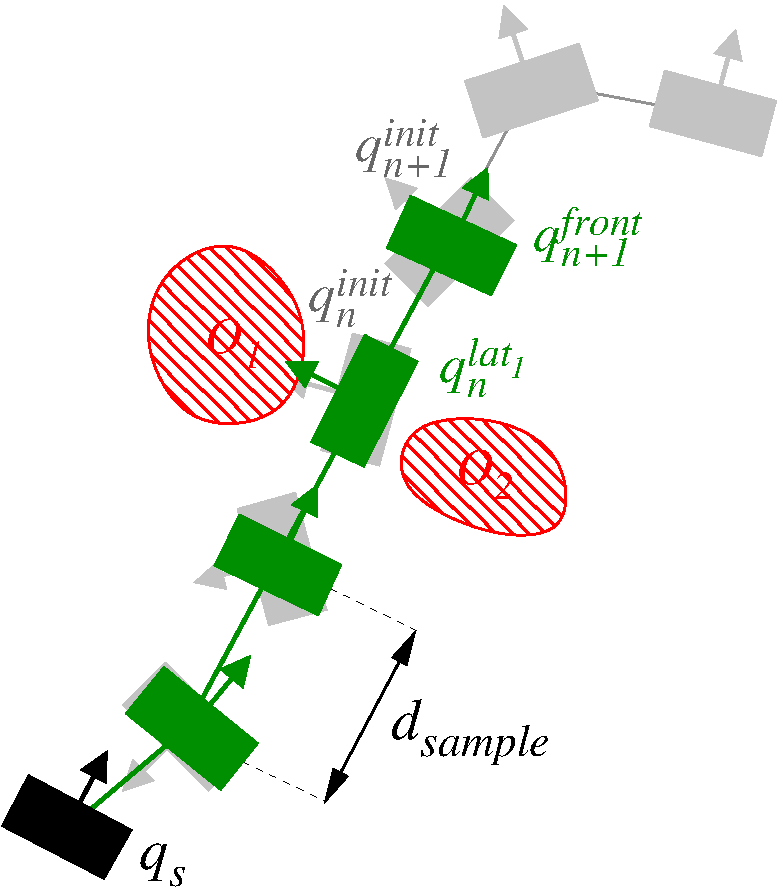
\includegraphics[width = 0.75\linewidth]
        {src/chap1-path-optimization/hash-direct-path.pdf}}
      \caption{Local paths are regularly sampled (light grey) and each
        sample configuration is reoriented (dark) while considering
        obstacles $O_1$ and $O_2$.}
      \label{fig:chap1-hash-direct-path}
\end{figure}

\subsection{Motion Generation for a Humanoid Robot}

A collision-free path $P$ for the 3-DoF bounding box can be found
using RRT-Connect and RO. The regular sampling optimization (RSO),
which is the subject of this paper, is then applied on the path and
produces a path $P_{opt}$ that gives priority to nonholonomic motion.

Once the bounding box trajectory is computed, the robot has to walk
along it. A footstep sequence is thus generated along $P_{opt}$ by
geometric decomposition of the path, and the pattern generator cited
in \autoref{sec:chap1-humanoid-walk-planning} then produces the robot
whole-body trajectory.

\section{Examples}
\label{sec:chap1-examples}

\begin{table}
\centering
\begin{tabular}{c|c|c|c|c|c|}
  \cline{2-6}
  & RRT-Connect & RO & RSO & Robot Trajectory & Total\\
  \hline
  \multicolumn{1}{|c|}{Chairs} & $3.97$ & $1.89$ & $2.14$ & $66.1$ & $74.1$\\
  \hline
  \multicolumn{1}{|c|}{Boxes} & $0.0917$ & $2.50$ & $0.238$ & $65.7$ & $68.6$\\
  \hline
  \multicolumn{1}{|c|}{Apartment} & $1.21$ & $2.43$ & $2.41$ & $223$ & $229$ \\
  \hline
\end{tabular}
\caption{Computational time (s) of each planning stage for the
  presented scenarios.}
\label{tab:chap1-computation-time}
\end{table}

\begin{table}
\centering
\begin{tabular}{c|c|c|}
  \cline{2-3}
  & RO & RO+RSO \\
  \hline
  \multicolumn{1}{|c|}{Chairs} & $40$ & $35$ \\
  \hline
  \multicolumn{1}{|c|}{Boxes} & $66$ & $57$ \\
  \hline
  \multicolumn{1}{|c|}{Apartment} & $200$ & $120$ \\
  \hline
\end{tabular}
\caption{Humanoid robot walk time (s) for the presented scenarios
  using RO alone and a RO-RSO combination.}
\label{tab:chap1-walk-time}
\end{table}

\begin{figure}
  \centering
      {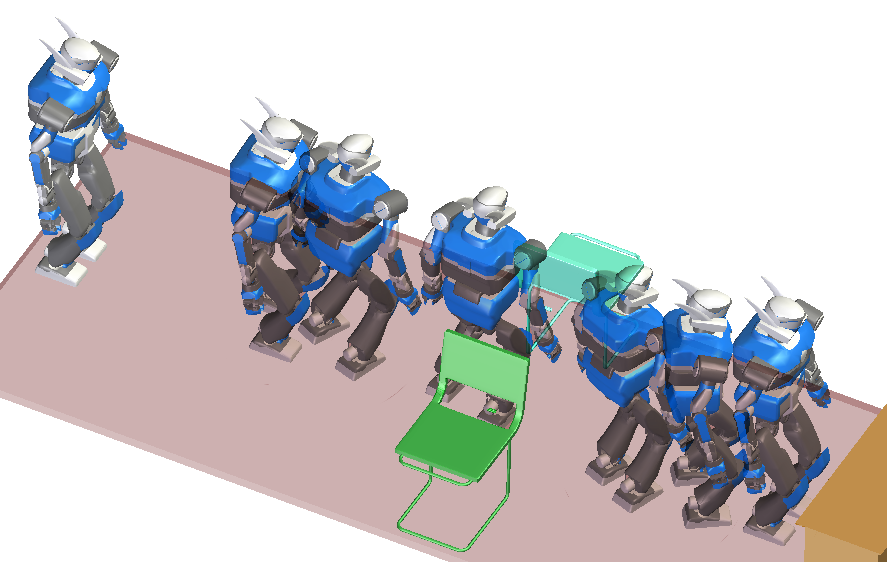
\includegraphics[width = \linewidth]
        {src/chap1-path-optimization/chairs-hash-optim-perspective-hrp2.png}}
      \caption{Perspective view of the simulated HRP-2 trajectory on
        the final optimized path passing between two chairs.}
      \label{fig:chap1-chairs-hash-optim-perspective-hrp2}
\end{figure}

This section presents experimental results of the path optimizer after
it has been inserted in the previously described walk planning
scheme. Distance parameters $v_{max}^f$, $v_{max}^{lat}$, $v_{min}^f$
are set to 0.5, 0.1, and 0.25 respectively. Note that these parameters
give an idea of the robot walking speed and play a key role in giving
priority to forward walking with respect to lateral and backwards
walking, but do not hold any physical significance, hence the absence
of units.

Since the A$^{*}$ search only takes place over the graph of discretized
configurations of the input path. It is important to choose a proper
value of the sampling interval $d_{sample}$. If the value is too
small, the search space will be much bigger, possibly leading to
better trajectories, but leading to an explosion of the A$^{*}$ search
time. If the value is too high, the A$^{*}$ search will be very fast in the
small trajectory space, but we risk missing some optimizations on the
trajectory. We found that setting $d_{sample}$ to be equal to
$\frac{h}{6}$, where $h$ is the humanoid height provided a good
comprise between computation time and trajectory quality: $d_{sample}$
is then a broad approximation of the nominal human step length.

Tests are performed on a 2.13 GHz Intel Core 2 Duo PC with 2 GB RAM.
Simulations of the humanoid robot HRP-2 are run in three scenarios.
The first one is a small environment where HRP-2 has to pass between
two chairs. The second environment is uncluttered with few obstacles
lying around, while the last one is a bigger apartment environment
where the robot has to move from one room to another while passing
through doors. The chairs scenario motion is also replayed on the real
robot HRP-2 (See Figure \ref{fig:chap1-hrp2-chairs}).

\begin{figure}
  \centering{
    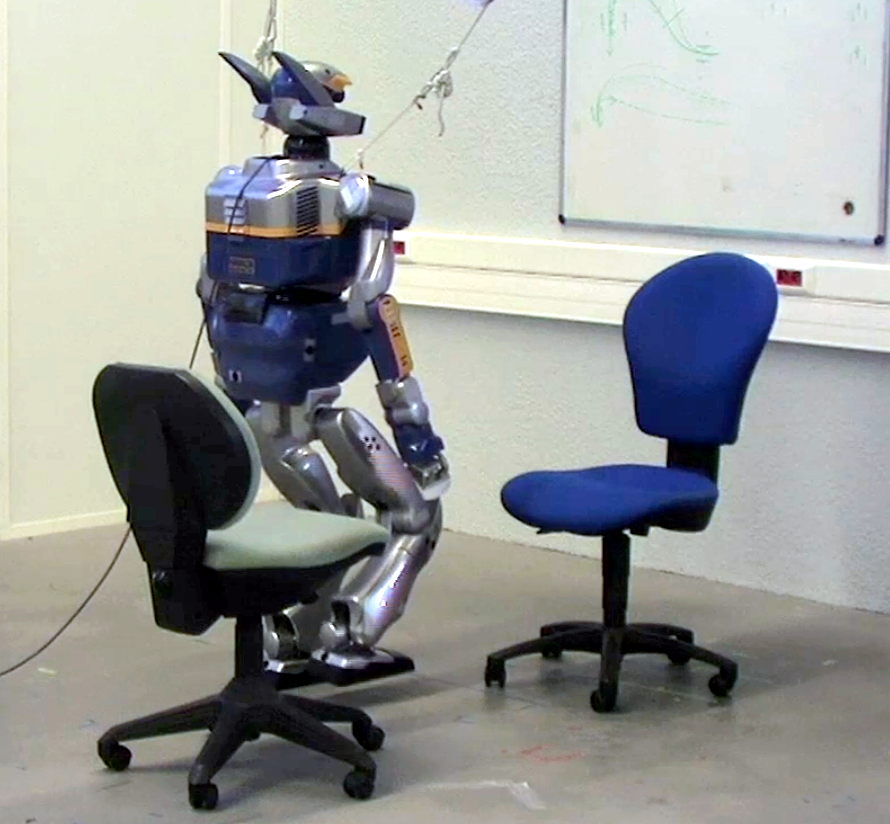
\includegraphics[width = 0.75\linewidth]
                    {src/chap1-path-optimization/hrp2-chairs.png}}
  \caption{Humanoid Robot HRP-2 uses holonomic motion, or
    side-stepping, to pass between two chairs.}
  \label{fig:chap1-hrp2-chairs}
\end{figure}

\ref{tab:chap1-computation-time} shows computation times for each
stage of the planning scheme: RRT-Connect, RO, RSO, and the whole-body
robot trajectory generation. In order to show the optimizer
contribution, robot walk times are also measured by creating a
trajectory directly after RO, and comparing it with a trajectory where
the RSO was added, see \autoref{tab:chap1-walk-time}.

\subsection{``Chairs'' Scenario}
\label{subsec:chap1-chairs}

\autoref{fig:chap1-bb-plan-optim} shows the bounding box RRT path
and the RO path for the chairs scenario. It is obvious that RO creates
a shorter path, but the bounding box starts rotating from the
beginning of the path even though the two chairs are still far. This
causes the robot trajectory to be unrealistic on one hand and, since
walking sideways takes a longer time than walking straight, to also
not be time-optimal.

\begin{figure}
  \centering
      {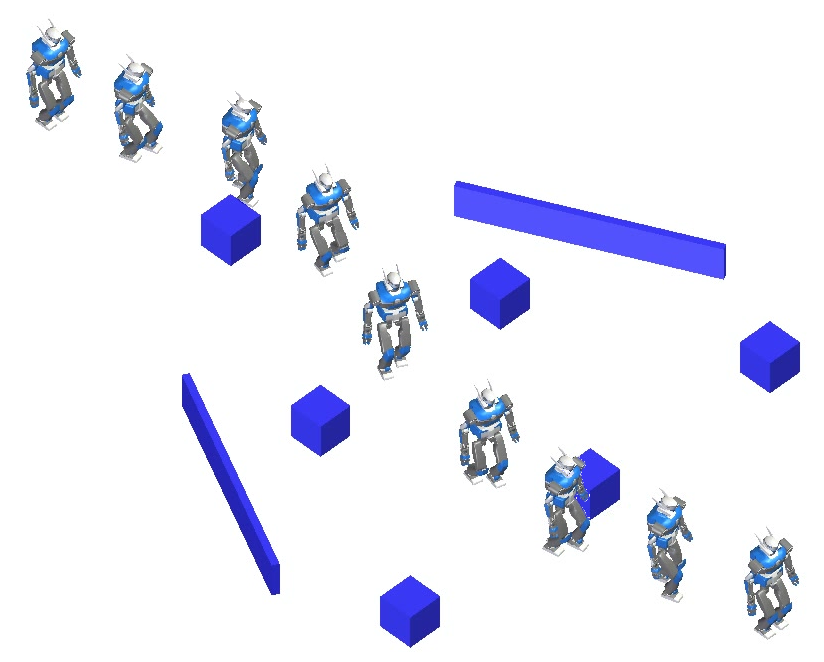
\includegraphics[width = \linewidth]
        {src/chap1-path-optimization/galton-hash-optim-perspective-hrp2.png}}
      \caption{Perspective view of HRP-2 optimized trajectory in the
        Galton board scenario.}
      \label{fig:chap1-galton-hash-optim-perspective-hrp2}
\end{figure}

However, after applying RSO, it is clear that the bounding box stays
oriented towards the front and rotates only when it reaches the
chairs. \autoref{fig:chap1-chairs-hash-optim-perspective-hrp2} and
\autoref{tab:chap1-walk-time} show that the walk time is shorter by 5
s and the final trajectory for HRP-2 is more realistic. Note that the
RSO takes 2,144 ms to be executed on the chairs path, which is less
than 3\% of the total computation time.

\subsection{``Galton'' Scenario}
An uncluttered environment is considered in this case, and
it can be seen that RRT-Connect and RSO computation times are very low
compared to other environments. This can be explained by the fact that
a tree connecting start and goal configurations is easier to find, and
that the frontal orientation state is valid for all considered samples
on the path (See \autoref{fig:chap1-galton-hash-optim-perspective-hrp2}).

\subsection{``Apartment'' Scenario}
The planning scheme is finally applied in the apartment scenario. In
\autoref{fig:chap1-apartment-hash-optim-perspective-hrp2}, it is
evident that HRP-2 walks facing forward through the doors. As with
previous scenarios, the trajectory is more realistic than a trajectory
where RSO is not used. The added computation time for RSO is 2,412 ms,
which is insignificant compared to the 228 s it takes for the whole
planning scheme.

Additionally, since the environment is significantly larger and more
constrained than the previous ones, the walk time difference is more
striking: \autoref{tab:chap1-walk-time} shows that it takes the robot
80 s less to cross the apartment when an RO-RSO combination is used.

\begin{figure}
  \centering
      {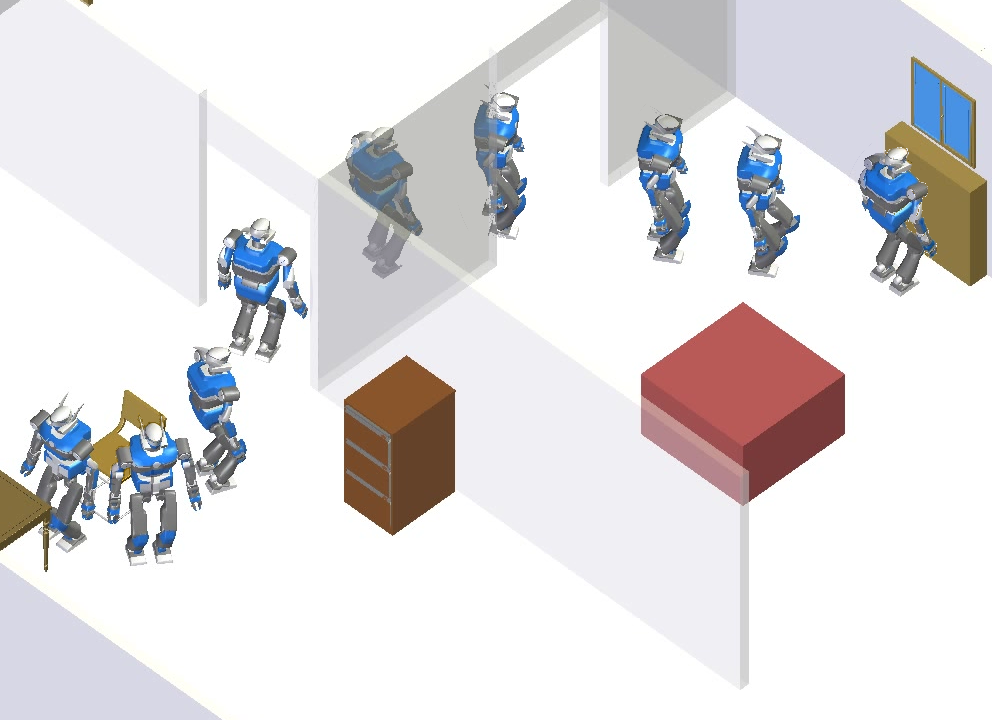
\includegraphics[width = \linewidth]
        {src/chap1-path-optimization/apartment-hash-optim-perspective-hrp2.png}}
      \caption{Perspective view of HRP-2 optimized trajectory in the
        apartment scenario.}
      \label{fig:chap1-apartment-hash-optim-perspective-hrp2}
\end{figure}

\section{Conclusion}
In this chapter, a novel simple optimization method is
presented for humanoid walk planning that relies on a decoupling
between trajectory and robot orientations. It uses an A$^{*}$ search that
takes as input a path for the robot bounding box, and produces a path
where a discrete set of configurations have been reoriented to generate
a realistic time-optimal walk trajectory. Results show that new
trajectories are more satisfactory while the added computation time is
insignificant compared to the whole planning time.

This approach can be used in other fields such as graphical animation
for digital actors to adapt the body orientation with respect to the
goal during locomotion. With a motion capture library containing
prerecorded nonholonomic and holonomic walk behaviors, it is possible
to lay this behavior on the actor trajectory and produce realistic
movements.

Achieving humanoid walk planning using the bounding box approach is
both simple and efficient; it allows using off-the shelf
sampling-based planners to efficiently explore the configurations
space, thus removing the need to take into account additional
kinematic and balance constraints when planning for the whole
articulated robot. But it has one major drawback: in order to have a
sound framework which always produces collision-free walking
trajectories, the bounding box must contain all the robot geometries
and take into account the robot swaying motion during walking. It is
thus a rather conservative method, and it might not succeed in finding
collision-free trajectories in cluttered environments. If we go back
to the chairs example in \ref{subsec:chap1-chairs}, we can show that
the lateral walking motion could have been avoided if the HRP-2 lifted
its arms over the two chairs. Besides leading to an even faster
motion, walking forward could be necessary if vision systems were
needed to achieve robot localization and/or environment mapping.

In the next chapter, we introduce a sound whole-body motion planning
algorithm that allows planning collision-free walking trajectories for
the fully articulated humanoid robot, hence releasing it from its
bounding box constraint and increasing its accessible workspace.

%\chapter{Suivi de trajectoire}
\label{chap:suivi}


FIXME: cite igor mordatch (or later on in Chapter 3 as opening?)


\epigraph{\foreignlanguage{USenglish}{I can calculate the motion of
    heavenly bodies, but not the madness of people.}}{Isaac Newton}
\clearpage

\lettrine[lines=2, lraise=0.1, nindent=0em, slope=-.5em]%
{C}{e} chapitre est dédié au problème de la génération et de
l'exécution asservie de trajectoires pour un robot humanoïde. Les
robots humanoïdes sont des robots ayant une forme anthropomorphe:
une tête, deux bras, deux jambes et un torse. La locomotion est donc
bipède et les robots humanoïdes ont la possibilité d'effectuer des
tâches dextres. De ces choix résulte un système hautement dimensionné
pour lequel il est difficile de générer des trajectoires et dont le
contrôle est délicat, l'équilibre d'un système bipède étant précaire
par nature. Au long de ce chapitre, nous verrons comment modéliser ce
système, comment représenter et calculer des mouvements pour ce
dernier afin qu'il puisse se mouvoir et réaliser différentes
tâches. Seront ensuite étudiées les différentes approches de la
littérature ainsi que leurs forces et leurs faiblesses. La troisième
section portera sur l'apport de cette thèse au problème de l'exécution
de trajectoire via la proposition d'une architecture de contrôle pour
les robots humanoïdes asservie capteur. Les résultats expérimentaux
seront ensuite détaillés pour illustrer une tâche dans laquelle le
système proposé se révèle utile. Enfin, les prospectives montreront
quelles sont les possibilités d'améliorations de l'approche proposée
et quels futurs travaux restent à réaliser.

\section{Génération de mouvements}
\subsection{Structure robotique}

Un robot est un système composé par des actionneurs -- moteurs --, des
capteurs et des unités de calcul logique -- ordinateurs -- travaillant
de concert pour constituer une entité cohérente pouvant impacter le
monde réel afin de réaliser l'objectif qui lui a été confié. En ce qui
concerne la génération de mouvements, deux éléments sont primordiaux:
d'une part les capacités motrices du système, modélisées sous la forme
d'un arbre cinématique et d'autre part sa forme dans le monde
représenté par la forme géométrique des différentes parties du
système. La forme géométrique d'un robot variant généralement sous
l'action de ses actionneurs, elle est donc conditionnée par l'état de
l'arbre cinématique\index{arbre cinématique}.

\begin{mydef}
  Un arbre cinématique\index{arbre cinématique} est un ensemble
  d'articulations\index{articulation}\index{joint|see{articulation}}
  formant un arbre. Soit $\mathcal{A}$ un arbre cinématique, on a:

  \begin{equation}
    \mathcal{A} = \emptyset \cup \{ (\mathcal{J}_0, \mathcal{C}_0),
    \dotsc, (\mathcal{J}_n, \mathcal{C}_n) \}
  \end{equation}

  Un arbre est donc, soit l'ensemble vide, soit une liste de joints
  associés à un sous-arbre. Cette définition permet de construire
  récursivement un arbre cinématique.

  À cet arbre de joints correspond une liste de joints, les joints
  sont habituellement référencés par leur ordre dans cette liste sous
  la notation $\mathcal{J}_n$ où $n$ est la position du joint dans la
  liste.
\end{mydef}

\begin{mydef}
  Le joint $\mathcal{J}_n$ modélise le mouvement du repère $n+1$ par
  rapport au repère $n$ selon un certain nombre de paramètres appelés
  degrés de liberté. Chaque joint définit implicitement son repère
  attaché. Le repère attaché à $\mathcal{J}_0$ est habituellement
  appelé repère ``monde'' et est noté $\mathcal{W}$.

  Un joint peut donc se modéliser comme une fonction:

  \begin{equation}
    \left\{
    \begin{array}{cccc}
      \mathcal{J}_n : & \mathbb{R}^m & \rightarrow & SE(3)\\
      & \mathbf{q} & \mapsto & \mathcal{J}_n(t)
    \end{array}
    \right.
  \end{equation}

  Dans l'équation le joint $\mathcal{J}_n$ possède $m$ degrés de
  liberté permettant de déterminer la transformation relative entre le
  repère $n$ et $n + 1$ qui est un élément du groupe spécial euclidien
  de dimension 3. Ces fonctions permettent donc d'exprimer des
  contraintes sur les mouvements du corps du robot au niveau des
  articulations actionnées.
\end{mydef}

Plusieurs types de joints sont habituellement utilisés en robotique,
mais nous n'allons ici en détailler que deux:
\begin{description}
\item[Joint libre -- ou joint flottant --.]\index{joint!libre} Ce joint
  comporte six degrés de liberté, soit le nombre de paramètres
  nécessaire et suffisant pour spécifier une pose dans
  $SE(3)$. Autrement dit, ce joint n'impose aucune contrainte
  particulière sur le mouvement et correspond donc à la fonction
  identité, à la représentation de la pose prête.
\item[Joint rotation.]\index{joint!rotation} Ce joint comporte un seul
  degré de liberté. Dans ce cas, la position du prochain corps du
  robot est définie par la valeur de ce degré de liberté, interprété
  comme une rotation d'un angle équivalent autour d'un axe. A chaque
  joint rotation est donc, soit associé un axe de rotation, soit un axe
  standard est choisi: par exemple, toutes les rotations seront
  réalisées autour de l'axe X.
\end{description}


Une fois cette structure construite, une attente naturelle est pouvoir
exprimer son état. C'est l'objectif du vecteur de
configuration\index{vecteur de
  configuration}\index{configuration|see{vecteur de configuration}}.

\begin{mydef}
  Soit $\mathbf{q}$ le vecteur de configuration de l'arbre cinématique
  $\mathcal{C}$. Soit $\mathcal{J}_0, \dotsc, \mathcal{J}_n$
  l'ensemble des articulations de $\mathcal{C}$. Le vecteur de
  configuration a pour dimension: $\sum_{i=0}^n \#\mathcal{J}_i$, la
  somme des arités des articulations interprétées comme fonctions,
  c'est-à-dire le nombre de degrés de liberté de toutes les
  articulations.


  Les valeurs du vecteur de configuration sont alors les valeurs des
  degrés de liberté des joints concaténés les uns aux autres selon un
  parcours de l'arbre donné. En général, le parcours main gauche de
  l'arbre est utilisé.
\end{mydef}

\begin{figure}[htbp!]
  \begin{center}
  \begin{tikzpicture}
    \Tree [ .{$\mathcal{J}_0$ (6)} [ .{$\mathcal{J}_1$ (1)} {$\mathcal{J}_2$ (2)} {$\mathcal{J}_3$ (1)} ] {$\mathcal{J}_4$ (1)} ]
  \end{tikzpicture}

  \begin{tabular}{|ccc|c|cc|c|c|}
    \hline
    $\mathcal{J}_0$ (1) & \ldots & $\mathcal{J}_0$ (6)
    & $\mathcal{J}_1$ (1) & $\mathcal{J}_2$ (1) & $\mathcal{J}_2$ (2) & $\mathcal{J}_3$ (1) & $\mathcal{J}_4$ (1)\\
    \hline
  \end{tabular}
  \end{center}

  \caption{Un exemple de chaîne cinématique et son vecteur de
    configuration correspondant. Les nombres entre parenthèses
    indiquent le nombre de degrés de liberté dans l'arbre ou le numéro
    du degré de liberté dans le joint pour le vecteur de
    configuration.}
\end{figure}

On notera que l'arbre cinématique d'un robot humanoïde est souvent
composé d'un joint libre à la racine suivie de joints rotation pour le
reste de l'arbre. À partir de maintenant, cette forme sera
systématiquement utilisée ce qui nous permettra de diviser le vecteur
de configuration en deux parties: d'un côté la position du robot dans
le plan, définie par une sous-partie des degrés de liberté du joint
libre à la racine, le repère de ce joint définissant de ce fait le
repère monde $\mathcal{W}$ et d'autre part les degrés de liberté
internes correspondant à une réalité mécanique. Sous l'hypothèse que
le robot se déplace sur un sol plan, on aura donc:

\begin{equation} \label{eq:chap2_configuration}
  \begin{aligned}
    \mathbf{x} &= [x, y, r_z]\\
    \mathbf{q} &= (\mathbf{x}, [z, r_x, r_y, \mathbf{q}_{\text{int}}])
    \in \mathcal{C} = \text{SE}(2) \times \mathcal{C}_{\text{int}}
  \end{aligned}
\end{equation}

Les six paramètres du joint racine sont: $[x, y, z, r_x, r_y, r_z]$ et
définissent une position dans l'espace 3D. Toutefois, dans la mesure
où la position du robot est contrainte par la physique, c'est-à-dire
que l'on peut raisonnablement supposer un contact planaire entre les
pieds du robot et le sol, on peut se contenter de considérer la
position du robot en deux dimensions dans le plan. Pour cette raison,
on peut considérer: $\mathbf{x} = [x, y, r_z] \in \text{SE}(2)$ pour
déterminer la position du robot dans l'espace. $\mathcal{C}$
représente alors l'espace des configurations et
$\mathcal{C}_{\text{int}}$ est l'espace des configurations
correspondant aux degrés de liberté internes uniquement. Ce découpage
peut sembler arbitraire au premier abord, mais prend son sens quand on
considère quels degrés de liberté peuvent dériver suite à des erreurs
de modélisation ou d'exécution: la position du robot dans le plan peut
se révéler fausse et doit être estimée et corrigée constamment alors
que les degrés de liberté $[z, r_x, r_y]$ ne peuvent pas subir de
dérives durant le mouvement. Le problème de la correction des erreurs
est détaillé plus loin dans ce chapitre et le problème de la
localisation d'un robot humanoïde est abordé dans le chapitre
suivant.


Une fois cette chaîne cinématique définie, on peut y attacher les
informations concernant les corps du robot, leur réalité physique:
forme et information inertielles en particulier. La forme est stockée
sous la forme d'une soupe de polygones réalisant une approximation de
la forme originale du corps du robot. Quant aux informations
inertielles, elles consistent en le poids du corps, la position de son
centre de masse et sa matrice d'inertie.


\subsection{Cinématique directe et inverse}
\index{cinématique directe}

\subsubsection{Cinématique directe}

À partir de la structure définie dans la section précédente, la
première opération que l'on souhaite réaliser est de pouvoir
déterminer la position des corps du robot en fonction de la
configuration de ce dernier. Cette opération, appelée calcul de la
géométrie directe, consiste en la fonction suivante:

\begin{equation}
  \text{GéométrieDirecte}_{\mathcal{C}}(q) = \{
  \transformation{\mathcal{W}}{\mathcal{J}_0}, \dotsc,
  \transformation{\mathcal{W}}{\mathcal{J}_n} \}
\end{equation}

La notation $\transformation{\mathcal{A}}{\mathcal{B}}$ représente la
transformation qui donne la position du repère $\mathcal{B}$ relative
au repère $\mathcal{A}$. L'intérêt de cette représentation est de
pouvoir assembler les transformations facilement, en effet, on a:

\begin{equation}
  \transformation{\mathcal{A}}{\mathcal{C}} = \transformation{\mathcal{A}}{\mathcal{B}} \transformation{\mathcal{B}}{\mathcal{C}}
\end{equation}

Les transformations géométriques sont des éléments du groupe spécial
euclidien $\text{SE}(3)$. Le produit utilisé ici est donc le produit
de groupe. Dans le cas où ces éléments sont représentés sous la forme
de matrices homogènes, le produit de groupe est le produit matriciel
usuel.


La géométrie directe donne donc la position de tous les corps dans le
repère monde. Dans la section précédente, on a défini un joint comme
la position du repère attaché au joint suivant par rapport à la
position du joint actuel.

\begin{mydef}\label{def:chap2-geomdirect}
Soit $\mathcal{J}_n$ un joint de l'arbre cinématique et $\Delta =
\{\mathcal{J}_0, \dotsc, \mathcal{J}_n\}$ le chemin dans l'arbre de la
racine au noeud $\mathcal{J}_n$. Soit $\mathbf{q}_i$ les degrés de
liberté du joint $\mathcal{J}_i$. La position du joint $\mathcal{J}_n$
dans le repère monde est:
\begin{equation}
  \transformation{\mathcal{W}}{\mathcal{F}_i} = \prod_{j \in \Delta} \mathcal{J}_j (\mathbf{q}_j)
\end{equation}
\end{mydef}


\subsubsection{Cinématique inverse}
\index{cinématique inverse}

La \autoref{def:chap2-geomdirect} permet de construire la position de
tous les corps du robot dans le repère monde attaché au joint racine
de la structure. Cependant, lors de la conception d'un problème
robotique, il est courant de vouloir, par exemple, positionner un
effecteur du robot -- un préhenseur par exemple -- à un endroit
particulier de l'espace euclidien. Dans ce cas, le problème inverse
doit être résolu: trouver une configuration telle qu'un corps
particulier du robot atteigne une position donnée. Ce problème est
appelé géométrie inverse.


Une difficulté de ce problème est que l'on doit inverser une équation
dont le nombre de variables correspond au nombre de degrés de liberté
du robot et dépend évidemment de sa structure. Si l'on souhaite
positionner un corps à un endroit précis en rotation et translation,
six variables sont nécessaires. De ce fait, selon le nombre de degrés
de liberté du système et la position à atteindre, aucune solution, un
nombre fini ou infini de solutions peuvent exister. La résolution
analytique n'étant pas toujours possible, les outils numériques ont
montré leur capacité à résoudre efficacement ce problème.

%Une technique de résolution
%possible sera détaillée dans la section FIXME.

%FIXME: vitesse des corps

\subsection{Mouvements dynamiques d'un corps dans l'espace}

La cinématique directe permet de calculer la vitesse de corps dans
l'espace indépendamment de leur réalité physique. Cependant, ce n'est
pas suffisant pour pouvoir générer un mouvement complexe: le poids des
corps du robot, leurs propriétés inertielles ainsi que les forces
exercées s'appliquant au robot doivent être prises en compte pour
pouvoir donner un mouvement qui n'est pas seulement viable dans un
monde sans physique, mais également dans le monde réel où les lois de
la physique s'appliquent.

Pour ce faire, nous allons commencer par rappeler les notions de
mécanique nécessaires à la génération de mouvements et les différents
modèles simplifiés utilisés en robotique humanoïde. Tout l'enjeu de la
robotique humanoïde se joue ici: d'un côté on ne peut ignorer la
physique pour générer un mouvement de marche, mais de l'autre le coût
important de la résolution des modèles de la physique classique
newtonienne empêche l'écriture de contrôleurs suffisamment rapides
pour pouvoir fonctionner en temps réel sur un robot. Il y a ici un
compromis à trouver qui fait toute la richesse de la robotique
humanoïde: quelles simplifications adopter? quels calculs peuvent être
réalisés à l'avance, une fois pour toutes, et quels calculs doivent
être évalués en ligne? Nous allons tout d'abord nous attacher à
rappeler les lois de la mécanique classique avant de nous intéresser
aux différentes simplifications qui permettent de rendre le problème
tractable.


\subsubsection{Quelques éléments de mécanique}
\paragraph{Lois fondamentales de la mécanique}

\begin{mydef}(Relation fondamentale de la dynamique)\\
  Tout point de masse $m$ de position $M$ soumis à un ensemble de
  forces dont la somme est $\vect{F}$ est mû par un mouvement
  d'accélération $\gamma$ donnée par la relation suivante:
  \begin{equation}\label{eq:newton}
    \vect{F} = m \ddot{\vect{x}}
  \end{equation}
\end{mydef}

\begin{mydef}(Principe d'action-réaction)\\
  Soient $P_1$ et $P_2$ deux points de masses respectives $m_1$ et
  $m_2$. Si $\vect{F}_{1/2}$ est la force exercée par $P_1$ sur $P_2$ et
  $\vect{F}_{2/1}$ la force exercée par $P_2$ sur $P_1$, alors:
  \begin{equation}\label{eq:reaction}
    \vect{F}_{1/2} = -\vect{F}_{2/1}
  \end{equation}
\end{mydef}

\begin{mydef}(Principe de colinéarité)\\
  Soient $P_1$ et $P_2$ deux
  points de masses respectives $m_1$ et $m_2$. La force $\vect{F}_{1/2}$
  exercée par $P_1$ sur $P_2$ est colinéaire au vecteur $\vec{P_1P_2}$
\end{mydef}

\paragraph{Systèmes de points}

\begin{mydef}(Moment d'un vecteur en un point)\\
  Soit $\vect{V}$ un vecteur de point d'application $M$. Le moment en
  un point $O$ de $\vect{V}$ est défini par le produit vectoriel
  suivant:
  $$
  \moment{\vect{V}}{O} = \vec{OM} \crossprod \vect{V}
  $$
\end{mydef}

Dans toute cette section, $(P_i)_{i=1,...,n}$ est un système de points
de masses respectives $m_i$, de positions respectives $M_i$, de
vitesses respectives $\vi$ et d'accélérations respectives $\gammai$.

Pour chaque point $P_i$, on peut écrire la relation fondamentale de la
dynamique (\ref{eq:newton}) en distinguant les forces internes
$\vect{F}_{j/i}$ appliquées par les autres points du système et les
forces externes $\vect{F}^{ext}_{i}$
issues de causes externes au système:
$$
\sum_{j=1, j\not=i}^n \vect{F}_{j/i} + \vect{F}^{ext}_{i} = m_i
\gammai
$$
On peut également écrire le moment de chaque membre de cette égalité
en un point $O$:
$$
\sum_{j=1, j\not=i}^n \vec{OM_i}\crossprod \vect{F}_{j/i} +
\vec{OM_i}\crossprod\vect{F}^{ext}_{i} = m_i \vec{OM_i}\crossprod \gammai
$$
En sommant les deux égalités précédentes pour tous les points du
système, les termes relatifs aux forces internes s'annulent par les
principes d'action-réaction et de colinéarité. En effet, si on
considère deux points $P_i$ et $P_j$ du système les forces relatives
à ces deux points vérifient:
$$
\vect{F}_{i/j} + \vect{F}_{j/i} = 0
$$
et
\begin{eqnarray*}
\vec{OM_i}\crossprod \vect{F}_{j/i} + \vec{OM_j}\crossprod
\vect{F}_{i/j}&=&
\vec{OM_i}\crossprod \vect{F}_{j/i} - \vec{OM_j}\crossprod
\vect{F}_{j/i} \\
&=&
\vec{M_{j}M_{i}} \crossprod \vect{F}_{j/i} \\
&=& 0
\end{eqnarray*}
La dernière égalité découle du principe de colinéarité.
Il en résulte les égalités suivantes:
\begin{eqnarray}
\label{eq:1}
\sum_{i=1}^n \vect{F}^{ext}_{i} &=& \sum_{i=1}^n m_i \gammai \\
\label{eq:2}
\sum_{i=1}^n \vec{OM_i}\crossprod\vect{F}^{ext}_{i}
&=& \sum_{i=1}^n m_i \vec{OM_i}\crossprod \gammai
\end{eqnarray}

\begin{mydef}(Centre de masse)\\
  Soit $G$ le centre de masse et $M$ la
  masse totale du système de
  points:
  $$
  G = \frac{1}{M}\sum_{i=1}^{n} m_i M_i
  $$
\end{mydef}

En dérivant deux fois cette égalité, on en déduit l'accélération du
centre de masse du système:
$$
\gammaG = \frac{1}{M}\sum_{i=1}^{n} m_i \gammai
$$
Cette expression injectée dans (\ref{eq:1}) nous donne la propriété
suivante bien connue: la somme des forces appliquées à un système est
égale à la masse du système que multiplie l'accélération de son centre
de masse.
$$
\sum_{i=1}^n \vect{F}^{ext}_{i} = M \gammaG \\
$$
Cette propriété découle de la relation fondamentale de la dynamique et
du principe d'action-réaction.


\paragraph{Torseurs}

\begin{mydef} (Torseur)\\
  Un torseur est un champ de vecteurs $\vect{M}$ qui vérifie la propriété
  suivante: il existe un vecteur $\vect{R}$ tel que pour tout couple de
  points $O$ et $P$ la relation suivante soit satisfaite:
  $$
  \vect{M}_O = \vect{M}_P + \vec{OP} \crossprod \vect{R}
  $$
  $\vect{R}$ est unique. Il est appelé la {\em résultante} du torseur
  noté:
  $$
  \left\{\vect{M}_O|\vect{R}\right\}_{O}
  $$
\end{mydef}

\begin{myexample} (Le torseur des vitesses d'un solide)\\
  Le champ de vecteurs des vitesses d'un solide est un torseur dont la
  résultante est le vecteur vitesse de rotation généralement noté
  $\vec{\omega}$.
\end{myexample}

\begin{myexample} (Le champ des moments des forces extérieures sur un système)\\
  Si l'on considère le système de points $P_i$ soumis à des forces
  extérieures $\vect{F}_i^{ext}$, on définit le moment de ces forces en
  un point $O$ par:
  $$
  \moment{}{O} = \sum_{i=1}^{n} \vec{OM_i}\crossprod \vect{F}_i^{ext}
  $$
  On vérifie alors aisément que ce champ de moment est un torseur dont
  la résultante est la somme des $\vect{F}_i^{ext}$. En
  effet,
  \begin{eqnarray*}
    \moment{}{O} &=& \sum_{i=1}^{n} \vec{OM_i}\crossprod \vect{F}_i^{ext}
    =\sum_{i=1}^{n} (\vec{OP}+\vec{PM_i})\crossprod \vect{F}_i^{ext} \\
    &=& \sum_{i=1}^{n} \vec{OP}\crossprod \vect{F}_i^{ext} +
    \vec{PM_i}\crossprod \vect{F}_i^{ext} \\
    &=& \moment{}{P} + \vec{OP} \crossprod \sum_{i=1}^{n} \vect{F}_i^{ext}
  \end{eqnarray*}
\end{myexample}


\paragraph{Torseur cinétique}

Le torseur cinétique d'un système de points est le champ, noté $\vec{\sigma}$, des
moments de quantités de mouvement du système:
$$
\vec{\sigma}_{O} = \sum_{i=1}^n \vec{OM_i} \crossprod m_i \vi
$$
La résultante du torseur cinétique est la quantité de mouvement du
système:
$$
\vect{P} = \sum_{i=1}^n m_i \vi
$$
Si $O$ est un point fixe, on peut dériver la relation suivante
pour obtenir:
\begin{eqnarray*}
  \dot{\vec{\sigma}}_O &=& \sum_{i=1}^n \vi \crossprod m_i \vi + \vec{OM_i}
  \crossprod m_i \gammai \\
  &=& \sum_{i=1}^n \vec{OM_i} \crossprod m_i \gammai
\end{eqnarray*}
Cette dernière égalité nous permet d'énoncer la propriété suivante:
\begin{property}
  la dérivée du moment cinétique d'un système de points par rapport à un
  point fixe est égale au
  moment des forces extérieures par rapport à ce point sur le système:
  \begin{equation}\label{eq:newton3}
    \dot{\vec{\sigma}}_0 = \moment{\vect{F}^{ext}}{O}
  \end{equation}

  La dérivée de la résultante cinétique est égale à la résultante des
  forces extérieures:
  \begin{equation}\label{eq:newton2}
    \dot{\vect{P}} = \sum_{i=1}^n \vect{F}_i^{ext}
  \end{equation}

\end{property}

\textbf{Remarque:} il est aisément vérifiable que la propriété du
moment cinétique est valide également au centre de masse même si
celui-ci n'est pas fixe:
$$
\dot{\vec{\sigma}}_G = \moment{\vect{F}^{ext}}{G}
$$

\paragraph{Cas des solides}

Un solide est un ensemble d'atomes considérés comme des masses
ponctuelles. Les efforts que ces points exercent les uns sur les
autres respectent les principes d'action-réaction et de colinéarité.
Une approximation courante consiste à considérer les solides comme des
milieux continus. Cela a pour conséquence de remplacer les sommes par
des intégrales dans les résultats précédents.

\begin{mydef} (Torseur cinétique)\\

Dans le cas d'un solide, la résultante cinétique ou quantité de
mouvement devient:
$$
P = \int_S \vect{v}_M dm(M)
$$
où $dm(M)$ est la mesure de densité massique et $\vect{v}$ le champ
des vitesses qui, rappelons-le, est un torseur:
$$
\vect{v}_M = \vG + \vec{MG}\crossprod \vec{\omega}
$$
Il en résulte que:
\begin{eqnarray*}
P &=& \int_S (\vG + \vec{MG}\crossprod \vec{\omega}) dm(M) \\
&=& M\vG + \int_S (\vec{MG}) dm(M)\crossprod \vec{\omega} \\
&=& M\vG
\end{eqnarray*}
par définition du centre de masse.
\end{mydef}

Le moment cinétique au centre de masse s'écrit:
\begin{eqnarray*}
\vec{\sigma}_G &=& \int_S \vec{GM}\crossprod \vect{v}_M dm(M)\\
&=& \int_S \vec{GM}\crossprod (\vG+\vec{\omega}\crossprod\vec{GM})dm(M)\\
&=& \int_S \vec{GM}dm(M)\crossprod\vG +
\int_S \vec{GM}\crossprod(\vec{\omega}\crossprod\vec{GM})dm(M)\\
&=& \int_S \vec{GM}\crossprod(\vec{\omega}\crossprod\vec{GM})dm(M)\\
\end{eqnarray*}
par définition du centre de masse.

\textbf{Remarque:} Il est intéressant de remarquer les deux points
suivants:
\begin{enumerate}
  \item L'opérateur $\hat{J}$ qui à $\vec{\omega}$ associe $\vec{\sigma}_G$
    est linéaire. Sa matrice dans toute base orthonormée est
    symétrique positive définie.
  \item  $\vec{\omega}$ et $\vec{\sigma}_G$ ne sont en général pas colinéaires.
\end{enumerate}


\subsubsection{Zero-Momentum Point (ZMP)}


\begin{figure}
  \centerline {
    \definecolor{c8eff88}{RGB}{142,255,136}
\definecolor{cffc925}{RGB}{255,201,37}
\definecolor{cff5663}{RGB}{255,86,99}
\definecolor{c454545}{RGB}{69,69,69}
\definecolor{c0200d1}{RGB}{2,0,209}

\begin{tikzpicture}[y=2.pt, x=2.pt,yscale=-1, inner sep=0pt, outer sep=0pt]
  %Start and end configurations
  \begin{scope}[cm={{0.0,1.0,-1.0,0.0,(360.33128,174.24827)}}]
    \path[draw=black,fill=c8eff88,miter limit=4.00,line width=0.800pt,rounded
      corners=0.0000cm] (47.0740,258.0597) rectangle (81.6792,276.2132);
    \path[draw=black,fill=c8eff88,line join=miter,line cap=butt,line width=0.800pt]
    (64.1273,257.7760) -- (64.1273,246.9973);
    \path[draw=black,fill=c8eff88,line join=miter,line cap=butt,line width=0.800pt]
    (64.1273,246.4300) -- (67.6730,250.2593) -- (60.8654,250.2593) -- cycle;
  \end{scope}
  \begin{scope}[cm={{0.0,1.0,-1.0,0.0,(478.33128,174.24827)}}]
    \path[draw=black,fill=c8eff88,miter limit=4.00,line width=0.800pt,rounded
      corners=0.0000cm] (47.0740,258.0597) rectangle (81.6792,276.2132);
    \path[draw=black,fill=c8eff88,line join=miter,line cap=butt,line width=0.800pt]
    (64.1273,257.7760) -- (64.1273,246.9973);
    \path[draw=black,fill=c8eff88,line join=miter,line cap=butt,line width=0.800pt]
    (64.1273,246.4300) -- (67.6730,250.2593) -- (60.8654,250.2593) -- cycle;
  \end{scope}
  %Footprints
    \path[cm={{0.0,1.0,-1.0,0.0,(0.0,0.0)}},draw=black,fill=cffc925,miter
      limit=4.00,line width=0.800pt,rounded corners=0.0000cm] (225.3161,-100.2912)
    rectangle (235.2439,-86.1087);
    \path[cm={{0.0,1.0,-1.0,0.0,(0.0,0.0)}},draw=black,fill=cffc925,miter
      limit=4.00,line width=0.800pt,rounded corners=0.0000cm] (225.3161,-144.2911)
    rectangle (235.2439,-130.1087);
    \path[cm={{0.0,1.0,-1.0,0.0,(0.0,0.0)}},draw=black,fill=cffc925,miter
      limit=4.00,line width=0.800pt,rounded corners=0.0000cm] (225.3161,-174.2911)
    rectangle (235.2439,-160.1087);
    \path[cm={{0.0,1.0,-1.0,0.0,(0.0,0.0)}},draw=black,fill=cffc925,miter
      limit=4.00,line width=0.800pt,rounded corners=0.0000cm] (225.3161,-202.2911)
    rectangle (235.2439,-188.1087);
    \path[cm={{0.0,1.0,-1.0,0.0,(0.0,0.0)}},draw=black,fill=cffc925,miter
      limit=4.00,line width=0.800pt,rounded corners=0.0000cm] (225.3161,-218.2911)
    rectangle (235.2439,-204.1087);
    \path[cm={{0.0,1.0,-1.0,0.0,(0.0,0.0)}},draw=black,fill=cff5663,miter
      limit=4.00,line width=0.800pt,rounded corners=0.0000cm] (242.4480,-100.2912)
    rectangle (252.3757,-86.1087);
    \path[cm={{0.0,1.0,-1.0,0.0,(0.0,0.0)}},draw=black,fill=cff5663,miter
      limit=4.00,line width=0.800pt,rounded corners=0.0000cm] (242.6932,-130.9444)
    rectangle (252.6209,-116.7619);
    \path[cm={{0.0,1.0,-1.0,0.0,(0.0,0.0)}},draw=black,fill=cff5663,miter
      limit=4.00,line width=0.800pt,rounded corners=0.0000cm] (242.6932,-158.9444)
    rectangle (252.6209,-144.7619);
    \path[cm={{0.0,1.0,-1.0,0.0,(0.0,0.0)}},draw=black,fill=cff5663,miter
      limit=4.00,line width=0.800pt,rounded corners=0.0000cm] (242.6932,-186.9444)
    rectangle (252.6209,-172.7619);
    \path[cm={{0.0,1.0,-1.0,0.0,(0.0,0.0)}},draw=black,fill=cff5663,miter
      limit=4.00,line width=0.800pt,rounded corners=0.0000cm] (242.8937,-218.4225)
    rectangle (252.8214,-204.2401);
  %ZMP trajectory
    \path[draw=c454545,line join=miter,line cap=butt,miter limit=4.00,line
      width=0.800pt] (92.6635,239.1801) -- (92.6635,229.8536) -- (124.1530,247.9049)
    -- (137.5913,229.8536) -- (152.2329,247.9049) -- (167.2757,230.0542) --
    (180.3127,247.3032) -- (195.5561,230.2548) -- (211.8023,247.9049) --
    (211.8023,238.6787);
  %Com trajectory
    \path[draw=c0200d1,line join=miter,line cap=butt,miter limit=4.00,line
      width=0.800pt] (92.5632,239.1801) .. controls (92.3626,227.5470) and
    (108.6088,239.0798) .. (108.6088,239.0798) .. controls (123.1502,247.7044) and
    (130.9724,238.6787) .. (130.9724,238.6787) .. controls (137.3907,229.5528) and
    (145.3132,239.2804) .. (145.3132,239.2804) .. controls (152.2329,247.5038) and
    (159.7543,239.0798) .. (159.7543,239.0798) .. controls (167.4762,229.0513) and
    (173.9948,239.1801) .. (173.9948,239.1801) .. controls (180.3127,247.5038) and
    (187.6336,238.8793) .. (187.6336,238.8793) -- (187.7338,238.6787) .. controls
    (196.9601,227.8479) and (203.3783,238.7790) .. (203.3783,238.7790) .. controls
    (211.9026,248.3061) and (211.8023,238.6787) .. (211.8023,238.6787);
  %legend
    \path[opacity=0,line join=miter,line cap=butt,line width=0.800pt]
    (85,200.7535) -- (100,200.7535)
    node[opacity=0,right] {\footnotesize Desired ZMP trajectory};
    \path[draw=c454545,line join=miter,line cap=butt,line width=0.800pt]
    (85,200.7535) -- (100,200.7535)
    node[right=2] {\footnotesize Desired ZMP trajectory};
    \path[draw=c0200d1,line join=miter,line cap=butt,line width=0.800pt]
    (85,206) -- (100,206)
    node[right=2] {\footnotesize CoM trajectory};

\end{tikzpicture}

  }
  \caption{L'équilibre statique du pied implique que le torseur des
    efforts extérieurs: l'effet de la gravité, la réaction du sol et
    l'action du robot sur le pied s'annulent.}
  \label{fig:zmp}
\end{figure}

Nous considérons maintenant un robot humanoïde muni de deux pieds
plats en phase de simple contact. La définition et l'analyse du ZMP
reposent sur la condition de stabilité du pied du robot en contact avec
le sol supposé horizontal.

Considérons donc le pied en contact avec le sol. Les actions
extérieures appliquées sur ce pied sont (Figure \ref{fig:zmp}):
\begin{enumerate}
  \item l'action du robot privé de son pied sur la cheville,
    représentée par le torseur:
    $$
    \left\{\vect{M}^{robot}_A | \vect{R}^{robot} \right\}_{A}
    $$
    où $A$ est le centre de l'articulation de la cheville.
  \item l'action de la gravité sur le pied représentée par le torseur
    $$
    \left\{\vect{0} | m \vect{g} \right\}_{G}
    $$
    où $G$ est le centre de masse du pied, $\vect{g}$ le vecteur
    d'accélération due à la gravité et $m$ la masse du pied.
  \item l'action du sol sur le pied représentée par le torseur
    $$
    \left\{\vect{M}^{ground}_O | \vect{R}^{ground} \right\}_{G}
    $$
    où $O$ est l'origine du repère supposée appartenir au plan du sol.
\end{enumerate}
L'hypothèse de stabilité du pied sur le sol s'exprime donc par 6
équations qui lient les résultantes et moments ci-dessus. En supposant
connus le poids et le centre de masse du pied, l'action du robot sur
le pied, on peut en déduire l'action du sol sur le pied puis vérifier
que cette action est possible étant donné que les efforts de contact
du sol sur le pied ont une composante verticale positive.
Ecrivons ces équations:
\begin{eqnarray*}
  \vect{R}^{robot}+ m \vect{g}+ \vect{R}^{ground} &=& 0 \\
  \vect{M}^{robot}_A + \vec{OA}\crossprod\vect{R}^{robot}
  +\vec{OG}\crossprod m\vect{g} + \vect{M}^{ground}_O &=& 0
\end{eqnarray*}
Ainsi l'action du sol sur le pied est donnée par:
\begin{eqnarray*}
  \vect{R}^{ground} &=& -\vect{R}^{robot} - m \vect{g} \\
  \vect{M}^{ground}_O &=& -\vect{M}^{robot}_A - \vec{OA}\crossprod\vect{R}^{robot}
  - \vec{OG}\crossprod m\vect{g}
\end{eqnarray*}

\paragraph{Définition du ZMP}

Le ZMP est le point du sol en lequel les composantes horizontales du
moment du sol sur le pied sont nulles. Nous le notons $Z$. Exprimons
le moment des actions du sol sur le pied en $Z=(Z_x,Z_y,0)$:
\begin{eqnarray*}
\vect{M}_Z^{ground} &=& \vect{M}_O^{ground} + \vec{ZO}\crossprod
\vect{R}^{ground} \\
&=& \left(\begin{array}{c} M^{ground}_{O\,x} \\ M^{ground}_{O\,y} \\ M^{ground}_{O\,z}
\end{array}\right)
+
\left(\begin{array}{c} -Z_x \\ -Z_y \\ 0
\end{array}\right)
\crossprod
\left(\begin{array}{c} R^{ground}_x \\ R^{ground}_y \\ R^{ground}_z
\end{array}\right) \\
&=&
\left(\begin{array}{c}
M^{ground}_{O\,x} - Z_y R^{ground}_z\\
M^{ground}_{O\,y} + Z_x R^{ground}_z \\
M^{ground}_{O\,z} + Z_y R^{ground}_x - Z_x R^{ground}_y
\end{array}\right)
\end{eqnarray*}
L'annulation des deux premières composantes donne lieu à deux
équations dont les inconnues sont $Z_x$ et $Z_y$. Ce système
d'équations est régulier si et seulement si la composante $R^{ground}_z$
est non-nulle, hypothèse raisonnable dans la phase de simple support
du robot. Les coordonnées du ZMP sont dans ce cas:
$$
ZMP =
\left(\begin{array}{c}
-\frac{M^{ground}_{O\,y}}{R^{ground}_z} \\
\frac{M^{ground}_{O\,x}}{R^{ground}_z} \\
0
\end{array}\right)
$$
\subsection{Le ZMP comme critère d'équilibre}

Pour répondre à cette question, nous modélisons l'action du sol sur le
pied par un champ de forces défini dans la partie $S$ du plan
correspondant à la zone de contact du pied. Nous notons
$$
\vect{F}(x,y) = \left(\begin{array}{c}
f_x(x,y) \\ f_y(x,y) \\ f_z(x,y)
\end{array}\right)
$$
la force du sol sur le pied au point de coordonnées $(x,y,0)$. Le
moment des actions du sol sur le pied au ZMP s'exprime donc de la
façon suivante:
\begin{eqnarray*}
\vect{M}^{ground}_{ZMP} = \int_S \vec{Z_{mp}M} \crossprod \vect{f}(x,y) dS(M)
\end{eqnarray*}
où $dS(M)$ est une mesure surfacique.
Les composantes horizontales de ce moment s'écrivent:
\begin{eqnarray}\label{eq:3}
  \int_S (y-Z_y)f_z(x,y) dx dy &=& 0 \\
  \label{eq:4}
  \int_S (Z_x-x)f_z(x,y) dx dy &=& 0 \\
\end{eqnarray}
Supposons que le ZMP soit en dehors de l'enveloppe convexe de la
surface d'appui (non nécessairement polygonale). Alors, il existe une
droite qui sépare le ZMP de la surface d'appui. Au prix d'un
changement de repère, on peut supposer que cette droite est l'axe
$O\vec{y}$ du repère, que $Z_x < 0$ et que tous les points de la
surface d'appui ont des abscisses positives. Le terme $(Z_x-x)$ de
l'intégrale de l'équation (\ref{eq:4}) est donc uniformément négatif
sur $S$ et donc (\ref{eq:4}) ne peut être satisfaite que si $f_z$ est
uniformément nulle, condition exclue par nos hypothèses.

Ainsi, une condition nécessaire de stabilité du pied sur le sol est
que le ZMP soit dans l'enveloppe convexe de la surface d'appui.


La position du ZMP peut également être calculée à partir de la dérivée
du moment cinétique et de la résultante cinétique du robot.  Exprimons
les équations de la dynamique (\ref{eq:newton3}) et (\ref{eq:newton2})
au centre de masse du robot:

\begin{eqnarray*}
m\dot{\vect{v}}_G &=& \vect{R}^{ground} + m \vect{g} \\
\dot{\sigma}_G &=& \vect{M}_G^{ground}
\end{eqnarray*}

Exprimons maintenant le moment des forces du sol sur le robot en un
point $Z=(x_Z, y_Z, 0)$ du sol:

\begin{eqnarray*}
\vect{M}_Z^{ground} &=& \vect{M}_G^{ground} + \vec{ZG} \crossprod (\vect{R}^{ground}) \\
&=& \dot{\sigma}_G + m \vec{ZG} \crossprod (\dot{\vect{v}}_G - m\vect{g})
\end{eqnarray*}

En notant $\sigma_G = ({\sigma}_x, {\sigma}_y, {\sigma}_z)$ et $(x_G,
y_G, z_G)$ la position du centre de masse, l'équation précédente
s'écrit:

\begin{eqnarray*}
\vect{M}_Z^{ground} &=& \left(\begin{array}{lll}
\dot{\sigma}_x\ +\ m\ (y_G - y_Z)\ (\ddot{z}_G + g)\ -\ m\ z_G\ \ddot{y}_G \\
\dot{\sigma}_y\ +\ m\ z_G\ \ddot{x}_G\ -\ m\ (x_G-x_Z)\ (\ddot{z}_G + g) \\
\dot{\sigma}_z\ +\ m\ (x_G - x_Z)\ \ddot{y}_G\ -\ m\ (y_G-y_Z)\ \ddot{x}_G
\end{array}\right)
\end{eqnarray*}

Pour exprimer les coordonnées du ZMP, il suffit de résoudre le système
d'équations obtenu en annulant les composantes $x$ et $y$ de
$\vect{M}_Z^{ground}$. Nous obtenons alors:

\begin{eqnarray*}
x_{ZMP} &=& x_G - \frac{\dot{\sigma}_y\ +\ m\ z_G\ \ddot{x}_G}{m\ (\ddot{z}_G + g)} \\
y_{ZMP} &=& y_G + \frac{\dot{\sigma}_x\ -\ m\ z_G\ \ddot{y}_G}{m\ (\ddot{z}_G + g)}
\end{eqnarray*}



\subsection{Génération d'une trajectoire de marche}

La section précédente a construit incrémentalement, à partir des lois
fondamentales de la dynamique, les relations nécessaires pour pouvoir
générer une trajectoire de marche pour un robot humanoïde. Il s'agit
désormais de choisir une stratégie de résolution qui ne soit non
seulement correcte, mais qui puisse être mise en place sur le robot
pour générer une trajectoire de marche stable.

\paragraph{Énoncé du problème}

La tâche à résoudre peut être énoncée ainsi: le robot doit aller du
point $A$ au point $B$ de façon à préserver son équilibre. La
stratégie la plus utilisée consiste en les étapes suivantes:
\begin{enumerate}
\item Planifier une série de points d'appui, c'est-à-dire d'empreintes
  de pas reliant les deux points. Les techniques classiques de
  planification de mouvement tel que la programmation dynamique -- A*
  -- ou bien encore les algorithmes probabilistes type RRT peuvent
  être utilisés dans ce cadre. En sortie, nous avons donc une suite
  d'empreintes de pas pour les deux pieds du robot annoté d'un moment
  de début et d'un moment de fin. Les moments où les deux pieds du
  robot sont au sol sont appelés phases de double support et les
  moments où un seul pied est au sol les phases de simple support.
\item Le ZMP\index{Zero-Momentum Point} est alors utilisé comme
  critère de stabilité, on définit alors une trajectoire de ZMP telle
  qu'à tout moment le ZMP est dans l'enveloppe convexe des points de
  contact. Une heuristique simple consiste à partir de la projection
  du centre de masse au sol au temps initial -- le ZMP et le centre de
  masse sont confondus à l'arrêt --, puis de passer le ZMP sous la
  cheville du pied gauche, réaliser un pas avec le pied droit, passer
  le ZMP sous la cheville du pied droit, réaliser un pas avec le pied
  gauche, etc. Il en ressort une trajectoire de référence pour le ZMP
  définie par une ligne brisée.
\item À partir de la trajectoire du ZMP, une trajectoire du centre de
  masse du robot doit être calculée. La section suivante détaillera
  ensuite comment suivre cette trajectoire du centre de masse pendant
  la marche.
\end{enumerate}

Le problème reste alors la troisième étape: comment passer d'une
trajectoire de ZMP à une trajectoire de centre de masse tout en
préservant les contraintes temps réel qui sont inhérentes au contrôle
d'un système robotique.

\paragraph{De la réalité physique à un modèle calculatoire tractable}


Le modèle décrit ici permet de passer des équations fondamentales de
la physique, correctes, mais trop lourdes pour être directement prises
en compte sur un robot humanoïde devant posséder un comportement
réactif, c'est-à-dire ajuster son comportement au sein du contrôleur
temps réel réalisant l'exécution sur une trajectoire de
référence. Cette approche est décrite en détail
dans \cite{10perrin.icra} mais nous rappellerons ici les grandes lignes
de ces travaux. Tout d'abord, rappelons la formule du ZMP:

\begin{equation}
\left(
\begin{array}{cc}
x_{\text{ZMP}}\\
y_{\text{ZMP}}
\end{array}
\right) = \left(
\begin{array}{cc}
x_G - \frac{\dot{\sigma}_y\ +\ m\ z_G\ \ddot{x}_G}{m\ (\ddot{z}_G + g)}\\
y_G + \frac{\dot{\sigma}_x\ -\ m\ z_G\ \ddot{y}_G}{m\ (\ddot{z}_G + g)}
\end{array}
\right)
\end{equation}

$x_G$, $y_G$, $z_G$ étant la position du centre de masse dans
l'espace, $\sigma$ le moment d'inertie du robot, $m$ la
masse totale du robot et $g$ la constante de gravité. L'objectif ici
est de déduire $x_{G}$ à partir du $x_{ZMP}$ choisi. La résolution
d'une telle équation est malheureusement difficile, car il n'existe
pas de solution analytique et les solutions numériques sont lentes et
nécessitent l'évaluation de plusieurs grandeurs, dont le calcul du
moment d'inertie autour du centre de masse.

Cependant, cette équation peut devenir linéaire au prix des hypothèses
suivantes:
\begin{itemize}
\item Moment d'inertie du centre de masse négligeable: $\dot{\sigma}_x = \dot{\sigma}_y = 0$
\item Hauteur du centre de masse constante: $z_G$ constant, $\ddot{z_G} = 0$
\end{itemize}

Ces hypothèses nous permettent d'obtenir les relations linéaires suivantes:
\begin{eqnarray*}\label{eq:zmplin}
x_{\text{ZMP}} &=& x_G - \frac{z_G}{g} \ddot{x}_G\\
y_{\text{ZMP}} &=& y_G - \frac{z_G}{g} \ddot{y}_G
\end{eqnarray*}

Ce modèle dit du ``Pendule Inverse Linéarisé''\index{Pendule Inverse
  Linéarisé} pose le problème sous la forme d'une équation
différentielle non homogène du second ordre. La résolution explicite
d'une telle équation est possible et peut s'exprimer sous la forme
suivante:

\begin{equation}
  \mathbf{x}(t) = \cosh(\sqrt{\frac{g}{z_G}}.t) . \mathbf{V} + \sinh(\sqrt{\frac{g}{z_G}}.t) . \mathbf{W} + \mathbf{r}(t)
\end{equation}

$\mathbf{V}$ et $\mathbf{W}$ étant des constantes déterminées par les
conditions aux limites du système, à savoir que le centre de masse
atteigne la position fixée au début et à la fin avec une vitesse
nulle. $\textbf{r}(t)$ est un polynôme d'ordre 3, tout comme la
trajectoire du ZMP et dont les coefficients sont entièrement
déterminés par elle. Les valeurs de $\mathbf{V}$ et $\mathbf{W}$ sont
déterminées par les conditions aux limites du système:

\begin{equation}
  \left(
  \begin{array}{c}
    \mathbf{x}_x(0)\\
    \mathbf{x}_y(0)
  \end{array}
  \right) = \left(
  \begin{array}{c}
    \mathbf{V}_x + \mathbf{r}_x(0)\\
    \mathbf{V}_y + \mathbf{r}_y(0)
  \end{array}
  \right)
\end{equation}

\begin{equation}
  \left(
  \begin{array}{c}
    \dot{x}(0)\\
    \dot{y}(0)
  \end{array}
  \right) = \left(
  \begin{array}{c}
    \frac{g}{z_G} . \mathbf{W}_x + \dot{\mathbf{r}}_x(0)\\
    \frac{g}{z_G} . \mathbf{W}_y + \dot{\mathbf{r}}_y(0)
  \end{array}
  \right)
\end{equation}

Ces quatre variables déterminent la position et vitesse initiale du
centre de masse. On a alors:

\begin{equation}
  \left(
  \begin{array}{c}
    \mathbf{V}_x\\
    \mathbf{V}_y
  \end{array}
  \right) = \left(
  \begin{array}{c}
    \mathbf{x}_x(0) - \mathbf{r}_x(0)\\
    \mathbf{x}_y(0) - \mathbf{r}_y(0)\\
  \end{array}
  \right)
\end{equation}

\begin{equation}
  \left(
  \begin{array}{c}
    \mathbf{W}_x\\
    \mathbf{W}_y
  \end{array}
  \right) = \left(
  \begin{array}{c}
    \frac{z_G}{g}(\dot{\mathbf{x}}_x(0) - \dot{\mathbf{r}}_x(0))\\
    \frac{z_G}{g}(\dot{\mathbf{x}}_y(0) - \dot{\mathbf{r}}_y(0))
  \end{array}
  \right)
\end{equation}

Cependant, nous n'avons pas de variable libre supplémentaire qui nous
permettrait de contraindre la position et vitesse finale ($t=T$) de la
trajectoire du centre de masse. Une stratégie pour contourner le
problème peut être alors de remarquer qu'un changement de
$\dot{\mathbf{x}}(0)$ fait varier $\mathbf{x}(T)$ de façon
monotone. Il est alors possible de réaliser une recherche par
dichotomie sur les valeurs de $\dot{\mathbf{x}}(0)$ afin de
contraindre la position finale du centre de masse. Dans la mesure où
l'on peut également adapter la longueur du pas $T$, il est possible de
choisir $T$ telle que les vitesses initiales et finales du centre de
masse peuvent être négligées et la trajectoire du centre de masse
considérée $\mathcal{C}^2$ sur la totalité de la trajectoire de
marche.


Cette stratégie de calcul a pour avantage d'être simple à comprendre
et à implémenter, mais également peu coûteuse en terme de temps de
calcul. Elle a été publiée par Nicolas Perrin et al. dans
\cite{11perrin.icra}. Les limites de cette approche se situent dans
les nombreuses hypothèses limitantes du modèle simplifié ainsi que par
la recherche dichotomique des paramètres adaptés pour assurer la
continuité de la trajectoire de centre de masse.


\subsection{Exécution d'une trajectoire}


La section précédente a montré comment générer, à partir d'une
séquence d'empreintes de pas, une trajectoire de centre de masse qui
assure la stabilité du robot. Une fois cette trajectoire associée aux
trajectoires des pieds, on obtient une représentation d'une
trajectoire de marche. Cette représentation est avantageuse, car elle
ne fixe pas directement la position des corps du robot, il est alors
encore possible de déplacer le haut du corps pour, par exemple, aller
saisir un objet. Ce type de tâche étant typiquement définie comme un
asservissement sur la donnée d'un capteur, il est nécessaire de
pouvoir découpler ce qui relève de la planification et donc d'un
processus lent et ce qui relève de l'asservissement capteur,
c'est-à-dire d'un comportement réactif. On peut alors se demander,
comment passer d'une série de trajectoires à une commande pouvant être
envoyée aux actionneurs du système.


Ce problème peut se résoudre en tant que problème d'optimisation:
l'objectif serait de minimiser la vitesse des actionneurs tout en
ajoutant des contraintes pour suivre les trajectoires de référence. On
pourrait imaginer avoir trois contraintes pour la trajectoire du
centre de masse et des deux pieds. Il est alors possible d'ajouter
encore une contrainte, pour atteindre un objet à empoigner, par
exemple.


C'est à ce moment qu'une différenciation s'opère entre d'un côté les
stratégies d'optimisation numérique classiques et les stratégies
d'optimisation adaptées à la robotique de l'autre. Les problèmes que
la robotique traite possèdent deux caractéristiques qui les rendent
spécifiques:
\begin{enumerate}
\item Ils n'admettent pas toujours une solution: il est possible que
  l'objet soit trop loin pour pouvoir être atteint.
\item Les contraintes du problème ont une importance variable: suivre
  les trajectoires de référence sur les pieds et le centre de masse
  est critique, car ces contraintes permettent d'assurer la stabilité
  du robot. Échouer la saisie d'un objet est comparativement beaucoup
  moins important, car il sera toujours possible de retenter la saisie
  sans que cela mette le système dans une situation critique.
\end{enumerate}

Enfin, le suivi de trajectoire et la génération de la commande doit
être réalisée à une fréquence fixe. Le solveur doit donc pouvoir
réaliser une itération durant un tour de la boucle temps réel ce qui
impose des limitations très strictes sur la complexité des calculs
pouvant être réalisés. Face à ces particularités, la stratégie de
résolution adoptée ici est celle de la ``pile de tâches''.


\subsubsection{Tâche et pile de tâches}

\paragraph{Tâche}
\index{tâche}
\index{pile de tâches}

L'objectif d'un contrôleur est de pouvoir calculer la commande à
envoyer aux actionneurs qui va réaliser un certain nombre d'objectifs
assignés au robot. Habituellement, il est mal aisé d'exprimer ses
objectifs directement dans l'espace des commandes du système. À la
place, nous pouvons exprimer ces objectifs sous forme de tâche. Chaque
tâche vit dans un espace qui lui est propre et adapté à la contrainte
que l'on souhaite exprimer. Par exemple, dans le cas d'un
asservissement visuel, l'espace de la tâche sera l'espace image
2d. Une tâche d'asservissement visuel sera alors de réaliser un
mouvement tel qu'un ensemble de points de l'image puisse atteindre une
position prédéfinie.

\begin{mydef}
Une tâche est une fonction calculant l'erreur entre l'état courant
d'un amer noté $s$ et un état de référence prédéfini de cet amer
noté $s*$:

\begin{equation}
  \mathbf{e} = \mathbf{s} - \mathbf{s}^{*}
\end{equation}

L'objectif est donc de réaliser la tâche, c'est-à-dire de ramener
l'erreur calculée par la tâche à zéro. L'erreur d'une tâche peut être
de dimension supérieure à 1, dans ce cas l'objectif est de ramener
toutes les composantes du vecteur d'erreur à $0$. La définition de
l'opérateur de comparaison entre les deux états est dépendant de
l'espace de la tâche.
\end{mydef}

\paragraph{Jacobien}

La résolution d'une tâche passe par l'utilisation du jacobien de la
tâche. Ce dernier est noté:
\index{jacobien (d'une tâche)}

\begin{equation}
  \mathbf{J}_i = \frac{\partial \mathbf{e}_i}{\partial \mathbf{q}}
\end{equation}

Il lie l'espace des vitesses de la tâche à l'espace des vitesses
articulaires du robot via la relation:

\begin{equation}
  \dot{\mathbf{e}}_i = \mathbf{J}_i \dot{\mathbf{q}}
\end{equation}


\paragraph{Pile de tâches}

On peut calculer la vitesse articulaire du robot en inversant la
relation précédente:

\begin{equation}
  \dot{\mathbf{q}} = \mathbf{J}_1^{+} \dot{\mathbf{e}}_1^{*} + \mathbf{P}_1 \mathbf{z}
\end{equation}

$\mathbf{J}_1^{+}$ est la pseudoinverse de $\mathbf{J}_1$ ou inverse
des moindres carrés de $\mathbf{J}_1$. $\dot{\mathbf{e}}_1^{*}$, la
consigne, est le mouvement souhaité dans l'espace de la
tâche. $\mathbf{P}_1$ est le projecteur vectoriel sur le noyau du
jacobien $\mathbf{J}_1$ et $\mathbf{z}$ un vecteur quelconque. Le
projecteur est défini par:

\begin{equation}
  \mathbf{P}_1 = \mathbf{I} - \mathbf{J}_1^{+} \mathbf{J}_1
\end{equation}

Ce projecteur assure que, quel que soit le vecteur $\mathbf{z}$
choisi, il ne pourra pas interférer sur la réalisation de la consigne
$\dot{\mathbf{e}}_1$. Par exemple, on peut prendre:

\begin{equation}
  \mathbf{z} = \mathbf{J}_2^{+} \dot{\mathbf{e}}_2^{*}
\end{equation}

Dans ce cas, on aboutit à une commande telle que l'on essaie d'abord
de réaliser la consigne $\dot{\mathbf{e}}_1^{*}$ puis
$\dot{\mathbf{e}}_2^{*}$, sans perturber la réalisation de la première
tâche. Cette pile de tâche possède deux niveaux de priorité, mais peut
être généralisée à autant de niveaux de priorité que souhaité. Ce
mécanisme de résolution est particulièrement adapté dans la mesure où
l'on va d'abord résoudre la tâche de priorité la plus haute pour
ensuite tenter de réaliser les secondes tâches avec les degrés de
liberté restants. Si le problème n'est pas soluble dans sa totalité,
les tâches possédant les priorités les plus élevées seront réalisées
d'abord.


Différentes solutions sont possibles pour calculer la consigne, la
plus simple consiste à utiliser une régulation proportionnelle:

\begin{equation}
  \mathbf{s}_1^{*} = -\lambda (\mathbf{s}_1 - \mathbf{s}_1{*})
\end{equation}

$\lambda$ étant le gain du régulateur proportionnel. Les détails du
solveur et de l'architecture utilisée dans le cadre de ces travaux
sont détaillés dans \cite{09mansard.icar}.


\subsection{Limites de la boucle ouverte}
\index{boucle ouverte}

Le schéma de contrôle consistant à simplement suivre une trajectoire
planifiée n'est pas toujours satisfaisant. En effet, les nombreuses
hypothèses réalisées dans le cadre de l'utilisation de modèles
linéaires pour la marche entretiennent un flou entre les mouvements
stables et instables sur une plate-forme donnée. En effet, les
hypothèses telles que négliger les moments autour du centre de masse,
supposer un sol plan, ne sont jamais respectées en réalité. Il faut
donc pouvoir apprécier ce qui est une entorse ``acceptable'' aux
hypothèses sur lesquelles le raisonnement a été effectué. Il en
découle une grande part de ``savoir-faire'' dans l'implémentation d'un
algorithme de marche fiable. Et même avec ce savoir-faire, l'écart
entre le modèle et la réalité est tel qu'il met souvent en péril la
réalisation de tâches complexes. Lors de l'utilisation d'un modèle
linéaire, l'erreur de positionnement du robot peut augmenter d'un ou
deux centimètres par pas. Dès lors, prendre un objet ou interagir avec
un humain se révèle impossible après un déplacement de quelques mètres
sans un mécanisme de compensation adapté. Inversement, l'utilisation
d'un modèle physique réaliste aboutit à des temps de calcul
importants, trop longs pour pouvoir être utilisés pour s'asservir sur
un capteur notamment. La recherche d'un compromis entre réactivité,
fiabilité et précision est un réel enjeu pour la robotique humanoïde.


\subsection{Conclusion}

Cette section propose une stratégie de génération de mouvement pour
les robots humanoïdes de l'État de l'Art. Nous sommes partis des
fondements de la robotique avec la définition d'un arbre cinmatique,
de la cinématique directe et inverse pour ensuite détailler comment
les relations fondamentales de la physique ont permis de définir des
modèles de génération de mouvement tractables pour le calcul de
trajectoire de référence pour la marche. On a enfin montré que ces
trajectoires pouvaient être suivies via un contrôleur temps réel
reposant sur le paradigme de la pile des tâches. L'utilisation de
tâches permet la conception de contrôleurs versatiles, pouvant être
étendus facilement par la définition de nouvelles tâches. Cette
stratégie globale relève de nombreux travaux du domaine réalisés qui
seront détaillés dans la section suivante.



\section{État de l'Art}

Cette section réalise un état de l'Art sommaire en robotique
humanoïde. Il comprend à la fois une analyse des travaux de référence
en robotique, de différents travaux sur lesquels l'algorithme de
contrôle proposé dans ce chapitre s'appuie ainsi que les différents
efforts qui ont été réalisés jusqu'alors pour parvenir à exécuter des
tâches complexes sur les robots bipèdes malgré la dérive induite par
ce mode de locomotion.


\subsection{Travaux de référence en robotique}

La littérature robotique contient plusieurs livres de référence
détaillant les fondements du domaine. Un exemple remarquable est
\cite{08siciliano} détaillant la plupart des algorithmes fondamentaux
du domaine et possédant un chapitre consacré à la locomotion
bipède. Dans le domaine de la localisation, on peut également citer
\cite{05thrun}, pour la vision robotique\index{vision robotique}
\cite{03hartley} et pour la planification de mouvements
\cite{91latombe,05choset,06lavalle}. Les fondements mathématiques de
la robotique sont clairement décrits par \cite{94murray}.


\subsection{Modèles pour la marche dynamique}

Le développement de la locomotion bipède est étroitement lié avec la
recherche de modèles simplifiés permettant de générer des mouvements
stables en un temps raisonnable. En particulier, la génération de
mouvements utilisant le ZMP\index{Zero-Momentum Point} comme critère
de stabilité a d'abord été étudié par le chercheur serbe Miomir
Vukobratović -- 1er octobre 1931, 11 mars 2012 --. Il a publié en 2004
Un bilan des recherches sur l'utilisation du ZMP pour la robotique
\cite{04vukobratovic.ijhr}. Un second chercheur particulièrement
reconnu pour le développement de stratégies de génération de mouvement
réactif fondé sur le ZMP est Shuuji Kajita
\mbox{-- \begin{CJK*}{UTF8}{min}梶田 秀司\end{CJK*} --}. Une
sélection des travaux des équipes japonaises du domaine est
\cite{04harada.humanoids,01kajita.icra,07morisawa.icra}.


Des recherches ont également été menées pour formuler le problème de
génération de mouvement à l'aide de solveurs supportant les
contraintes\index{contrainte!inégalité} inégalités
\cite{11dimitrov.icra,10herdt.ar} afin de rechercher la trajectoire du
centre de masse du robot parmi toutes les solutions correctes au lieu
de spécifier une trajectoire de ZMP pour en déduire une trajectoire de
centre de masse solution. La formulation générique du problème a
également permis d'inclure le positionnement des points de contact
pendant la marche comme partie intégrante du problème. L'utilisation
du démarrage à chaud\index{démarrage à chaud} \cite{09dimitrov.icra} a
également permis des gains en terme de temps de calcul non
négligeables.


Alors que ces équipes ont focalisé leurs efforts sur la rapidité des
algorithmes, d'autres ont tenté de concevoir des modèles plus proches
des modèles physiques classiques afin de générer des mouvements
dynamiques complexes. Un exemple est \cite{09mombaur.robotica} qui
traite de la génération de trajectoires de course. D'autres travaux
incluent \cite{07suleiman.humanoids,08kanehiro.rsj}.


\subsection{Contrôleurs pour robots humanoïdes}


Le formalisme du contrôle par tâche a notamment été étudié par Bernard
Espiau \cite{89iser.rives}, ainsi que d'autres groupes tel que celui
de Luis Sentis \cite{05sentis.icra}. Les publications sur l'approche
de contrôle par tâche dévéloppé au sein du de notre groupe de
recherche sont
\cite{09mansard.icar,05yoshida.humanoids,10kanoun.humanoids}.


\subsection{Exécution de trajectoires asservies}

Si la robotique mobile classique a dédié un grand nombre de
publications au problème de la navigation
\cite{91samson.icra,05lefebvre.icra}, la littérature est beaucoup
moins abondante dans le domaine de la robotique bipède. Des exemples
de scénarii complexes sur des systèmes humanoïdes sont
\cite{05michel.humanoids,10chestnutt,09chestnutt.rsj}. Aucun
traitement particulier pour la compensation de la dérive n'est pas
décrite dans ces travaux bien qu'elle n'a pu être ignorée au vu des
possibilités des systèmes décrits. D'autres papiers s'intéressent plus
spécifiquement au maintien de l'équilibre dans le cas où une
perturbation extérieure apparaît lors de la marche
\cite{07morisawa.icra}.


\section{Correction de mouvement temps réel}
\subsection{Suivi de trajectoires: des robots mobiles aux humanoïdes}


Le problème du suivi de trajectoire a été largement étudié et
l'utilisation d'une technique classique de la littérature robotique
telle que celle illustrée par la figure \ref{fig:system} semble
naturelle. Cependant, nous allons montrer qu'appliquer les stratégies de
la robotique mobile n'est pas suffisant pour réaliser un suivi de
trajectoire référencé capteur sur un robot humanoïde.


La figure \ref{fig:system} montre comment peut fonctionner un
contrôleur réalisant un asservissement capteur pour le suivi de
trajectoire sur un robot mobile. Un système de localisation externe
fournit une appréciation de la position du robot qui permet de
déformer continûment la trajectoire de référence
$\gamma$. L'estimation de la position du robot par le système de
localisation est dénotée $\hat{\mathbf{x}}$. De cette estimation, une
erreur sur le positionnement peut être calculée et ajoutée composante
par composante à la trajectoire de référence en utilisant, par
exemple, un proportionnel, c'est-à-dire $k_x$, $k_y$, $k_{r_z}$ sur la
figure.


\begin{figure}[ht!]
  \begin{center}
    \begin{tikzpicture}[x=.40\textwidth,y=2.5cm]

      \path node (plus) at (-0.45,0) [shape=rectangle,draw,color=white]
            {\color{black} $\bigoplus$};

      \path node (robot) at (-0.15,0)
            [shape=rectangle,draw,label=$\hat{\mathbf{x}}$] {robot};

      \path node (errorcomp) at (-0.15,0.6)
            [shape=rectangle,draw,label=$\mathbf{\delta \mathbf{x}}$]
            {$\begin{array}{c}
                k_x (x^{ref} - \hat{x})\\
                k_y (y^{ref} - \hat{y})\\
                k_{r_z} (r_z^{ref} - \hat{r_z})\end{array}$};

      \draw[-] (-0.45,0.6) -- (errorcomp.west);
      \draw[->] (-0.45,0.6) -- (-0.45,0.07);

      \draw[->] (0.2,0.6) -- (errorcomp.east);
      \draw[-] (0.2,0.6) -- (0.2,0.);
      \draw[->] (robot.east) -- (0.25,0.);

      \draw[->] (-0.45,0.) -- (robot.west);

      \draw[-] (-0.6,0.) -- (-0.474,0.) node [above left]
           {$\mathbf{\dot{\mathbf{x}^{\text{ref}}}}$};

      \draw[->] (-0.6,0.8) -- (errorcomp.160) node [above left]
           {$\mathbf{x}^{\text{ref}}$};
    \end{tikzpicture}
  \end{center}
  \caption{Correction de trajectoire pour un robot type base
    mobile. $\mathbf{x}^{\text{ref}} = (x^{\text{ref}},
    y^{\text{ref}}, r_z^{\text{ref}})$, $\mathbf{\dot{x}^{\text{ref}}}
    = (\dot{x}^{\text{ref}}, \dot{y}^{\text{ref}},
    \dot{r_z}^{\text{ref}})$ et $\mathbf{\hat{x}} = (\hat{x}, \hat{y},
    \hat{r_z})$ sont respectivement la position et vitesse du robot
    dans le plan et dans la réalité. La commande planifiée
    $\mathbf{\dot{x}}$ est corrigée en sommant $\delta \mathbf{x}$ une
    correction déterminée par l'erreur de positionnement d'un point de
    référence du robot entre le plan et la position donnée par le
    système de localisation. \label{fig:system}}
\end{figure}

Si l'on appliquait ce système à un robot humanoïde, il mettrait à jour
une trajectoire de référence, celle du centre de masse, par
exemple. Tant que le robot a au moins un pied au sol, le bassin est
contrôlable localement ce qui permet d'appliquer la correction en
modifiant la valeur de degrés de liberté de la jambe.


\paragraph{Stabilité de la trajectoire corrigée}


Contrairement aux robots mobiles, les trajectoires stables pour un
robot humanoïde sont peu nombreuses en proportion. Tout l'enjeu de la
génération d'une trajectoire pour un robot humanoïde est d'assurer sa
stabilité. Il faut donc vérifier que la correction de la trajectoire
initiale ne viendra pas compromettre cette stabilité. Comme nous
l'avons vu dans la section précédente, il faut corriger la trajectoire
sans faire sortir le ZMP\index{Zero-Momentum Point} du polygone
support:

\begin{equation} \label{eq:zmp2}
  \mathbf{z} = \mathbf{x}  - \frac{z_c}{g} \ddot{\mathbf{x}}
\end{equation}

La linéarité de l'équation signifie que perturber le centre de masse
par une fonction \mbox{$\delta \mathbf{x}$} dépendant du temps
perturbe le ZMP de manière linéaire:

\begin{equation} \label{eq:zmpperturbation}
\begin{split}
  \mathbf{z'} &= (\mathbf{x} + \mathbf{\delta x}) - \frac{z_c}{g} .
  \frac{d^2 (\mathbf{x} + \mathbf{\delta x})}{d t^2}\\
  &= \mathbf{x} - \frac{z_c}{g} \ddot{\mathbf{x}} +
  \underbrace{\mathbf{\delta x} - \frac{z_c}{g} \ddot{\mathbf{\delta
        x}}}_{\text{perturbation induite}}
\end{split}
\end{equation}

En utilisant le modèle linéaire, il est possible d'étudier comment
modifier la trajectoire du centre de masse pour assurer l'équilibre de
la trajectoire.

De plus, il est possible d'effectuer le raisonnement en utilisant le
modèle linéaire sur la perturbation uniquement. On peut donc utiliser
un algorithme de génération de mouvement hors-ligne coûteux et
raffiner le mouvement en temps réel via la méthode proposée dans la
section suivante. L'intérêt est de pouvoir combiner à la fois des
trajectoires qui sont trop dynamiques pour pouvoir utiliser le modèle
linéaire tout en considérant localement que les équations sont
linéaires pour ajuster localement la trajectoire.


\paragraph{Singularités des trajectoires corrigées}
\index{singularité (d'une tâche)}

Dans la mesure où le bassin d'un robot humanoïde n'est que localement
actionnable, il est primordial de générer des corrections qui
n'introduisent pas de singularités durant le mouvement. Typiquement,
un écart trop important entre les points de contact et la trajectoire
du centre de masse -- souvent proche du bassin -- peut provoquer des
singularités. Il est donc nécessaire non seulement de corriger le
positionnement du bassin, mais également de déformer les points de
contact afin d'éviter les singularités. Dans le cas contraire, on
observerait une ``dérive'' du bassin qui s'éloignerait progressivement
des empreintes de pas planifiées.

Il apparaît donc clairement qu'une solution naïve inspirée de la
robotique mobile n'est pas une solution viable. Dès lors, corriger la
trajectoire d'un robot humanoïde pour pouvoir s'asservir sur un
capteur demande une approche originale qui sera détaillée dans la
section suivante. Le schéma de contrôle proposé tient compte de ces
deux problèmes afin de fournir une approche adaptée à la locomotion
bipède.

\section{Suivi de trajectoire}\label{closedloop}


Cette section propose un contrôleur pour le suivi de trajectoire
boucle fermée pour les robots humanoïdes qui prend en compte leurs
particularités.

Suivre une trajectoire asservie consiste à exécuter une trajectoire
précalculée tout en s'assurant que les erreurs d'exécution sont bien
compensées. Un tel système se divise en quatre composants:

\begin{enumerate}
\item un générateur de trajectoire,
\item un système de localisation fournissant une estimation de la position du robot,
\item un système d'estimation de l'erreur calculant l'écart entre la
  position actuelle du robot et celle à laquelle il est censé se
  trouver,
\item et un composant générant une trajectoire mise à jour permettant
  de réduire l'écart constaté.
\end{enumerate}


Le générateur de trajectoires fournit deux données de référence: la
séquence d'empreintes de pas, c'est-à-dire un ensemble de $S_i$ tel
que \mbox{$0 \leq i \leq n^{\text{pas}}$} et une trajectoire du haut
du corps \mbox{$\gamma(t \in [t_{\text{min}}, t_{\text{max}}]) \in
  \mathcal{C}$}. Un avantage du schéma de contrôle proposé est que la
position des empreintes de pas peut être altérée pour s'assurer que la
trajectoire reste faisable. En partant d'une modification de la pile
de pas, on peut déformer la trajectoire du centre de masse pour
s'assurer que la trajectoire reste stable. Les trajectoires de
référence portent sur des points du corps du robot et ne contiennent
pas directement les valeurs articulaires. La pile de tâches a donc pour
tâche de résoudre la cinématique inverse en temps réel lors de la
résolution du problème d'optimisation.

Une itération de la boucle de contrôle est décrite par
l'algorithme \ref{fig:control_loop} et peut être résumée aux étapes
suivantes:

\begin{enumerate}
\item estimation de la position du robot,
\item calcule de l'erreur de positionnement \mbox{$\delta \mathbf{x}$},
\item filtrage de l'erreur calculée par un filtre passe-bas afin de
  borner la déformation maximum et absorber d'éventuelles erreurs de
  localisation,
\item recalcule les prochains pas de façon à absorber l'erreur de
  positionnement du robot,
\item vérifie si le prochain pas est réalisable,
\item regénère des trajectoires continues pour les pieds, le ZMP et le centre de masse,
\item recalcule les valeurs articulaires via la pile de tâches
\end{enumerate}


\begin{algorithm}
  \begin{algorithmic}
    \REQUIRE {$\gamma$, $t_{\text{maintenant}}, t_{\text{prochain}}$}
    \ENSURE {$\gamma$, $t_{\text{maintenant}}, t_{\text{prochain}}$}
    \IF {$\gamma(t_{\text{maintenant}})$ est en double support \AND
      $t_{\text{maintenant}} \geq t_{\text{prochain}}$}
    \STATE estimer la position du robot $\mathbf{\hat{x}}$
    \STATE calculer l'erreur de positionnement $\delta \mathbf{x}$
    \STATE calculer la déformation $\delta \gamma$ permettant de
    corriger l'erreur de positionnement $\delta \mathbf{x}$
    \IF {la correction $\delta \gamma$ peut être appliquée}
    \STATE $\forall t \in [t_{\text{maintenant}}, t_{\text{max}}],
    \gamma(t) \leftarrow \gamma(t) \bigoplus \delta \gamma(t)$
    \STATE $t_{\text{prochain}} \leftarrow t_{\text{maintenant}} + 2 T_{\text{step}}$
    \ENDIF
    \ENDIF
    \STATE $\mathbf{q} \leftarrow \gamma(t_{\text{maintenant}})$
    \STATE $t_{\text{maintenant}} \leftarrow t_{\text{maintenant}} + 2 T_{\text{step}}$
  \end{algorithmic}
  \caption{Boucle de contrôle au temps $t_{\text{maintenant}}$
    réalisant un suivi de trajectoire boucle-fermée de la trajectoire
    $\gamma$ (la prochaine correction sera appliquée au temps
    $t_{\text{prochain}}$). $\bigoplus$ étant l'opération usuelle du
    groupe considéré -- $\text{SE}(3)$ pour les trajectoires de pied
    et $\mathbb{R}^2$ pour la trajectoire du centre de
    masse. \label{fig:control_loop}}
\end{algorithm}

Tout d'abord, la position du robot $\hat{\mathbf{x}}$ est
déterminée. Une large littérature concernant la localisation robotique
existe \cite{08stasse.ijhr, 06thompson.humanoids} et les spécificités
de la localisation d'un robot humanoïde seront abordées dans le
prochain chapitre. Les limites habituelles de la localisation sont la
perte du suivi résultant dans l'absence de localisation pendant un
moment plus ou moins long ou bien la présence de bruit, voire de
valeurs aberrantes dans l'estimation fournie.

Deuxièmement, une erreur $\mathbf{\delta \mathbf{x}}$ est calculée en
comparant la position planifiée et la position estimée du corps de
référence. Un seuil est appliqué pour borner la correction pouvant
être appliquée. En pratique, ce filtrage permet de limiter l'influence
du bruit de localisation ainsi que les valeurs aberrantes lorsque la
localisation échoue.\index{localisation (d'un robot)}


\begin{figure}[ht!]
  \begin{center}
    \begin{tikzpicture}[x=.40\textwidth,y=2.5cm]
      \def\w{0.3}
      \def\h{0.35}

      \def\ws{0.05}
      \def\hs{0.2}

      \def\noisex{0.01}
      \def\noisey{0.3}

      \foreach \dy in {0., 1.}
               {
                 \draw[pattern=dots,rounded corners]
                 (0.,0.25+\dy) rectangle (0.+\w,0.25+\dy+\h);

                 \draw[rotate=-10,rounded corners]
                 (\noisex,0.25+\noisey + \dy) rectangle
                 (\noisex+\w,0.25+\noisey+\dy+\h);

                 % left step planned
                 \filldraw[pattern=north east lines] (
                 0. + 0.1   * \w,
                 0.5 + \dy + 0.225 * \h)
                 rectangle (
                 0. + 0.1   * \w + \ws,
                 0.5 + \dy + 0.225 * \h + \hs);

                 % right step planned
                 \filldraw[pattern=north east lines] (
                 0. + 0.75 * \w,
                 \dy + 0.225  * \h)
                 rectangle (
                 0. + 0.75  * \w + \ws,
                 \dy + 0.225 * \h + \hs);

                 % left step real
                 \draw[rotate=-10] (
                 \noisex + 0.1   * \w,
                 0.5 + \noisey + \dy + 0.225 * \h)
                 rectangle (
                 \noisex + 0.1   * \w + \ws,
                 0.5 + \noisey + \dy + 0.225 * \h + \hs);

                 % right step real
                 \draw[rotate=-10] (
                 \noisex + 0.75 * \w,
                 \noisey + \dy + 0.225  * \h)
                 rectangle (
                 \noisex + 0.75  * \w + \ws,
                 \noisey + \dy + 0.225 * \h + \hs);
               }

               \draw[smooth,-,thick]
               (0.75 * \w + \ws/2.,\h/2.) --
               (0.75 * \w + \ws/2.,1.+\h/2.)
               node[midway,left]
               {
                 $\gamma$
               };

               \draw[smooth,rounded corners=1ex,-,thick]
               (0.75 * \w + \ws/2. + 0.03,0.15+\h/2. + 0.15) --
               (0.75 * \w + \ws/2. + 0.03 + 0.03,0.15+\h/2. + 0.15 + 0.4) --
               (0.75 * \w + \ws/2.,1.+\h/2.)
               node[at start,right]
               {
                 $\gamma \bigoplus \delta \gamma$
               };

               \draw[smooth,rounded corners=1ex,<->,thick]
               (-0.02, 0.25+0.45) --
               (-0.03, 0.25+0.35) --
               (-0.02, 0.25+0.25)
               node[at start,left]
               {
                 $\Delta r_z$
               };

               \draw[smooth,rounded corners=1ex,<->,thick]
               (-0.02, 0.25+0.) --
               (-0.02, 0.25+0.15)
               node[midway,left]
               {
                 $\Delta x$
               };

               \draw[smooth,rounded corners=1ex,<->,thick]
               (0., 0.25-0.1) --
               (0.03, 0.25-0.1)
               node[midway,below]
               {
                 $\Delta y$
               };

               \path node (txt1) at (0.075+\w,0.25+0.)
                     [shape=rectangle,draw,color=white]
                     {\color{black} $\mathbf{x}$};

               \path node (txt1) at (0.08+\w,0.25+0.3)
                     [shape=rectangle,draw,color=white]
                     {\color{black} $\mathbf{\hat{x}}$};

    \end{tikzpicture}
  \end{center}
  \caption{Correction du prochain pas suite à une erreur
    d'exécution. La position planifiée du bassin $x$ est en pointillé
    -- avant et après le prochain pas --. La position estimée du robot
    $\mathbf{\hat{x}}$ est représentée en trait plein. L'erreur selon
    les axes X, Y et l'erreur angulaire sont \mbox{$(\Delta x, \Delta
      y, \Delta r_z) = \delta \mathbf{x}$} et $\delta \gamma$ est la
      trajectoire corrigée atteignant l'empreinte de pas
      planifiée. \label{fig:footstepreplan}}
\end{figure}


Ensuite, la position du prochain pas est modifiée afin de compenser
l'erreur calculée. La figure \ref{fig:footstepreplan} illustre cette étape.


À partir de ce moment, il est possible de regénérer des trajectoires
pour les pieds et le centre de masse. Afin d'assurer la continuité de
la solution, la correction de la trajectoire est appliquée
progressivement durant les deux prochains pas. Pour finir, la
résolution des tâches calcule les nouvelles valeurs articulaires.


Avant de commencer une correction, un test est effectué pour
déterminer si une correction est possible au moment courant
$t_{\text{maintenant}}$. Une correction ne peut commencer que si le
robot est en double support et qu'aucune autre correction n'est en
cours de réalisation, c'est-à-dire \mbox{$t_{\text{maintenant}} \geq
  t_{\text{prochain}}$}. En effet, corriger de nouveau alors que la
correction précédente n'est pas totalement appliquée conduit à
corriger une partie de l'erreur de localisation plusieurs fois.


Les travaux précédents tel que \cite{04harada.humanoids,
  07morisawa.icra} ont pour but de permettre des changements soudains
dans la trajectoire des pieds -- et donc du centre de masse -- tout en
préservant l'équilibre du robot. Le schéma de contrôle proposé a pour
but, au contraire, de rester aussi proche que possible du plan initial
et ne sert donc pas le même objectif.


\paragraph{Estimation de l'erreur de positionnement}

Nous faisons l'hypothèse ici que le système fournit
\mbox{$\hat{\mathbf{x}} \in \text{SE}(2)$}, une estimation de la
position actuelle du robot.

Si $\mathbf{x} \in \text{SE}(2)$ est la position planifiée du robot et
$\hat{\mathbf{x}} \in \text{SE}(2)$ sa localisation estimée, l'erreur
est définie par:

\begin{equation}\label{eq:errorpos}
  \mathbf{\delta x} = \mathbf{x} . \hat{\mathbf{x}}^{-1}
\end{equation}

Dans l'équation précédente, $\mathbf{\delta x}(t)$ peut être
interprétée comme la position du robot planifiée par rapport à la
position du robot estimée. Le délai induit par le système de
localisation fait que l'estimation du robot doit être comparée à la
position dans le plan au même moment. On obtient alors une erreur sur
le positionnement à un moment du passé, mais qui peut être utilisée
sans problème. On peut raisonnablement estimer que l'erreur de
positionnement croît avec le temps et qu'on ne compensera donc
l'erreur qu'en partie, mais on évitera une trop grande divergence
entre le plan et la réalité. On estime également que l'erreur de
positionnement initial est toujours nulle:

\begin{equation}\label{eq:errorpos_prop}
\delta \mathbf{x}(t_{\text{min}}) = 0
\end{equation}

\paragraph{Modification de la séquence de pas}
\index{séquence de pas}

Étant donné une erreur de localisation d'un corps de référence, le
bassin en général, il est possible d'altérer la pile de pas restants à
exécuter pour absorber cette erreur.

L'objectif de cette étape est donc de faire en sorte de déformer la
suite du mouvement pour que le robot pose ses pieds aux endroits
planifiés.

Les empreintes de pas sont \mbox{$S \in
  \text{SE}(2)^{n^\text{pas}}$}. Considérons $\mathbf{\delta {x}}$,
l'erreur de positionnement courant, et \mbox{$S^{\text{futur}} \subset
  S$} les pas restant encore à réaliser. Les empreintes de pas futures
seront déformées en utilisant la relation suivante:

\begin{equation}\label{eq:footstepmodif}
  \forall s \in S^{\text{future}}, s \gets \mathbf{\delta {x}} . s
\end{equation}

\paragraph{Modification des trajectoires de référence}

De nouvelles positions pour les points d'appui ont été calculées. Il
est donc désormais nécessaire de modifier la trajectoire des deux
pieds ainsi que du centre de masse pour pouvoir corriger le
positionnement des deux pieds dans le futur.

La correction de la trajectoire du centre de masse est calculée en
utilisant le modèle simplifié décrit par \autoref{eq:zmplin}. De fait,
aucune hypothèse n'est faite pour réaliser la correction et en
particulier le générateur de trajectoire n'est jamais mis à
contribution pour regénérer les trajectoires de référence. C'est là la
différence majeure qui différencie cette approche de la
replanification. Ces approches se fondent sur un recalcul complet des
trajectoires de marche régulière en changeant la position du robot à
partir de l'estimation de sa position. Si cette approche est adaptée
lorsque la planification a un coût peu important, comme sur les bases
mobiles, elle ne l'est pas dans le cadre de la robotique humanoïde où
les algorithmes de génération de mouvement ont un coût
important. L'hypothèse proposée ici est qu'utiliser un modèle
linéarisé pour réaliser de petites corrections perturbe peu la
trajectoire et ne compromet pas la qualité du résultat de manière
significative.


Supposons que le modèle linéaire ait été utilisé pour générer le
mouvement, la résolution analytique nous donne l'équation suivante,
déjà détaillée dans la section précédente:

\begin{equation} \label{eq:zmpsol}
  \mathbf{x}(t) = \cosh(\sqrt{\frac{g}{z_G}}.t) . \mathbf{V} + \sinh(\sqrt{\frac{g}{z_G}}.t) . \mathbf{W} + \mathbf{r}(t)
\end{equation}


Dans la section précédente, nous avons déplacé les pas
futurs. L'objectif est donc de raccrocher la trajectoire de ZMP à la
nouvelle pile de pas. Cependant, contrairement aux pas qui sont des
données discrètes, les trajectoires doivent être raccordées
continûment. Pour ce faire, nous avons choisi un polynôme de degré
trois à valeurs réelles auquel quatre contraintes ont été imposées. Ce
polynôme est noté $\Delta_\alpha(t)$ où $\alpha$ est la valeur du
polynôme à $t=T$. Les contraintes sont donc:


\begin{enumerate}
\item $\forall t \leq 0, \Delta_\alpha(t) = 0$
\item $\forall t \leq 0, \dot{\Delta_\alpha}(t) = 0$
\item $\forall t \geq T, \Delta_\alpha(t) = \alpha$
\item $\forall t \geq T, \dot{\Delta_\alpha}(t) = 0$
\end{enumerate}

En pratique, $T$ représente la durée d'un pas. Ce polynôme sera
utilisé pour fournir des transitions continues, composante par
composante, aux différentes trajectoires de référence. Qui plus est,
les quatre contraintes contraignent totalement ce polynôme de degré
trois pour lequel il existe donc une unique solution sur l'intervalle
$[0,T]$. Les valeurs extérieures étant définies par les contraintes
directement. On notera enfin que même si ce polynôme est à valeur dans
$\mathbb{R}$ quand $\alpha \in \mathbb{R}$, on peut aussi bien le
définir sur $\mathbb{R}^n$, $n \in \mathbb{N}^+$ à condition que
$\alpha \in \mathbb{R}^n$.


Une fois ce polynôme défini, il est possible de rattacher la
trajectoire de ZMP en sommant à la trajectoire de référence du
ZMP\index{Zero-Momentum Point}, le polynôme
$\mathbf{\Delta}_{\mathbf{\delta {x}}}(t)$. La résolution du système
est alors le suivant:

\begin{equation} \label{eq:zmpsolcor}
  \bar{\mathbf{c}}(t) = \cosh(\sqrt{\frac{g}{z_c}}.t) . \mathbf{V} +
  \sinh(\sqrt{\frac{g}{z_c}}.t) . \mathbf{W} + \mathbf{r}(t) + \mathbf{\Delta}_{\mathbf{\delta {x}}}(t)
\end{equation}

En effet, la substitution de variable $\mathbf{r}(t)$ par
$\mathbf{r}(t) + \mathbf{\Delta}_{\mathbf{\delta {x}}}(t)$ ne change
que le second membre de l'équation homogène et ne perturbe pas la
solution générale.

L'équation précédente réalise une correction à $t=0$. Évidemment, ce
n'est pas toujours le cas. En pratique, une correction est commencée
tous les deux pas, lorsque le robot est en double support. Si l'on a
corrigé trois fois la trajectoire à $t_1$, $t_2$ et $t_3$, la
trajectoire est alors:

\begin{equation} \label{eq:zmpsolcor2}
  \bar{\mathbf{c}}(t) = \cosh(\sqrt{\frac{g}{z_c}}.t) . \mathbf{V} +
  \sinh(\sqrt{\frac{g}{z_c}}.t) . \mathbf{W} + \mathbf{r}(t) +
  \mathbf{\Delta}_{\mathbf{\delta {x}}(t_1)}(t-t_1) +
  \mathbf{\Delta}_{\mathbf{\delta {x}}(t_2)}(t-t_2) +
  \mathbf{\Delta}_{\mathbf{\delta {x}}(t_3)}(t-t_3)
\end{equation}

$\mathbf{\delta {x}}(t)$ étant l'erreur de localisation au temps
$t$. Plus généralement, on obtient donc la relation suivante où
$t_{\text{correction}}$ est l'ensemble des temps où une correction a
été appliquée:

\begin{equation} \label{eq:zmpsolcor3}
  \bar{\mathbf{c}}(t) = \cosh(\sqrt{\frac{g}{z_c}}.t) . \mathbf{V} +
  \sinh(\sqrt{\frac{g}{z_c}}.t) . \mathbf{W} + \mathbf{r}(t) +
  \sum_{t_i \in t_{\text{correction}}} \mathbf{\Delta}_{\mathbf{\delta {x}}(t_i)}(t-t_i)
\end{equation}

\begin{figure}[ht!]
  \begin{center}
    \begin{tikzpicture}[x=.9\textwidth]
      \begin{axis}[
          xlabel=temps ($\mathrm{s}$),
          ylabel= position en $x$ ($\mathrm{m}$),
          no markers
          ]

        \addplot[
          mark=x,
          red
        ] table[
%          x expr=(\thisrowno{0}-0)*0.005
        ] {dat/feet_follower_feet-follower-com.dat};
        \label{com}
        \addplot[
          mark=x,
          red,
          line width=1.25pt
        ] table[
%          x expr=(\thisrowno{0}-0)*0.005,
%          y expr=\thisrowno{1}-0.
        ] {dat/feet_follower_correction-com.dat};
        \label{comcorr}

        \addplot[
          mark=*,
          blue,
          loosely dashed
        ] table[
          x index=0,
          y index=4,
%          x expr=(\thisrowno{0}-0)*0.005
        ] {dat/feet_follower_feet-follower-left-ankle.dat};
        \label{lf}

        \addplot[
          mark=*,
          blue,
          line width=1.25pt,
          loosely dashed
        ] table[
          x index=0,
          y index=4,
%          x expr=(\thisrowno{0}-0)*0.005,
%          y expr=\thisrowno{4}-0.
        ] {dat/feet_follower_correction-left-ankle.dat};
        \label{lfcorr}

        \addplot[
          mark=triangle*,
          green,
          dashed
        ] table[
          x index=0,
          y index=4,
%          x expr=(\thisrowno{0}-0)*0.005
        ] {dat/feet_follower_feet-follower-right-ankle.dat};
        \label{rf}

        \addplot[
          mark=triangle*,
          green,
          dashed,
          line width=1.25pt
        ] table[
          x index=0,
          y index=4,
%          x expr=(\thisrowno{0}-0)*0.005,
%          y expr=\thisrowno{4}-0.
        ] {dat/feet_follower_correction-right-ankle.dat};
        \label{rfcorr}
      \end{axis}
    \end{tikzpicture}
  \end{center}
  \caption{Évolution, pendante deux pas, de la position en $x$ du
    centre de masse (\ref{com}), du pied gauche (\ref{lf}) et du pied
    droit (\ref{rf}). La courbe en gras illustre un pas de $0.3
    \mathrm{m}$ en avant. Les courbes en pointillé illustre la
    position du centre de masse (\ref{comcorr}), pied
    gauche (\ref{lfcorr}) et pied droit (\ref{rfcorr}) après un pas de
    $0.05 \mathrm{m}$ en avant, soit une correction de $0.02
    \mathrm{m}$. \label{fig:traj}}
\end{figure}


L'équation précédente définit comment déformer la trajectoire du
centre de masse. La déformation de la trajectoire des pieds est
directe, en utilisant le polynôme $\mathbf{\Delta}$ pour assurer que
les trajectoires de chaque pas terminent bien à la position prévue
dans la pile de pas modifiée. Cependant, un dernier point reste à
traiter: la synchronisation temporelle de la correction du pied
gauche, droit et du centre de masse. Elle est réalisée en deux temps:
le premier pied qui bouge et le centre de masse sont d'abord corrigés
puis le deuxième pied est ensuite corrigé pendant sa phase de
vol. Évidemment, il n'est pas possible de déplacer un pied au sol d'où
la nécessité d'utiliser deux pas pour corriger complètement la
trajectoire. On remarquera que la modification synchronisée de la
trajectoire du centre de masse et de la trajectoire du premier pas
permet d'assurer que le ZMP reste à tout moment dans le polygone
support. En effet, la trajectoire du ZMP étant déformée d'autant que
la trajectoire du centre de masse, ce dernier termine à une position
équivalente à la fin du pas, relativement au pas ayant effectué le
mouvement. La Figure \ref{fig:traj} illustre ces trois corrections
synchronisées.


\paragraph{Filtrage de l'erreur et faisabilité du prochain pas}


La correction ne compromet pas la stabilité du robot. Cependant, la
correction n'est pas toujours réalisable, car l'espace d'accessibilité
du pied est fini à la fois à cause de sa géométrie et d'éventuelles
autocollisions pouvant se produire -- une jambe pouvant entrer en
collision avec la seconde --. De ce fait, il est important de borner
les corrections pour éviter les autocollisions.


Les hypothèses de travail sont que la trajectoire de référence est
elle-même stable et sans collision. Par conséquent, l'objectif est
alors de savoir quelles sont les bornes à partir desquelles il n'est
plus possible de corriger le mouvement.


La première étape a été de déterminer une enveloppe dans laquelle les
corrections sont réalisables géométriquement parlant -- la cinématique
inverse des jambes est soluble --. La perturbation latérale maximum
est de $\pm 0.04 \mathrm{m}$, la perturbation frontale, quant à elle,
est de $\pm 0.05 \mathrm{m}$ et la perturbation angulaire maximum est
de $\pm 0.1 \mathrm{rad}$ tous les deux pas. Ces valeurs correspondent
à une borne sur la valeur $\mathbf{\delta {x}}$, l'erreur de
positionnement du robot.


\begin{figure}[ht!]
  \begin{center}
    \begin{tikzpicture}[x=.40\textwidth,y=2.5cm]
      \def\w{0.3}
      \def\h{0.25}

      \def\ws{0.05}
      \def\hs{0.2}

      \def\noisex{0.01}
      \def\noisey{0.3}

      % left step planned
      \filldraw[pattern=north east lines] (
      0. + 0.1   * \w,
      0. + 0.225 * \h)
      rectangle (
      0. + 0.1   * \w + \ws,
      0. + 0.225 * \h + \hs);
      \filldraw[pattern=north east lines] (
      0. + 0.1   * \w,
      1. + 0.225 * \h)
      rectangle (
      0. + 0.1   * \w + \ws,
      1. + 0.225 * \h + \hs);


      % right step planned
      \filldraw[pattern=north east lines] (
      0. + 0.75 * \w,
      0. + 0.225  * \h)
      rectangle (
      0. + 0.75  * \w + \ws,
      0. + 0.225 * \h + \hs);

      \filldraw[pattern=north east lines] (
      0. + 0.75 * \w,
      1. + 0.225  * \h)
      rectangle (
      0. + 0.75  * \w + \ws,
      1. + 0.225 * \h + \hs);


      \foreach \dy in {0., 1.}
               {
                 \draw[pattern=dots,rounded corners] (0.,\dy)
                 rectangle (0.+\w,\dy+\h);
               }

               % valid 1
               \filldraw[pattern=north east lines,rotate=-10] (
               0. + 0.75 * \w,
               1. + 0.225  * \h)
               rectangle (
               0. + 0.75  * \w + \ws,
               1. + 0.225 * \h + \hs);

               % valid 2
               \filldraw[pattern=north east lines,rotate=10] (
               0. + 0.75 * \w + 0.1,
               1. + 0.225  * \h)
               rectangle (
               0. + 0.75  * \w + \ws + 0.1,
               1. + 0.225 * \h + \hs);


               % invalid 1
               \filldraw[color=black,rotate=10] (
               0. + 0.75 * \w,
               1. + 0.225  * \h)
               rectangle (
               0. + 0.75  * \w + \ws,
               1. + 0.225 * \h + \hs);

               % invalid 2
               \filldraw[color=black,rotate=-10] (
               0. + 0.75 * \w - 0.12,
               1. + 0.225  * \h)
               rectangle (
               0. + 0.75  * \w + \ws - 0.12,
               1. + 0.225 * \h + \hs);

               % arrow
               \draw[smooth,-,thick]
               (0.75 * \w + \ws/2.,\h/2.) --
               (0.75 * \w + \ws/2.,1.+\h/2.)
               node[midway,left]
               {
                 $\gamma$
               };

               \path node (txt1) at (0.375+\w,0.2)
                     [shape=rectangle,draw,color=white]
                     {\color{black} position actuelle};

               \path node (txt1) at (0.375+\w,1.3)
                     [shape=rectangle,draw,color=white]
                     {\color{black} position après le pas};
    \end{tikzpicture}
  \end{center}
  \caption{Validation du pas recalculé. La position du bassin est
    symbolisée par le rectangle en pointillé. Les pas valides sont
    hachurés tandis que les pas invalides sont de couleur noire.
    \label{fig:stepvalid}}
\end{figure}


\begin{figure}
  \begin{center}
    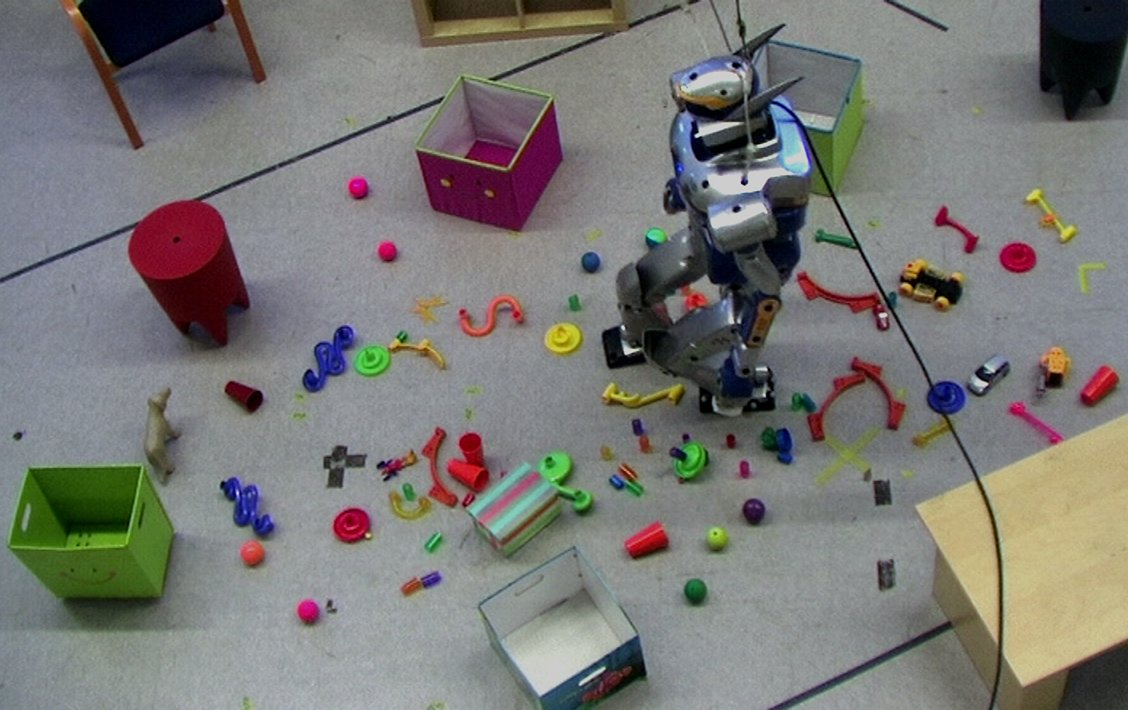
\includegraphics[width=\textwidth]{src/chap2-suivi-trajectoire/demo.jpg}
  \end{center}
  \caption{HRP-2 marchant dans un environnement extrêmement encombré
    tout en évitant des obstacles. La position finale est atteinte
    avec une précision de $\pm 3\mathrm{cm}$. L'erreur finale est la
    conséquence du bruit impactant l'estimation de la position du
    robot ainsi que de la dérive accumulée sur la fin de la
    trajectoire qu'il n'est pas possible de corriger, faute de
    temps. \label{fig:scenario}}
\end{figure}


Ensuite, le nouveau pas est validé. La décision se fonde sur le
raisonnement géométrique suivant: le pied d'HRP-2 ne peut pas entrer
en collision avec lui-même. Par conséquent, les seules collisions
possibles sont qu'un pied entre en collision avec le second. De ce
fait, si l'on ignore les configurations rares du type, ``le robot
croise les jambes en marchant'', possibles, mais aux limites des
capacités articulaires des jambes, on peut tenir le raisonnement
suivant: on peut toujours déplacer un pas du pied gauche vers la
gauche sans entrer en collision et un pas du pied droit vers la droite
sans entraîner de collision. De même on peut toujours faire tourner la
structure vers l'extérieur sans provoquer de collisions. L'heuristique
suivante est donc utilisée pour valider les pas. Elle est, évidemment,
sous-optimale, mais est sûre et a un coût en temps de calcul quasi
nul.


Si la correction est invalidée pour une des deux raisons précédemment
décrites, elle est alors abandonnée. À la prochaine phase de double
support, une nouvelle correction sera calculée et une nouvelle phase
de validation sera tentée. Dans la mesure où l'erreur de
positionnement croît lentement, il y a alors deux cas:
\begin{itemize}
\item Dans le premier, le signe de l'erreur de positionnement
  $\mathbf{\delta {x}}$ a changé, ce qui signifie que l'erreur de
  localisation était faible et qu'il n'était pas critique de la
  corriger maintenant,
\item Dans le second, le signe de l'erreur reste constant et il sera
  possible de corriger l'erreur, car la direction dans laquelle la
  correction est possible s'inverse en passant d'un pas avec le pied
  gauche à un pas avec le pied droit.
\end{itemize}

Ce système empirique a été validé avec succès sur le robot HRP-2. Un
objectif pour le futur est de remplacer cette heuristique par une
validation complète de la trajectoire de pas modifiée. Une stratégie
telle que celle décrite dans \cite{10perrin.icra} pourrait alors être
envisagée.

\section{Résultats expérimentaux}\label{exp}


La méthode proposée a été validée sur la plate-forme
HRP-2\index{HRP-2} grâce au scénario suivant: le robot doit naviguer
dans un environnement particulièrement contraint tout en enjambant des
obstacles. La longueur de la trajectoire est approximativement de
$2.5\mathrm{m}$ et est exécutée en environ $40\mathrm{s}$.


Ce scénario démontre que l'utilisation de ce schéma de contrôle permet
une navigation fiable. Le robot atteint l'objectif fixé avec une
précision de quelques centimètres tandis que le positionnement final
en utilisant un schéma de contrôle en boucle ouverte a une erreur de
plus ou moins 50 centimètres. De plus, ce schéma de contrôle est
robuste aux pertes de suivi et à des estimations peu précises par le
système de localisation. En effet, l'expérience s'appuie sur un
système de capture de mouvement pour localiser le robot. Ces derniers
sont extrêmement précis -- précision au millimètre dans les cas
favorables -- mais nécessitent un environnement dégagé ce qui n'est
pas le cas ici. Les marqueurs posés sur le pied sont parfois occlus
par les obstacles ce qui fait varier la précision durant le
mouvement. Ce comportement ne perturbe pas le schéma de correction qui
peut atteindre la position finale sans problème.


La vidéo de l'expérience est disponible sur internet:%
\vspace{-.1cm}%
\begin{center}\url{http://youtu.be/cUZ0nNiPs70}\end{center}%
La figure \ref{fig:scenario}
fournit un aperçu de l'expérience réalisée. Le robot part de la droite
et marche au travers des obstacles jusqu'à arriver à son but, sur la
partie gauche de l'image.

Dans ce contexte, la précision atteinte est de $\pm 2
\mathrm{cm}$. Cette trajectoire a été jouée cinq fois consécutivement
sans donner lieu à une collision avec un obstacle ou à une
autocollision. En utilisant un mouvement réalisant de plus petits pas,
la précision peut atteindre $1 \mathrm{cm}$. Les petits pas
nécessitent une accélération moindre du haut du corps et les effets
dynamiques mal modélisés par le modèle linéaire se font moins
ressentir, il en découle une erreur de positionnement des empreintes
de pas plus faible. L'algorithme de correction pour sa part dispose de
davantage de pas pour pouvoir réaliser des corrections. Ces deux
facteurs jouant pour améliorer la précision du suivi de trajectoire.


\section{Conclusion}\label{conclusion}


Cette section est divisée en deux et sert deux objectifs distincts. La
première partie est une introduction à la robotique humanoïde et
explique, en partant des relations fondamentales de la physique,
certains résultats récents de la littérature afin de fournir tous les
outils permettant de réaliser une tâche de locomotion pour un robot
humanoïde. Les robots humanoïdes alliant à la fois sous-actionnement
et redondance nécessitent des stratégies adaptées afin de pouvoir
générer des mouvements dans un temps raisonnable. En effet, le
problème en robotique humanoïde n'a jamais été de prévoir le mouvement
et la dynamique de corps dont les mouvements relatifs sont
contraints. Ces équations fondamentales de la physique sont connues
depuis longtemps. Le véritable enjeu est de trouver des modèles
calculatoires adaptés permettant un compromis idéal entre réalisme,
expressivité et réactivité. Différents outils de l'État de l'Art ont
été détaillés et sont assemblés pour former une plate-forme robotique
cohérente. La seconde partie propose un contrôleur pour le suivi de
trajectoire boucle fermée afin d'autoriser la navigation de précision
pour le robot humanoïde HRP-2\index{HRP-2}. Cette section montre la
barrière à franchir pour passer d'une trajectoire simulée qui semble
réalisable à une application robotique fonctionnelle où la réalité
physique et l'incertitude d'exécution inhérente à la robotique réelle
jouent un rôle prépondérant. Nous avons essayé de montrer que des
mouvements complexes nécessitent des algorithmes complexes qui seront
difficiles, même à terme, à passer dans les contrôleurs temps réels
des robots. De ce fait, si l'on veut pouvoir dépasser la simple marche
dans un sol plan, il faudra sans doute passer par des stratégies
d'adaptation locales et réactives du plan plutôt que par une
replanification globale, ce que les approches récentes tendent à
réaliser.

%\chapter{Primitives de mouvement}
\label{chap:primitive}

\epigraph{Vous n'avez qu'à marcher de vertus en vertus.}{Jean
  Racine\\\emph{Britannicus}}
\clearpage

\section{Problématique}

\lettrine[lines=2, lraise=0.1, nindent=0em, slope=-.5em]%
{L}{e} chapitre précédent a introduit la possibilité d'asservir une
trajectoire de marche sur un robot humanoïde. Cependant, les tâches
accomplies par les robots humanoïdes ne se limitent pas à la
locomotion et il est intéressant de se demander s'il est possible de
combiner aux tâches de navigation d'autres tâches asservies par les
données capteurs afin de réaliser des comportements complexes. De
manière indirecte, la question qui se pose ici est celle de la limite
à placer entre d'une part raisonnement numérique et d'autre part
raisonnement logique. Ce problème récurrent de la robotique et pour
lequel il n'existe pas, de consensus au sein de la communauté trouve
ici une solution élégante. En effet, un contrôleur fondé sur le
paradigme de la pile de tâches\index{pile de tâches} ne se limite pas
à une description d'objectifs ou de contraintes robotiques dans des
espaces plus naturels que l'espace des configurations ou l'espace
cartésien, il ouvre surtout la voie à des mécanismes de supervision
décidant à quel moment insérer telle ou telle tâche à un niveau de
priorité donné. La pile de tâches réalise donc la jonction entre d'une
part, le monde du calcul numérique puisque la finalité du système est
de calculer la commande du système et d'autre part le monde de la
logique dans lequel les utilisateurs humains souhaitent exprimer leur
\emph{desiderata} au système robotique: va jusqu'à la cuisine,
apporte-moi la bouteille, ouvre la porte, etc. Il est clair que ce
type d'ordre nécessite la résolution d'abstractions et que la logique
mathématique semble être un moyen particulièrement adapté pour y
parvenir. Ces mécanismes de décision de haut niveau sont appelés
``superviseurs'' et ont pour objectif d'instancier et d'orchestrer
tous les composants d'une architecture robotique. Dans le cadre de
notre architecture, il faut donc pouvoir instancier des piles de
tâches à partir d'une description de haut niveau des ordres passés au
robot. Ce chapitre propose un langage de description des tâches
permettant de faire le lien entre représentation logique et
représentation numérique.


Nous allons commencer par détailler l'état de l'Art et en particulier
les autres travaux ayant trait aux architectures robotiques haut
niveau et à l'ordonnancement de tâches ainsi que plus généralement aux
applications robotiques complexes. Dans un second temps, le langage de
description sera décrit et quelques scénarii types seront
démontrés. Enfin, nous nous concentrerons sur les problèmes
d'asservissement posés par les robots humanoïdes avant de conclure.


\section{État de l'Art}


La perception et l'exécution de tâches asservies en robotique
représentent deux domaines particulièrement actifs. Un livre de
référence sur la localisation robotique et le SLAM\index{Simultaneous
  Localization and Mapping (SLAM)}, le domaine lié à la cartographie
et localisation simultanée en robotique est \cite{05thrun}. Les
travaux de navigation en robotique humanoïdes sont plus rares. On peut
citer les travaux de James Kuffner, Joel Chestnutt, Koichi Nishiwaki
-- \begin{CJK*}{UTF8}{min}正西脇 光一\end{CJK*} --
  \cite{05michel.humanoids,05ozawa.smc,03chestnutt.humanoids,02nishiwaki.rsj}
  de l'Université de Freiburg en Allemagne \cite{10osswald.icra}. Dans
  le domaine la vision pour les humanoïdes, l'utilisation de
  l'asservissement visuel a été tenté \cite{10dune.iros} ainsi que des
  techniques de SLAM telles que
  \cite{06stasse.iros,09kwak.humanoids}. Une introduction à
  l'asservissement visuel\index{asservissement visuel} est
  \cite{06chaumette.ram,07chaumette.ram}. La possibilité d'utiliser un
  robot humanoïde pour la modélisation automatique d'objets 3D a
  également été envisagée par \cite{09foisotte.icra,08stasse.ras}. Une
  approche fondée sur la replanification à partir de données vision
  sur HRP-2\index{HRP-2} a également été publiée dans
  \cite{11dang.humanoids}.


\section{Description d'un mouvement robotique complexe}


Décrire le comportement d'une pile de tâches\index{pile de tâches}
revient à décrire deux éléments primordiaux: d'une part les tâches
exprimées dans le solveur et de l'autre les différents changements
d'état de la pile au cours du mouvement. Concernant les
tâches\index{tâche}, il s'agit ici de représenter des fonctions
mathématiques génériques ne présentant pas de point commun permettant
une représentation générique de ces dernières. Par exemple si l'on se
limitait aux fonctions linéaires $\mathbf{A}(t) \mathbf{x} +
\mathbf{b}(t)$, encoder la matrice $\mathbf{A}$ et le vecteur
$\mathbf{b}$ serait envisageable pour un ensemble discret de valeurs
$t$ données. Le cas évoqué est trop contraint pour notre problème et
les modélisations informatiques développées dans le
\autoref{chap:chap1} n'aident pas: elles ont pour but de venir fournir
un modèle pour l'expression d'une fonction mathématique sous la forme
d'un algorithme et non pas sous la forme d'une donnée structurée
pouvant facilement être encodée. Le choix a donc été fait de définir
un ensemble de tâches permettant de réaliser un certain nombre
d'actions intéressantes. Rien n'empêche alors cet ensemble de
``primitives'' d'être étendu au cours du temps mais il nécessite
l'extension du modèle de description défini ici.


La seconde partie est la représentation des changements d'état. Un
changement d'état du solveur survient quand une tâche est: ajoutée,
supprimée ou bien encore quand sa priorité est modifiée. De manière
générale les transitions peuvent être, soit temporelles -- avance de 5
mètres puis saisis la poignée de la porte --, soit logique -- si tu es
à moins de 10 cm de la position finale, arrête-toi --. Pour comprendre
la stratégie choisie, il faut garder à l'esprit que pour réaliser un
scénario complexe certains comportements seront intégrés dans la
boucle temps réel tandis que d'autres -- typiquement les informations
capteurs -- seront traitées à l'extérieur. Les deux catégories
d'événements, temporelle ou logique, ne mettent pas en jeu les mêmes
mécanismes. Les événements temporels sont décidés à l'avance et
doivent être exécutés avec une grande précision pour assurer un
comportement correct du système tandis que les événements logiques
sont le résultat d'un mécanisme de décision externe.

De ce fait, la stratégie adoptée a été de permettre la représentation
de transitions temporelles dans le modèle de description uniquement
tandis que l'on considère que les transitions événementielles, de fait
plus lentes et difficiles à encoder, sont gérées à l'extérieur du
contrôleur par un logiciel décisionnel ayant la possibilité de
regénérer le mouvement s'il devient invalide suite à la réception
d'une nouvelle donnée capteur. De nombreux logiciels adaptés à cette
tâche ont été développés tel que SMACH\footnote{Site web officiel:
  \url{http://www.ros.org/wiki/smach}}.


\subsection{Primitive de mouvement}
\index{primitive de mouvement}

La première tâche a été de définir des primitives de mouvement de
haut niveau. Les primitives proposées sont:
\begin{enumerate}
\item La locomotion\index{locomotion}: mouvement synchronisé des deux
  jambes et du centre de masse du robot pour réaliser un déplacement
  tout en assurant sa stabilité.
\item La manipulation\index{manipulation} et le contact: mouvement
  réalisant le placement d'une partie spécifiée du robot à un
  emplacement donné dans l'espace euclidien. La tâche peut contraindre
  la position et/ou la rotation du corps à positionner.
\item Regard ou asservissement visuel\index{asservissement visuel}: le
  robot doit maintenir un point dans son champ de vision.
\end{enumerate}


\subsection{Primitive de locomotion}

Une tâche de locomotion est définie initialement comme une série de
points de contact à réaliser pour atteindre une position
finale. Chacun des points de contact\index{point de contact} étant
annoté par l'effecteur devant réaliser le contact à cet endroit. À
partir de ces informations, une trajectoire des effecteurs réalisant
les appuis est déduite ainsi que du centre de masse pour préserver
l'équilibre dynamique du système. Afin de pouvoir utiliser les
techniques décrites dans le \autoref{chap:suivi}, nous nous limiterons
à la marche sur un sol plat utilisant le pied gauche et le pied droit
du robot. Le calcul de la trajectoire des effecteurs et du centre de
masse est encore un problème ouvert à l'heure actuelle. Les modèles
simples peuvent être embarqués dans les contrôleurs au prix de
nombreuses simplifications détaillées dans le chapitre précédent
tandis que les modèles les plus compliqués nécessitent une résolution
hors du contrôleur rendant le comportement du système non réactif. Le
chapitre précédent a proposé une stratégie pour fusionner les
avantages des deux approches. Nous considérons ici la totalité de
l'approche développée au cours du chapitre précédent comme une
implémentation d'une primitive de locomotion. En particulier, l'erreur
de positionnement du robot est considérée comme une entrée de la
primitive de mouvement.


\subsubsection{Tâche d'alignement de deux repères}

Cette primitive de mouvement repose principalement sur la définition
d'une tâche où le solveur doit positionner un corps du robot à un
endroit précis à la fois en rotation et en translation. C'est cette
tâche qui va permettre de faire suivre la trajectoire des pieds
notamment.

\begin{figure}
  \begin{center}
    \begin{equation}
      \left (
      \begin{array}{cccc}
        \cline{1-4}
        \multicolumn{1}{|c}{R_{11}} & R_{12} & R_{13} & \multicolumn{1}{|c|}{t_x} \\
        \multicolumn{1}{|c}{R_{21}} & R_{22} & R_{23} & \multicolumn{1}{|c|}{t_y} \\
        \multicolumn{1}{|c}{R_{31}} & R_{32} & R_{33} & \multicolumn{1}{|c|}{t_z} \\
        \cline{1-4}
        0 & 0 & 0 & 1
      \end{array}
      \right )
    \end{equation}
  \end{center}
  \caption{Structure d'une matrice homogène représentant un élément de
    $\text{SE}(3)$: les coefficients $R_{i,j}$, $(i,j) \in \{1,
    \dotsc, 3\}$ forment la matrice de rotation associé à la
    transformation et $\{t_x, t_y, t_z\}$ le vecteur de
    translation. Une matrice de rotation ayant elle-même une forme
    contrainte: elle doit être une matrice orthogonale de déterminant
    1. \label{fig:matrixhomo}}
\end{figure}


Soit $\mathbf{M}, \mathbf{M}^{*} \in \text{SE}(3)^2$
respectivement la position actuelle du corps du robot et la position
de référence à atteindre. On peut alors définir l'erreur de cette
tâche comme:

\begin{equation}\label{eq:featurepoint6d}
  \mathbf{e} = \mathbf{M} (\mathbf{M}^{*})^{-1}
\end{equation}

On remarquera que dans (\autoref{eq:featurepoint6d}), $\mathbf{e}$ est
un élément de $\text{SE}(3)$. Les éléments de $\text{SE}(3)$ peuvent
s'exprimer de nombreuses façons différentes: matrice homogène -- 16
paramètres --, translation et quaternion -- 7 paramètres
--\index{quaternion}, vecteur de rotation -- 6 paramètres --
\index{vecteur (de rotation)}, etc. Il faut garder à l'esprit qu'une
paramétrisation minimale de $\text{SE}(3)$ nécessite six
paramètres. De fait, tout représentation utilisant un espace de
dimension supérieure vient avec un ensemble de contraintes à respecter
car tous les éléments de cet espace de dimension supérieur ne peuvent
faire partie de $\text{SE}(3)$. Par exemple, une matrice homogène a une
structure bien particulière tel qu'illustré sur la
\autoref{fig:matrixhomo}.

De fait, les représentations non minimales ne constituent pas une
solution acceptable pour représenter notre erreur, car elles
provoquent l'insertion de contraintes supplémentaires inutiles dans le
problème d'optimisation. Il faut donc choisir pour représenter
$\mathbf{e}$ une représentation minimale, dans notre cas par une
translation et une rotation autour d'un axe.

En effet, toute rotation peut être représentée par trois paramètres
\mbox{$\mathbf{\theta} = (\alpha, \beta, \gamma) \in \mathbb{R}^3$}. Le
vecteur $(\alpha, \beta, \gamma)$ normalisé représentant l'axe autour
duquel la rotation s'effectue et la norme du vecteur
$|\mathbf{\theta}|$ la quantité de rotation réalisée autour de cet
axe, voir \autoref{fig:utheta}.

\begin{figure}
  \begin{center}
    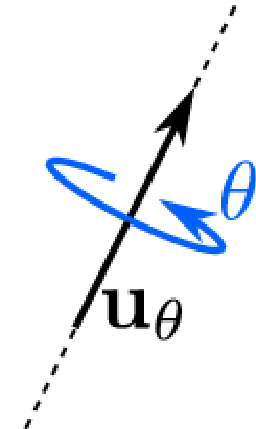
\includegraphics[width=.1\linewidth]{src/chap3-primitive-mouvement/utheta.pdf}
  \end{center}
  \caption{Représentation d'une rotation par un axe de rotation $u$ et
    une quantité de rotation $\theta$. Une représentation minimale à
    trois paramètres est possible en posant: $\theta = |u|$. \label{fig:utheta}}
\end{figure}


Cette représentation est minimale, car la translation est représentée
par trois paramètres et la rotation par trois paramètres:

\begin{equation}
  \mathbf{e} = \left(
  \begin{array}{c}
    t_x\\
    t_y\\
    t_z\\
    \theta_x\\
    \theta_y\\
    \theta_z
  \end{array}
  \right)
\end{equation}

En considérant les trois premiers éléments du vecteur d'erreur ou bien
les trois derniers, on peut restreindre la tâche à positionner le corps
respectivement en translation ou en rotation uniquement.


\subsubsection{Tâche de position du centre de masse}


Le second type de tâche nécessaire pour définir la primitive de
locomotion est la tâche de positionnement du centre de masse.

Cette tâche nécessite la connaissance du poids de tous les corps du
robot $m_i$ où $i \in \mathcal{B}$. $\mathcal{B}$ l'ensemble des corps
du robot. Le centre de masse\index{centre de masse} du robot est alors
défini comme le barycentre des centres de masse de chaque corps:

\begin{equation}
  \mathbf{x} = \frac{1}{\sum_{i \in \mathcal{B}} m_i} \sum_{i \in \mathcal{B}} m_i \mathbf{x}_i
\end{equation}

$\mathbf{x}$ représentation la position du centre de masse du robot et
$\mathbf{x}_i$ la position du centre de masse du corps $i$.

L'erreur de positionnement du centre de masse est alors simplement:

\begin{equation}
  \mathbf{e} = \mathbf{x} - \mathbf{x}^{*}
\end{equation}

La définition de l'erreur ne posant pas de difficulté ici car
$\mathbf{x}$ est un élément de $\mathbb{R}^3$.


\subsubsection{Définition de la primitive de locomotion}

Une tâche de locomotion est par nature critique: un mauvais suivi de
la trajectoire de référence du centre de masse ou bien encore de la
trajectoire des pieds aboutit à une perte de l'équilibre du robot. De
ce fait, établir une priorité entre ces tâches n'a pas de sens. On
préférera donc exprimer ces trois tâches -- pied gauche, pied droit et
centre de masse -- de la façon suivante:

\begin{equation}
  \mathbf{e} = \left(
  \begin{array}{c}
    \mathbf{e}_{\text{pied gauche}}\\
    \mathbf{e}_{\text{pied droit}}\\
    \mathbf{e}_{\text{centre de masse}}
  \end{array}\right)
\end{equation}

Les équations formulées dans cette section peuvent enfin être
paramétrées par le temps courant $t$ afin de permettre une
modification de la valeur de référence notée $\mathbf{M}^*$ ou
$\mathbf{x}^*$ selon les cas et permettre le suivi d'une trajectoire
plutôt que l'atteinte d'une référence constante.


Comme décrit dans le chapitre précédent, l'erreur des tâches décroît
exponentiellement -- dans le cas où la référence reste constante
--. Un suivi suffisamment précis de la trajectoire est alors
réalisable en augmentant suffisamment $\lambda$ le gain associé à la
tâche. Dans la mesure où l'erreur initiale de cette tâche est nulle --
le mouvement commence à la position actuelle du robot -- et varie de
manière continue, la tâche ne génère pas de grandes vitesses
articulaires malgré le gain important.


\subsubsection{Primitive de manipulation}


La primitive de manipulation est une instance directe de la tâche
d'alignement de repères présentée dans la section précédente. Elle
est utilisée pour placer la main à un endroit donné afin de saisir un
objet. Le déplacement d'un bras du robot ne mettant pas en jeu
l'équilibre du robot tant qu'elle se déplace peu rapidement et sans
perturber la tâche de suivi du centre de masse, on peut simplement
corriger l'erreur de positionnement de la main avec une interpolation
linéaire pour amener la main à la position désirée.


\subsubsection{Primitive de regard}


La dernière primitive introduite ici concerne l'asservissement de la
trajectoire du robot afin de préserver des amers dans une zone où
elles sont détectables par les capteurs du robot. Sur le robot HRP-2,
seules des caméras sont à la disposition des utilisateurs et leur
placement dans la tête permet naturellement de définir une tâche de
``regard'' où l'utilisateur souhaite garder un point au centre de
l'image captée par une caméra du robot.

Soit \mbox{$M = (X, Y, Z) \in \mathbb{R}^3$} un point 3D dont les
coordonnées sont définies par rapport à la position de la caméra du
robot et \mbox{$m = (x, y) \in \mathbb{R}^2$} sa projection sur le
plan image de la caméra\index{géométrie projective}. On a alors la
relation suivante:

\begin{equation}
  \mathbf{m} = \left(
  \begin{array}{c}
    x\\
    y
  \end{array}
  \right) = \left(
  \begin{array}{c}
    X / Z\\
    Y / Z
  \end{array}
  \right)
\end{equation}


Une fois de plus l'erreur se définit par la soustraction usuelle:

\begin{equation}
  \mathbf{e} = \mathbf{m} - \mathbf{m}^*
\end{equation}

\begin{figure}
  \begin{center}
    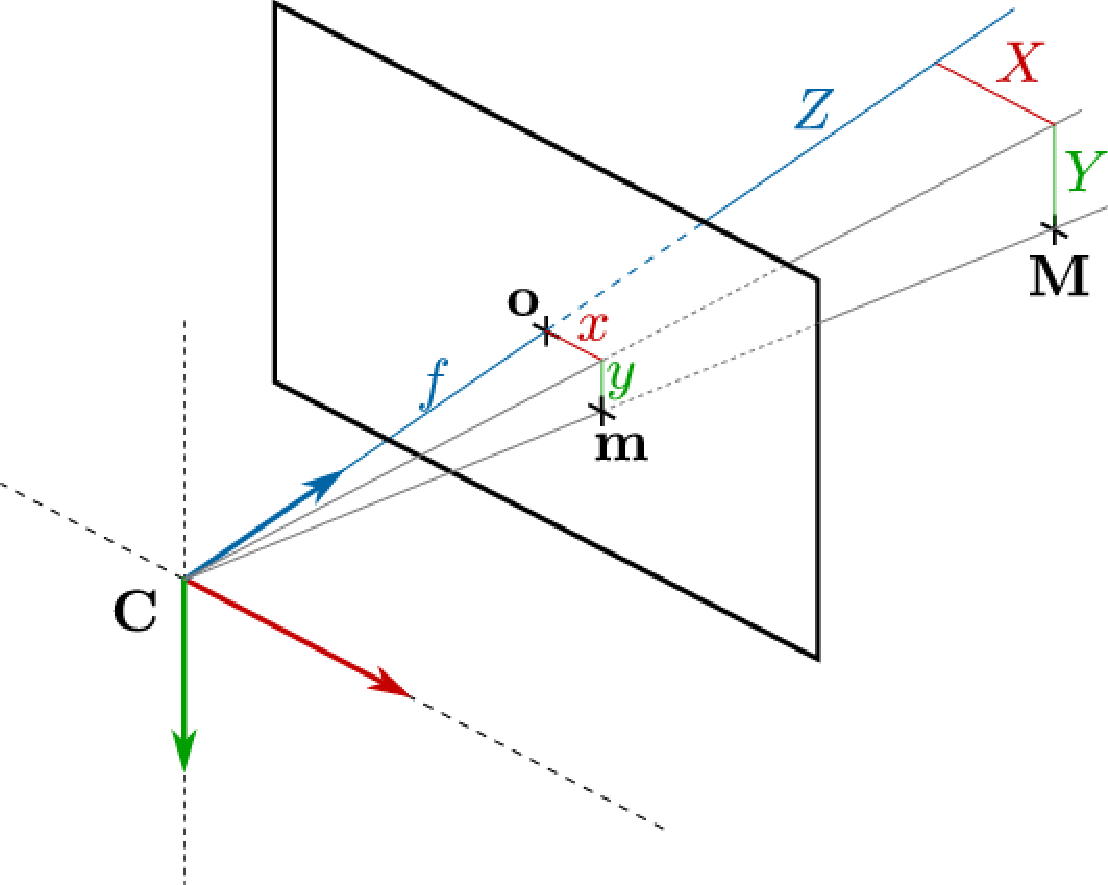
\includegraphics[width=.95\linewidth]{src/chap3-primitive-mouvement/cameraProj.pdf}
  \end{center}
  \caption{Projection du point 3D $M = (X, Y, Z)$ sur le plan image
    d'une caméra idéale. Les coordonées du point projeté sont ici $m =
    (x, y)$. $f$ est la distance focale de la caméra et $C$ le centre
    optique, deux paramètres intrinsèques de la caméra.}
\end{figure}




\subsection{Langage de description}

Le langage de description adopté est le YAML -- Yet Another Markup
Language -- \citep{yaml}\index{Yet Another Markup Language (YAML)}. Le
fichier est divisé en trois parties:
\begin{description}
\item[En-tête] fournissant les méta-informations sur le mouvement,
  notamment sa durée en secondes.
\item[Primitives de mouvement] définissant quelles primitives sont
  jouées et sur quel intervalle, ainsi que la configuration de chaque
  primitive.
\item[Primitives d'asservissement] définissant comment l'erreur de
  positionnement du robot est estimée au fil du temps.
\end{description}


\subsubsection{Primitive de locomotion}
\index{primitive!de locomotion}

Une primitive de locomotion est définie par un ensemble de points de
contacts définis sur la forme d'une pile de pas.

\begin{description}
\item[Intervalle.] Date de début et de fin de la primitive de mouvement.
\item[Empreinte de pas.] Liste des pas à effectuer. Les pas sont
  considérés comme des éléments de $\text{SE}(2)$ dans la mesure où
  l'algorithme de génération de pas fait l'hypothèse d'un sol plan.
\end{description}

Lors du chargement du plan, la génération des trajectoires de pieds et
de centre de masse initiales est réalisée hors ligne de manière
asynchrone. Tant que le calcul n'est pas terminé, il n'est pas
possible de lancer le mouvement.


\subsubsection{Primitive de manipulation}
\index{primitive!de manipulation}

Une primitive de manipulation est définie par un corps et une position
6d de référence. L'objectif est de faire coïncider le corps avec la
position 6d de référence. Cette tâche peut ne considérer que la
rotation ou la translation.

\begin{description}
\item[Intervalle.] Date de début et de fin de la primitive de manipulation.
\item[Corps à considérer.] Nom du corps à considérer. Des noms
  génériques ont été définis tels que: cheville gauche, cheville
  droite, poignet gauche, poignet droit, tête, torse et bassin.
\item[Consigne.] La position de référence vers laquelle le corps doit
  être amené. Il peut être de trois types. Soit statique, le corps
  doit maintenir sa position initiale, soit fixe dans ce cas le corps
  doit atteindre un point prédéterminé de l'espace, soit dynamique
  dans ce cas le corps doit suivre un point mobile.
\end{description}


\subsubsection{Primitive de regard}
\index{primitive!de regard}

La primitive de regard définit comment le robot peut maintenir son
regard vers un point 3D, éventuellement mobile.

\begin{description}
\item[Intervalle.] Date de début et de fin de la primitive de manipulation.
\item[Caméra à considérer.] Nom de la caméra utilisée. En pratique, la
  caméra est définie comme un corps ``virtuel'' du robot et l'on peut
  donc potentiellement aligner n'importe quelle partie du corps du
  robot vers un point donné.
\item[Consigne.] La position de référence vers lequel le corps doit
  pointer. Il peut être de deux types. Soit fixe, dans ce cas le corps
  doit pointer vers un point prédéterminé de l'espace, soit dynamique
  et dans ce cas le corps doit pointer vers un point mobile.
\end{description}


\subsubsection{Asservissement des primitives sur les données capteur}


Une fois la séquence de mouvement définie, il faut encore pouvoir
fermer la boucle sur les données capteur. Dans le cadre d'un mouvement
complexe, une stratégie intéressante est de pouvoir s'asservir
successivement sur plusieurs amers afin de planifier \emph{a priori}
quelle est la ou les amers les plus pertinentes à différents instants.


Soit $\mathcal{L}$ un système de localisation. Un système de
localisation est défini comme une fonction qui à tout instant fournit
une pose estimée d'un corps de référence du robot, dans notre cas le
bassin. On a donc:

\begin{equation}
  \begin{array}{ccc}
    \mathcal{L} : & \mathbb{R} \rightarrow & \text{SE}(2)\\
      & t \mapsto & \mathcal{L}(t)
  \end{array}
\end{equation}

Au cours du mouvement, $n$ systèmes de localisation fournissent une
estimation de la pose du robot. Une fois de plus, cette pose est
théoriquement dans l'espace 3D $\text{SE}(3)$, mais les contraintes
physiques font que seuls trois degrés de liberté doivent être
réellement estimés: $(x, y, \theta) \in \text{SE}(2)$. Ces trois
degrés correspondent à la position 2D de la projection du bassin sur
le sol. De ce fait, l'interpolation de $n$ poses 2D et la moyenne des
poses à la normalisation de l'angle $\theta$ prêt.


On associe à chaque système de localisation une fonction de poids
déterminant l'influence relative des systèmes de localisation dans
l'estimation finale de la pose:

\begin{equation}
  \begin{array}{ccc}
    m_i : & \mathbb{R} \rightarrow & \mathbb{R}\\
      & t \mapsto & m_i(t)
  \end{array}
\end{equation}

La fusion des données pour l'estimation de la pose est donc le
barycentre des poses 2d:

\begin{equation}
  \mathbf{\hat{x}}(t) = \frac{1}{\sum_{i \in n} m_i} \sum_{i \in n} m_i \mathcal{L}_i(t)
\end{equation}

En pratique, chaque système de localisation est représenté de la façon suivante:
\begin{description}
\item[Poids.] en fonction du temps. Il peut, soit être constant, soit
  varier dynamiquement.
\item[Erreur.] de positionnement en fonction du temps. Elle est fournie
  par un système de localisation externe.
\end{description}


\section{Scénarii de mouvements}


Nous allons voir ici plusieurs exemples de mouvements décrits en
utilisant le langage de description introduit dans la section
précédente. L'objectif est à la fois de démontrer la généricité de
l'approche par plusieurs scénarii différents ainsi que sa mise en
\oe uvre pratique.


\subsection{Locomotion simple}

Le premier scénario consiste en le déplacement du robot le long d'une
pile de pas prédéterminée pendant 20 secondes. La description
complète du plan est fournie par la \autoref{fig:plan_locomotion_simple}.

\begin{figure}
  \begin{center}
\begin{verbatim}
duration: 20 # durée complète du mouvement (secondes)

# Éléments de mouvement
motion:
  # Primitive de locomotion
  - walk:
      interval: [0, 20] # Date de début et de fin de la primitive

      # Pile de pas
      footsteps:
      - {x: 0.15, y: -0.19, theta: 0.}
      - {x: 0.15, y: +0.19, theta: 0.1}
      # etc.
\end{verbatim}
  \end{center}
  \caption{Plan de mouvement pour une séquence de marche non asservie.\label{fig:plan_locomotion_simple}}
\end{figure}

La marche est effectuée en boucle ouverte et l'erreur d'exécution
n'est pas compensée. Chaque pas est exprimé relativement au pas
précédent. Le corps effectuant chaque contact peut être déduit de la
séquence d'empreinte de pas: si la translation en $y$ du premier pas
dispose d'un signe négatif, le premier pas est effectué avec le pied
droit, sinon avec le pied gauche. L'alternance pied gauche/pied droit
à chaque pas est ensuite implicite.


Il n'y a pas, à ce niveau de vérification de la faisabilité des
pas. C'est le rôle du planificateur de s'assurer préalablement à la
génération du plan de mouvement que la séquence est réalisable.

\begin{figure}
  \begin{center}
    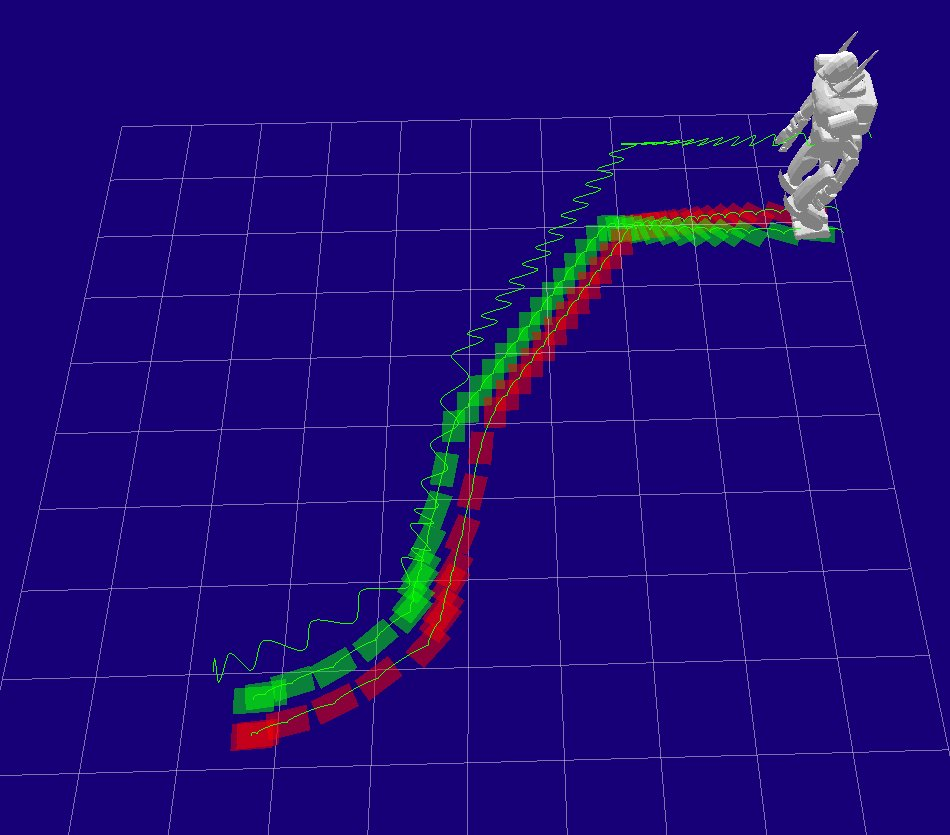
\includegraphics[width=.95\linewidth]{src/chap3-primitive-mouvement/footsteps1.jpg}
  \end{center}
  \caption{Exemple de pile de pas à partir de laquelle une primitive
    de locomotion peut être calculée.}
\end{figure}


\FloatBarrier

\subsection{Locomotion asservie}

On peut se demander désormais comment asservir la locomotion en
utilisant un composant de localisation. La
\autoref{fig:plan_locomotion_asservie} fournit une version alternative
du plan précédent ajoutant la correction de pas introduite dans le
\autoref{chap:suivi}.

\begin{figure}
  \begin{center}
\begin{verbatim}
duration: 20 # durée complète du mouvement (secondes)

# correction maximum autorisée sur un pas (x, y en mètre, theta en radians)
maximum-correction-per-step: {x: 0.02, y: 0.02, theta: 0.05}

# Éléments de mouvement
motion:
  # Primitive de locomotion
  - walk:
      interval: [0, 20] # Date de début et de fin de la primitive

      # Pile de pas
      footsteps:
      - {x: 0.15, y: -0.19, theta: 0.}
      - {x: 0.15, y: +0.19, theta: 0.1}
      # etc.

# Asservissement des tâches
servoing:
  # Asservissement via le système de capture de mouvements.
  - mocap:
      weight: 1.
      tracked-body: left-ankle
      perceived-body: left-foot
\end{verbatim}
  \end{center}
  \caption{Plan de mouvement pour une séquence de marche asservie sur
    un système de localisation -- ici un système de capture de
    mouvement --.\label{fig:plan_locomotion_asservie}}
\end{figure}

La seconde partie du plan décrit que l'erreur de positionnement
provient d'un unique système de localisation. Dans ce cas, un système
de capture de mouvement. Plusieurs systèmes de localisation ont été
testés pour fournir une estimation de la position du robot au cours du
mouvement:

\begin{description}
\item[Capture de mouvement.] Ce système permet une localisation
  quasi-parfaite permettant de s'abstraire de la plupart des problèmes
  de perception.
\item[Suivi d'un objet.] Un système réalisant le suivi d'un objet dans
  l'image captée par une caméra du robot et reconstituant sa
  position 3D peut également être utilisé. Dans ce cas, on suppose
  l'objet fixe dans le monde et on en déduit la position du robot.
\item[SLAM.] Les techniques de SLAM -- Simultaneous Localization and
  Mapping -- permettent de cartographier l'environnement tout en
  fournissant une estimation de la position actuelle du robot. La
  carte enregistrée permet d'assurer une localisation sans dérive
  quelque soit la longueur du mouvement à condition de pouvoir
  identifier des amers précédemment détectées régulièrement le long
  du mouvement.
\end{description}

\begin{figure}
  \begin{center}
\begin{verbatim}
duration: 20 # durée complète du mouvement (secondes)

# correction maximum autorisée sur un pas (x, y en mètre, theta en radians)
maximum-correction-per-step: {x: 0.02, y: 0.02, theta: 0.05}

environment:
  - object:
      name: table
      planned:
        position:
          x: 1.75
          y: 0.3
          z: -0.3
          rx: 0.
          ry: 0.
          rz: 2.

# Éléments de mouvement
motion:
  # Primitive de locomotion
  - walk:
      interval: [0, 20] # Date de début et de fin de la primitive

      # Pile de pas
      footsteps:
      - {x: 0.15, y: -0.19, theta: 0.}
      - {x: 0.15, y: +0.19, theta: 0.1}
      # etc.

# Asservissement des tâches
servoing:
  # Asservissement via le système de capture de mouvements.
  - visp:
      interval: [0, 20] # Date de début et de fin de l'élément d'asservissement.
      weight: 1.
      object-name: table
      position: /tracker_mbt/resultTransform
      camera-velocity: /tracker_mbt/camera_velocity
      frame-name: cameraBottomLeft
\end{verbatim}
  \end{center}
  \caption{Plan de mouvement pour une séquence de marche asservie sur
    un système de suivi d'objet.}
\end{figure}

\begin{figure}
  \begin{center}
\begin{verbatim}
duration: 20 # durée complète du mouvement (secondes)

# correction maximum autorisée sur un pas (x, y en mètre, theta en radians)
maximum-correction-per-step: {x: 0.02, y: 0.02, theta: 0.05}

# Éléments de mouvement
motion:
  # Primitive de locomotion
  - walk:
      interval: [0, 20] # Date de début et de fin de la primitive

      # Pile de pas
      footsteps:
      - {x: 0.15, y: -0.19, theta: 0.}
      - {x: 0.15, y: +0.19, theta: 0.1}
      # etc.

# Asservissement des tâches
servoing:
  # Asservissement via le système de localisation externe (SLAM).
  - control-ros:
      weight: 1.
      topic: /error
      signal: error
\end{verbatim}
  \end{center}
  \caption{Plan de mouvement pour une séquence de marche asservie sur
    un algorithme de SLAM. En pratique, dans ce cas l'évaluation de
    l'erreur est totalement effectuée hors du contrôle.}
\end{figure}

\FloatBarrier

\subsection{Scénario d'atteinte avec équilibre quasi statique}

Dans ce scénario, le robot place son poignet a un point prédéterminé
tout en préservant la position de son centre de masse. Le plan de
mouvement est détaillé dans la \autoref{fig:plan_atteinte}.

\begin{figure}
  \footnotesize
  \begin{center}
\begin{verbatim}
duration: 10 # durée complète du mouvement (secondes)

motion:
# Fixe la position des pieds.
  - task:
      # Date de début et de fin de la primitive.
      interval: [0, 10]
      # Type de la tâche: positionnement d'un corps.
      type: feature-point-6d
      # Corps à positionner (cheville gauche).
      operational-point: left-ankle
      # Gain de la tâche.
      gain: 1.
      # Consigne de la tâche: aucun mouvement.
      reference: static
      # Contrainte en translation *et* rotation.
      translation: on
      rotation: on
  - task:
      # Date de début et de fin de la primitive.
      interval: [0, 10]
      # Type de la tâche: positionnement d'un corps.
      type: feature-point-6d
      # Corps à positionner (cheville droite).
      operational-point: right-ankle
      # Gain de la tâche.
      gain: 1.
      # Consigne de la tâche: aucun mouvement.
      reference: static
      # Contrainte en translation *et* rotation.
      translation: on
      rotation: on
# Fixe la position du centre de masse.
  - task:
      # Date de début et de fin de la primitive.
      interval: [0, 10]
      # Type de la tâche: positionnement du centre de masse.
      type: feature-com
      # Gain de la tâche.
      gain: 1.
      # Consigne de la tâche: aucun mouvement.
      reference: static
      # Degré de liberté supplémentaires déverrouillés.
      extra-unlocked-dofs: [18., 19.] # HRP-2 chest dofs.

# Tâche d'atteinte.
  - task:
      # Date de début et de fin de la primitive.
      interval: [0, 10]
      # Type de la tâche: positionnement d'un corps.
      type: feature-point-6d
      # Corps à positionner (poignet droit).
      operational-point: right-wrist
      # Gain de la tâche.
      gain: 7.5
      # Consigne: position finale du poignet droit.
      reference: {x: 0.4, y: -0.3, z: 1.1}
      # Contrainte en translation uniquement.
      translation: on
      rotation: off
\end{verbatim}
  \end{center}
  \caption{Plan de mouvement pour une tâche d'atteinte.\label{fig:plan_atteinte}}
\end{figure}

Contrairement à la tâche de locomotion qui est totalement encapsulée
dans une primitive peu paramétrable, le scénario d'atteinte nécessite
la définition manuelle des tâches. Quatre tâches sont définies ici:
deux pour maintenir les pieds à leur place, une pour maintenir le
centre de masse à sa position initiale et une dernière qui génère le
mouvement du poignet droit.

Les tâches associées aux pieds et au centre de masse possèdent un gain
faible, car l'erreur a une erreur nulle initialement. Inversement, la
tâche associée au poignet droit a une erreur maximum initialement et
donc une vitesse maximum. Le gain permet alors de contrôler la vitesse
de réalisation de la tâche et donc, de manière indirecte, la vitesse
de déplacement du bras.

\FloatBarrier

\subsection{Scénario d'asservissement visuel de la tête}

La dernière primitive de mouvement considérée ici permet d'asservir le
regard du robot sur la position d'un point 3D, soit fixe, soit mobile
et estimé par un système externe. Le plan correspondant est la
\autoref{fig:plan_asservissement_complet}.

\begin{figure}
  \footnotesize
  \begin{center}
\begin{verbatim}
duration: 25 # durée complète du mouvement (secondes)
# correction maximum tous les deux pas
maximum-correction-per-step: {x: 0.04, y: 0.04, theta: 0.1}

environment:
  - object:
      name: table
      planned:
        position:
          x: 1.75
          y: 0.3
          z: -0.3
          rx: 0.
          ry: 0.
          rz: 2.

motion:
  # Primitive de locomotion
  - walk:
      interval: [0, 20] # Date de début et de fin de la primitive

      # Pile de pas
      footsteps:
      - {x: 0.15, y: -0.19, theta: 0.}
      - {x: 0.15, y: +0.19, theta: 0.1}
      # etc.

  # Asservissement de la tête
  - visual-point:
      interval: [0, 25]
      gain: 1.
      object-name: table
      frame-name: cameraBottomLeft

servoing:
  - visp:
      weight: 1.
      object-name: table
      position: /tracker_mbt/resultTransform
      frame-name: cameraBottomLeft
\end{verbatim}
  \end{center}
  \caption{Plan de mouvement pour une tâche de marche avec
    asservissement de la tête.\label{fig:plan_asservissement_complet}}
\end{figure}

\FloatBarrier

\section{De la difficulté à localiser un robot humanoïde}
\label{sec:chap3_localisation}


Plusieurs séries d'expérimentation ont été réalisées sur le robot
HRP-2 afin de tester le comportement des algorithmes de localisation
utilisant des capteurs embarqués.


\begin{figure}
  \begin{center}
    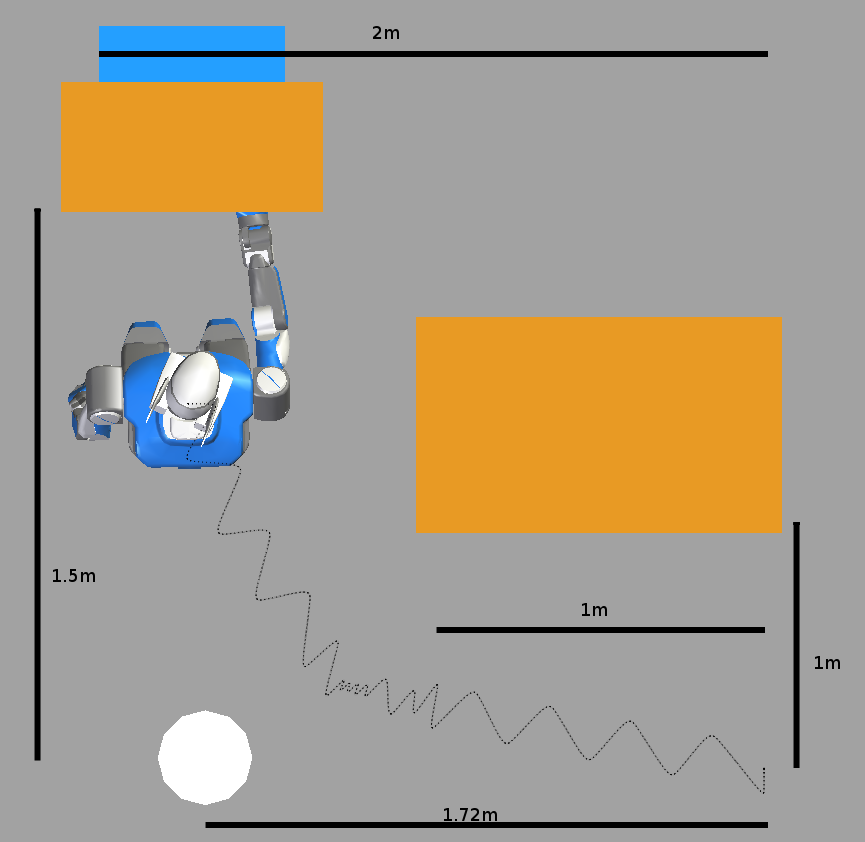
\includegraphics[width=.75\linewidth]{src/chap3-primitive-mouvement/dimensions.png}
    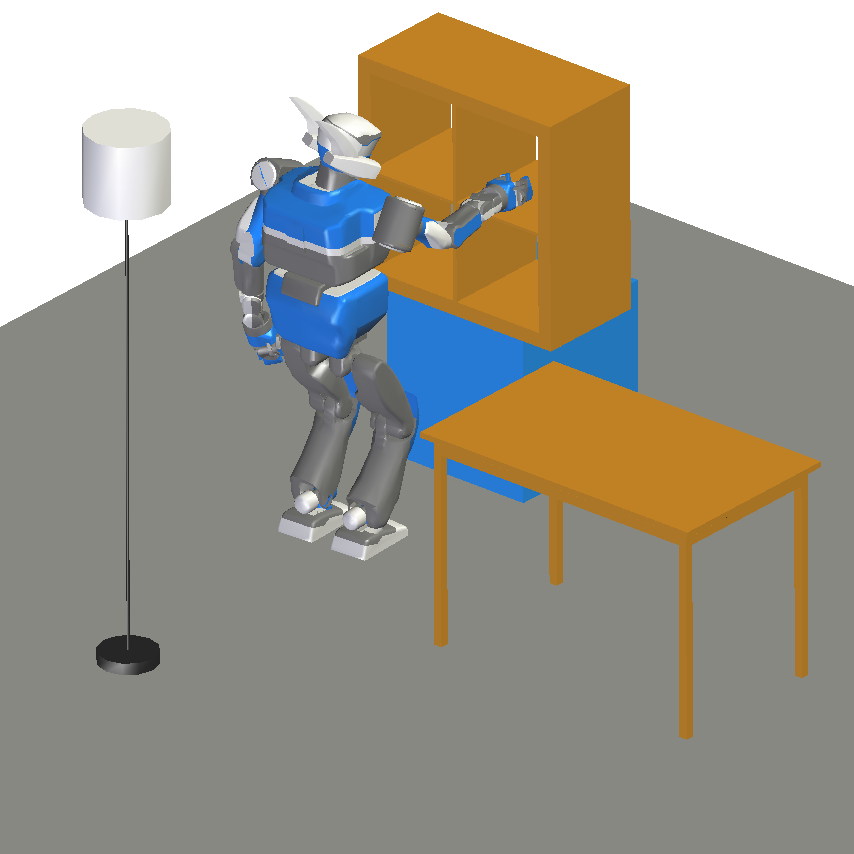
\includegraphics[width=.75\linewidth]{src/chap3-primitive-mouvement/trajectory-8.png}
  \end{center}
  \caption{Description de l'expérimentation: le robot part de la
    droite de l'image et progresse vers l'étagère située à gauche pour
    y déposer une balle. \label{fig:scenario_visu}}
\end{figure}



Le scénario proposé est le suivant: HRP-2\index{HRP-2} contourne un
obstacle, passe entre deux objets, et va poser une balle sur une
étagère. La longueur de la trajectoire de marche -- 2 mètres environ
-- et le nombre de pas génèrant une dérive suffisante pour qu'une
exécution de ce scénario échoue en boucle ouverte. En effet, passer
son bras dans une étagère est un mouvement contraint particulièrement
sensible à la position d'arrivée du robot. Une petite erreur dans le
positionnement du robot à la fin de la trajectoire engendrera une
grande erreur dans la position finale du
poignet. La \autoref{fig:scenario_visu} illustre le scénario.
L'objectif ici est d'utiliser les caméras embarquées pour construire
une carte de l'environnement puis pour localiser le robot. La
stratégie adoptée ici n'est pas du SLAM -- Simultaneous Localization
and Mapping --\index{Simultaneous Localization and Mapping (SLAM)}
dans la mesure où les images permettant de construire la carte sont
traitées hors ligne. On réalise donc un premier mouvement sans
correction afin d'acquérir une séquence d'images permettant de
construire la carte puis on utilise cette carte pour localiser le
robot durant les expérimentations suivantes. La qualité du résultat
est ensuite validée en utilisant un système de capture de mouvement.


Durant les expériences, le module de localisation a fourni une
estimation de la position du robot à 16\hertz. Les images ont une
résolution de 320x240 pixels. L'ordinateur sur lequel fonctionne le
composant de localisation est un
\mbox{Intel\textregistered~Core\texttrademark 2 CPU T7200 @ 2.00GHz}
avec 2 Gb.\ de RAM.


\subsection{Analyse de la précision du système de localisation}

La précision finale du système est illustrée par la
\autoref{fig:scenario_visu_precision}. On peut y observer une erreur à
la fin de la trajectoire d'environ 0.2 mètres en
translation. Plusieurs raisons peuvent expliquer ces mauvais
résultats:
\begin{enumerate}
\item Carte non métrique et absence de fermeture de boucle,
\item Passage dans des zones où la carte est peu dense ou dans des
  zones ne possédant que peu d'information visuelle,
\item Flexibilité du robot et/ou mauvaise identification de certains paramètres,
\end{enumerate}


Le premier point pouvant amener à une mauvaise estimation de la
localisation du robot est l'absence de fermeture de boucle. Les
techniques de localisation utilisant les informations visuelles
peuvent être divisées en deux catégories: odométrie
visuelle\index{odométrie visuelle} et localisation
``globale''. L'odométrie visuelle observe les changements entre deux
images aux temps $t_{n-1}$ et $t_n$ afin d'estimer la vitesse de la
caméra entre les deux images. Cette vitesse est ensuité intégrée pour
calculer le mouvement de la caméra. Par conséquent, il se produit une
dérive temporelle qui empêche toute tentative de localisation sur le
long terme en utilisant cette technique. Inversement, les algorithmes
utilisant une carte peuvent identifier les amers déjà détectés
auparavant et stabiliser le système. Une limite de ce mouvement est
qu'il n'est pas facile pour le système de reconnaître des amers déjà
identifiés. Il s'en suit une dérive dans l'estimation de la position
du robot.


Le second problème concerne l'environnement en lui-même: à la fin du
mouvement, le robot se trouve face au meuble ce qui rend les images
captées par les caméras vides de tout amer permettant d'effectuer
correctement la localisation. Ce problème ne peut expliquer que
partiellement la mauvaise estimation dans la mesure où l'occlusion des
caméras n'intervient qu'à l'extrême fin du mouvement.


Le dernier point pouvant amener à une mauvaise estimation de l'erreur
est lié à la mauvaise modélisation de la chaîne cinématique du
robot. Une première erreur est liée à la présence, au niveau des
chevilles du robot, d'une flexibilité passive pouvant être modélisé
sous la forme de trois ressorts: deux autorisant un mouvement en
rotation et un troisième un déplacement en translation, c'est à dire
autorisant une compression de la cheville lors de la marche. Ce
dispositif a été conçu pour absorber les chocs et protéger le capteur
de force situé dans la cheville mais insère trois degrés de liberté
non modélisés et surtout non mesurables, car dépourvu
d'encodeur. Cette déformation au niveau de la cheville est donc
ignorée dans les calculs ce qui amène à un biais sur la position
relative du pied et de la tête du robot. Ce biais est d'autant plus
critique dans ce cas que c'est la position des points de contact que
l'on essaie de corriger. Une seconde source d'erreur est la
calibration de la position de la caméra dans le robot. Les
imprécisions de la conception du robot, du système de fixation des
caméras rendent nécessaire le calcul de la position relative de la
caméra par rapport au corps auquel il est fixé, dans notre cas la
tête. Un procédé de calibration des paramètres
extrinsèques\index{paramètres extrinsèques (d'une caméra)} a donc été
mis en place pour estimer ces paramètres. Ces derniers ont été validés
en reprojetant le modèle du robot dans l'image comme illustré par la
\autoref{fig:reprojection_modele_vision}.


\subsection{Résultats de la localisation utilisant la vision sur le robot humanoïde HRP-2}

L'ensemble de ces facteurs rend la réalisation d'un algorithme de
localisation embarqué sur HRP-2\index{HRP-2} délicat. Pour réaliser
une tâche de manipulation, une précision de l'ordre du centimètre est
souvent nécessaire. Or, les mauvaises performances du système de
localisation engendrent un bruit dans le positionnement du robot qui
peut rendre l'exécution de tâches précises délicates. Dans le scénario
choisi, la tâche peut être réalisée avec succès pour certains essais,
mais le taux d'échec restant très fort, cette méthode ne peut pas
constituer une boîte noire permettant de manière automatique de
réaliser un mouvement asservi. Une façon de résoudre le problème
serait de corriger la position du bras. En effet, entre la caméra et
le bras, la chaîne cinématique est bien identifiée. On voit donc ici
que l'approche consistant à avoir plusieurs systèmes de localisation
simultanément se justifie en pratique. Un composant de localisation
``global'' tel que celui utilisé ici permet de rendre la navigation
robuste sans toutefois être suffisant pour les tâches de
manipulation. Pour ces dernières, d'autres stratégies doivent être
envisagées comme la détection dans l'image de l'objet à attraper pour
asservir la position de la pince. On voit ici que plus qu'une
localisation parfaite sur le long terme, il est plus critique pour nos
scénarii d'avoir des algorithmes de localisation locaux assurant une
erreur minimale à la fin de la réalisation de la tâche. Les
algorithmes réalisant une localisation sur le long terme étant plutôt
destinés à alimenter les algorithmes de planification que les
algorithmes de contrôle nécessitant une haute précision sur la pose
estimée du robot.




\begin{figure}
  \begin{center}
    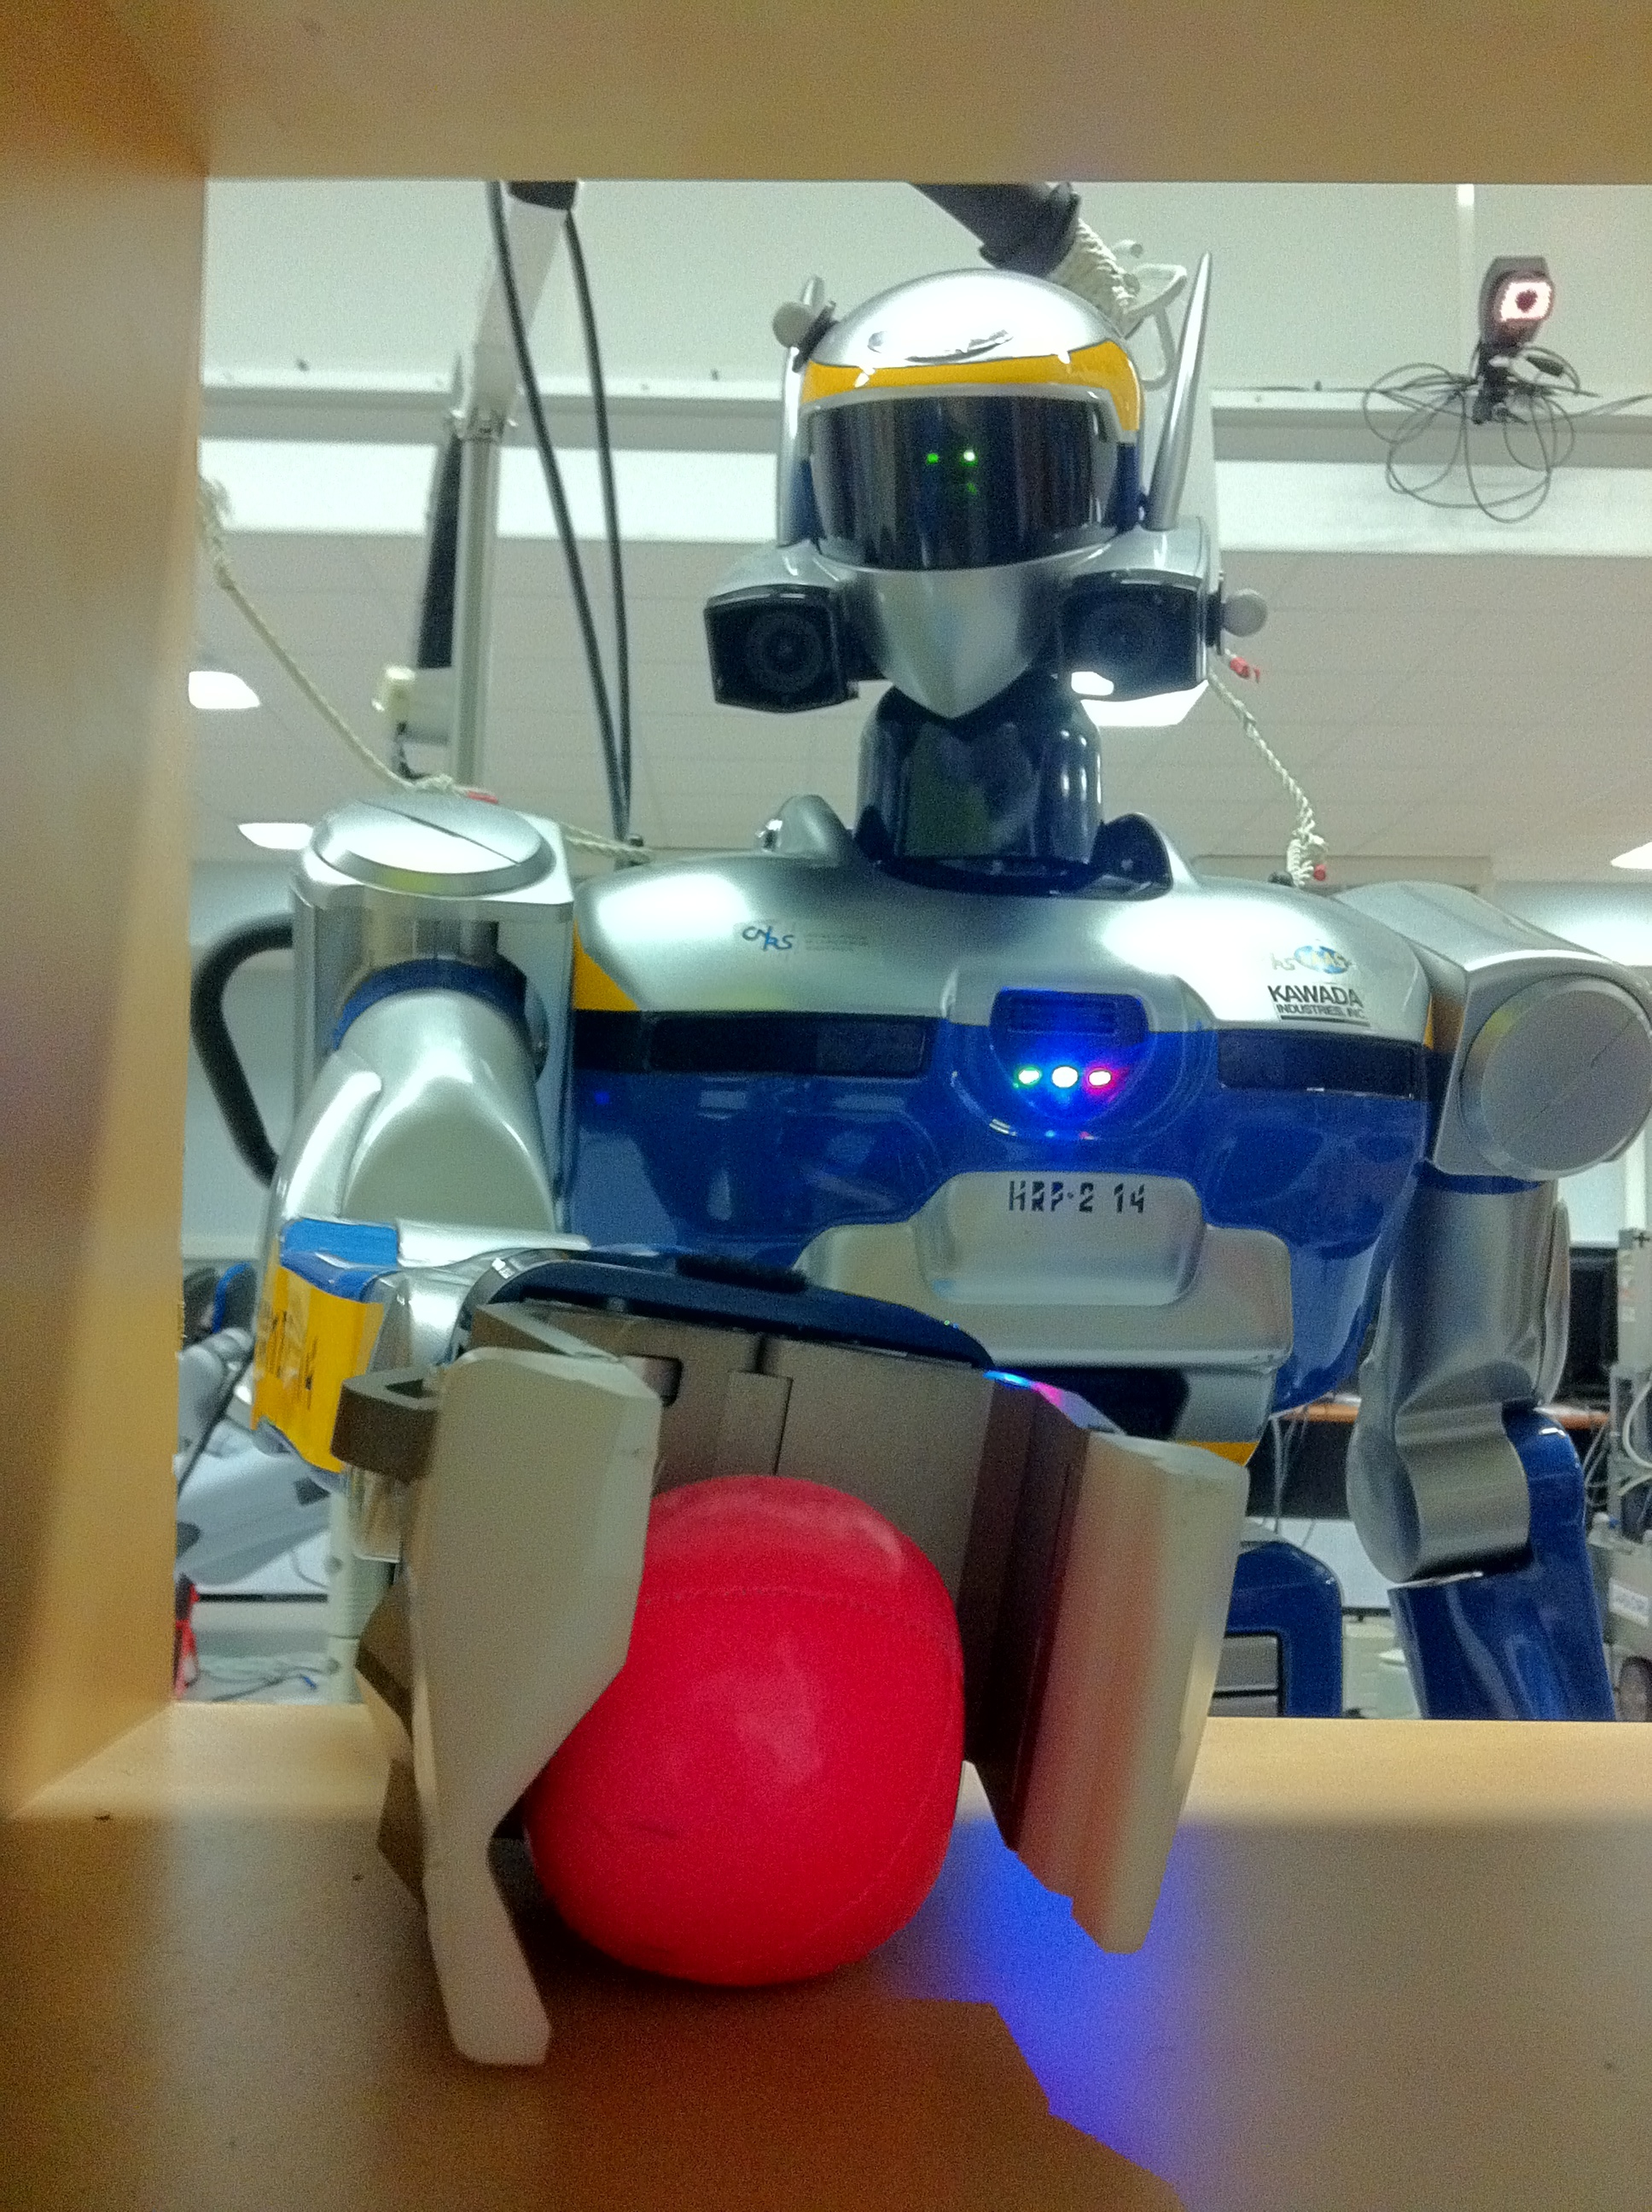
\includegraphics[width=.95\linewidth]{src/chap3-primitive-mouvement/demo1.jpg}
  \end{center}
  \caption{HRP-2 place une balle dans une étagère (I).}
\end{figure}

\begin{figure}
  \begin{center}
    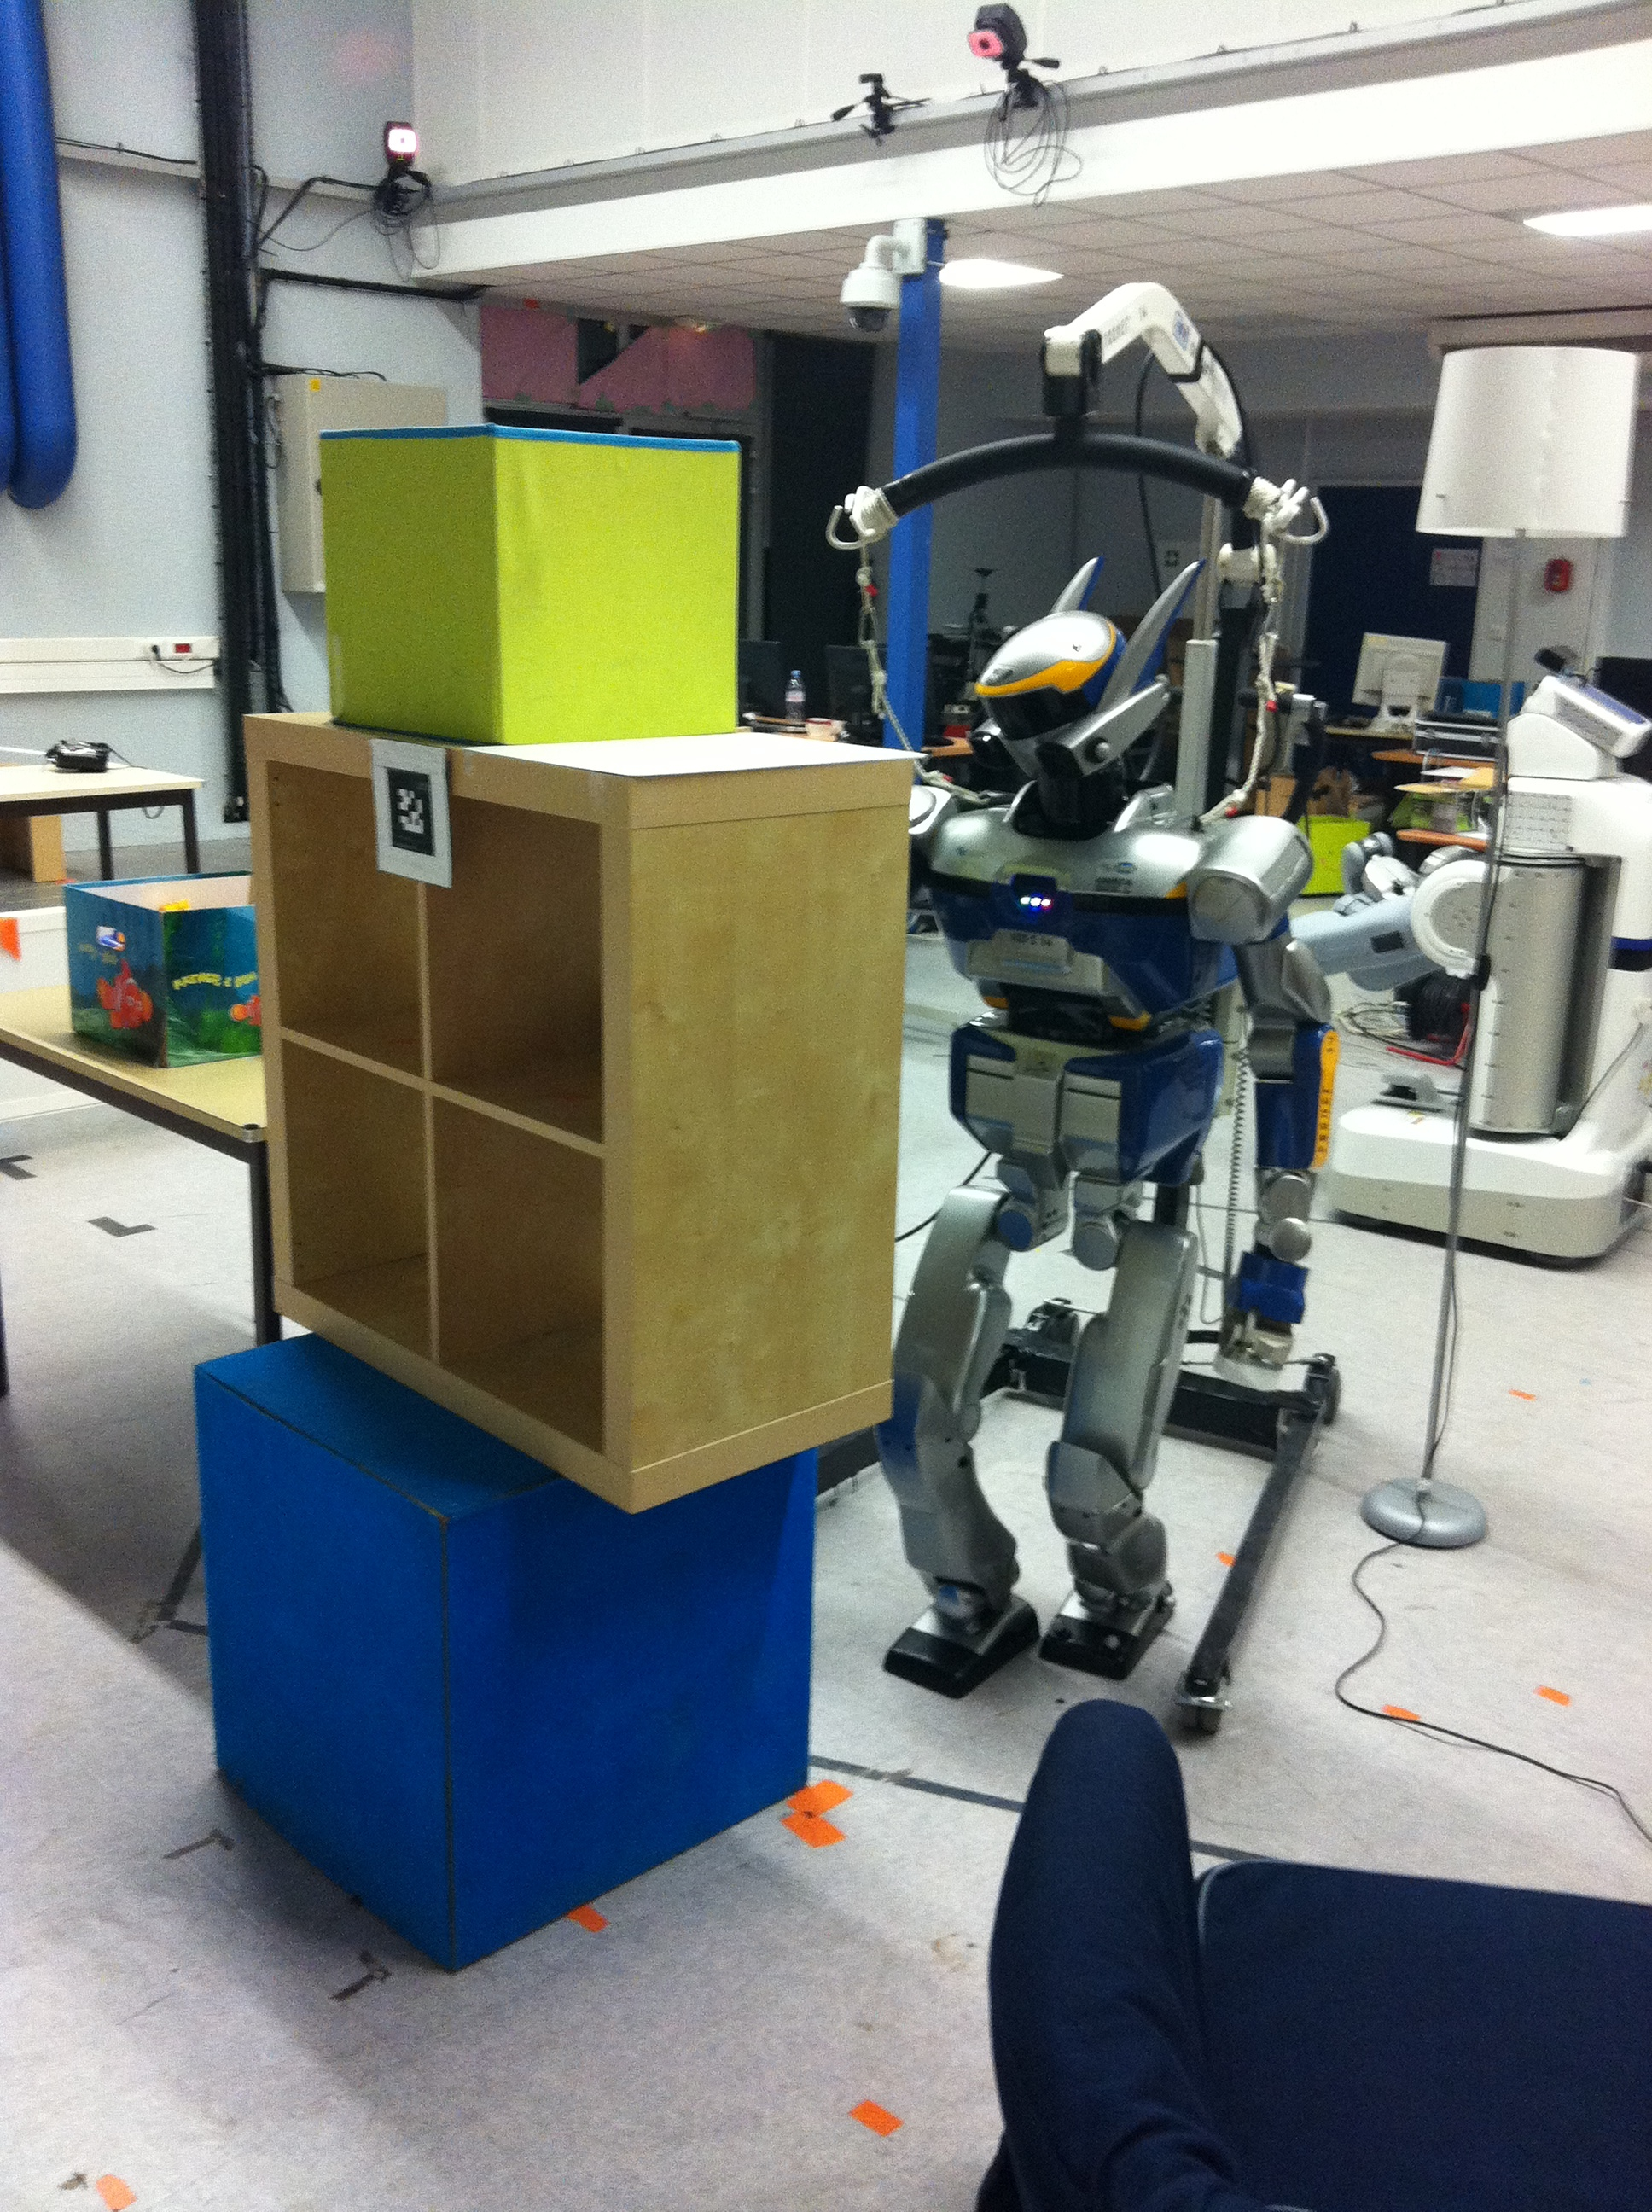
\includegraphics[width=.95\linewidth]{src/chap3-primitive-mouvement/demo2.jpg}
  \end{center}
  \caption{HRP-2 place une balle dans une étagère (II).}
\end{figure}


\begin{figure}
  \begin{center}
    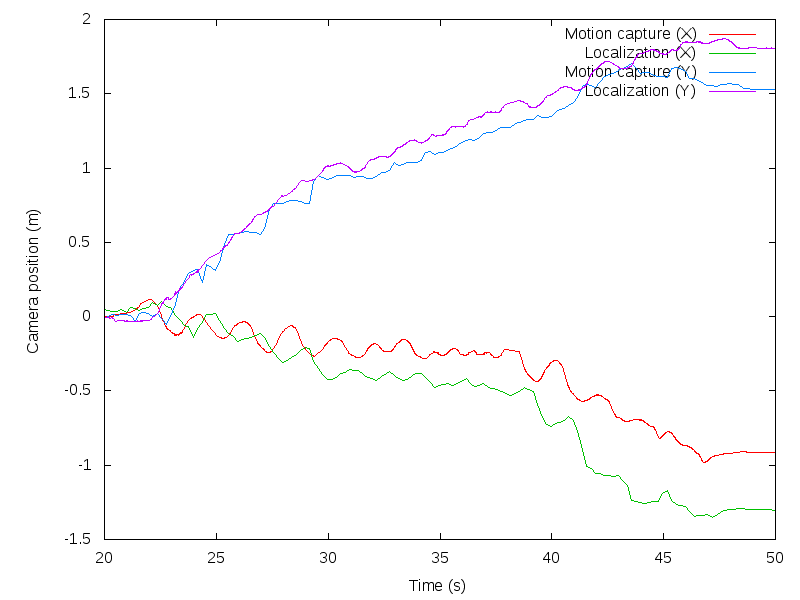
\includegraphics[width=.95\linewidth]{src/chap3-primitive-mouvement/mocap.png}
  \end{center}
  \caption{Précision de l'algorithme de SLAM par rapport au système de
    capture de mouvemement. \label{fig:scenario_visu_precision}}
\end{figure}

\begin{figure}
  \begin{center}
    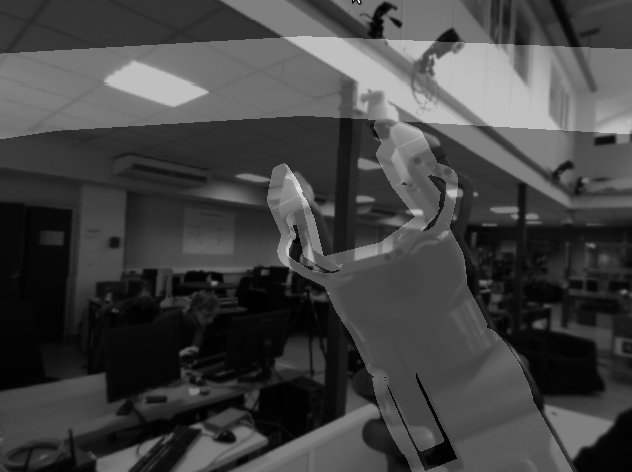
\includegraphics[width=.95\linewidth]{src/chap3-primitive-mouvement/calibextrinsic.jpg}
  \end{center}
  \caption{Reprojection du modèle du robot dans l'image captée par une
    caméra embarquée pour valider la calibration des paramètres de
    cette dernière. \label{fig:reprojection_modele_vision}}
\end{figure}


\section{Conclusion}

Pour continuer à explorer l'expression de plans de mouvement, il
faudrait donc intégrer de nouveaux algorithmes de localisation dédiés
à l'asservissement d'une tâche spécifique plutôt que d'envisager le
problème comme un bloc unitaire. La seconde partie des travaux reste
d'intégrer directement dans la phase de planification une étape de
planification des asservissements. L'idée est de planifier le
mouvement tel que le robot privilégiera le passage dans des zones où
la qualité de la localisation est maximale. En particulier, la
trajectoire de la tête sera calculée afin de laisser les amers
détectables le plus longtemps possible utilisables. Ce planificateur
pourra alors générer la partie asservissement du plan de mouvement
automatiquement. L'intégration de ces deux éléments reste un objectif
clé afin de pouvoir asservir n'importe quel mouvement sur un robot
humanoïde de manière automatique.

%\chapter{Architecture robotique}
\label{chap:integration}

\epigraph{\foreignlanguage{USenglish}{The belief that complex systems
    require armies of designers and programmers is wrong. A system
    that is not understood in its entirety, or at least to a
    significant degree of detail by a single individual, should
    probably not be built.}}{Niklaus Wirth}
\clearpage

\lettrine[lines=2, lraise=0.1, nindent=0em, slope=-.5em]%
{C}{e} chapitre est dédié à la conception d'architectures robotiques
complexes permettant la validation de nouveaux algorithmes robotiques.
Les précédents chapitres ont montré une progression d'une approche qui
est dédiée purement à la génération de trajectoires par l'utilisation
d'outils d'optimisation numérique vers l'exécution de scénarii
dont la complexité a augmentée incrémentalement. Ce passage de la
génération de trajectoire sans ``conscience'' de ce qu'est un système
évoluant dans le monde réel vers une application robotique réelle ne
va pas sans la nécessité d'intégrer et de maîtriser une grande variété
d'algorithmes et de technologies tout en les utilisant conjointement
afin de finalement, atteindre un objectif de haut niveau. Ce chapitre
va donc décrire l'architecture qui a été mise en place sur le robot
humanoïde HRP-2\index{HRP-2} afin de réaliser un ensemble de scénario
expérimentaux, certains faisant partie intégrante des chapitres
précédents et d'autres étant le résultat de travaux de recherche
disjoints, mais prenant appui sur l'architecture développée ici. Ce
chapitre tente également de fournir des conseils et une méthodologie
pour la conception d'applications robotiques.

\section{Architecture}


Les systèmes robotiques peuvent être décomposés en trois grandes
parties:

\begin{enumerate}
\item La couche de perception\index{perception} qui analyse
  l'environnement autour du robot et construit un modèle du monde,
\item La couche de décision\index{décision} qui va tenter de résoudre
  la tâche donnée au système tout en prenant en compte l'état actuel
  du monde,
\item La couche action\index{action} qui va utiliser les capacités du robot pour
  réaliser la tâche proprement dite. En particulier, les capacités
  d'actionnement du robot sont ici utilisées pour impacter le monde
  environnant.
\end{enumerate}


Cette architecture largement décrite par la littérature est encore
d'actualité pour les robots humanoïdes. En effet, cette catégorisation
est issue de la présence dans un système robotique de boucles lentes
et de boucles rapides. Typiquement, la prise de décision est un
processus lent -- qui peut prendre plusieurs secondes --, la
planification de mouvements est un exemple de ce type de processus. Au
contraire, la couche action contrôlant les actionneurs nécessite le
plus souvent d'être extrêmement réactive et impose des contraintes
importantes en terme de temps réel. Il faut pouvoir garantir que la
boucle de contrôle peut être évaluée à une fréquence donnée ce qui
contraint à la fois le type d'algorithmes pouvant être exécuté dans
cette boucle ainsi que le volume de données pouvant être traité. Enfin,
la couche de perception est, elle, en général plus lente que le
contrôle et dépendante de la vitesse à laquelle les capteurs du robot
peuvent fonctionner. Qui plus est, il arrive parfois que les capteurs
acquièrent des données plus vite qu'elles sont traitées et certaines
données sont alors ignorées silencieusement. On a donc ici trois types
de comportements extrêmement différents.


Les couches perception et décision nécessitent une grande puissance de
calcul pour pouvoir assurer une réactivité suffisante. Cette puissance
de calcul est parfois déportée sur un ordinateur spécifique. Par
exemple dans le cadre du robot HRP-2, deux ordinateurs sont
embarqués. Le premier est dédié à la boucle de contrôle temps réel et
est relié aux actionneurs tandis que le second est relié aux capteurs
-- ici les caméras embarquées -- et supporte les algorithmes de
décision et de perception.


Afin de découpler les algorithmes robotiques, chaque algorithme est
implémenté au sein d'un composant robotique\index{composant
  robotique}\index{n\oe ud|see{composant robotique}}. En pratique, un
composant robotique est un processus -- c'est-à-dire un programme
indépendant -- pouvant communiquer avec un ou plusieurs autres
composants. La distribution des calculs sur plusieurs ordinateurs rend
nécessaire la définition d'un protocole de transmission des données
afin de pouvoir assurer une bonne interprétation de ces dernières au
sein d'un environnement informatique hétérogène. Un exemple est la
représentation des nombres au sein des architectures informatiques:
une architecture peut être dit ``big endian''\index{big endian
  (architecture)} ou ``little endian''\index{little endian
  (architecture)} selon l'ordre dans lequel les bits représentants le
nombre sont enregistrés. Dans une architecture ``big endian'' les
bits ayant les poids les plus forts sont contenus en mémoire en
premier tandis que les architectures ``little endian'' adoptent un
ordre inverse. Ce type de problème rend nécessaire la définition d'un
modèle de communication entre composants.


Les architectures robotiques autorisent généralement la communication
entre deux composants, ou n\oe uds, soit sous une forme discrète, soit
sous une forme continue. La forme discrète est appelée
``service''\index{service} et se modélise sous la forme d'un appel de
fonction distant. Un algorithme est généralement divisé en fonctions,
ces dernières formant des blocs logiques pouvant être combinés entre
eux pour réaliser des comportements de plus haut niveau. Les services
fournissent un moyen d'appeler une fonction qui sera non pas exécutée
au sein du processus courant, mais dans un autre processus, voire sur
un autre ordinateur de manière transparente. La difficulté résidant
dans le passage des arguments et la transmission du résultat. Il est
nécessaire que cette fonction soit définie selon des règles
particulières afin de s'asssurer que les données peuvent être
correctement transmises via le réseau sans compromettre leur
intégrité. Cette phase, dite de
``sérialisation''\index{sérialisation}, assure le fonctionnement de
ces mécanismes dans des environnements informatiques hétérogènes. La
seconde forme de communication sert à modéliser des flux de données
continus et est appelée ``topic''\index{topic}. Dans ce cas, le
premier composant communique à un ou plusieurs autres des données
mises à jour régulièrement. De la même façon, un processus de
sérialisation est nécessaire pour assurer que les données peuvent être
transmises même si un ou plusieurs autres composants ne font pas
partie du même processus ou ne sont pas exécutés sur le même
ordinateur.


De nombreux outils logiciels implémentent ces mécanismes sous
différentes formes. Le choix réalisé sur le robot humanoïde HRP-2 a
été d'utiliser ROS -- Robotics Operating System --\index{ROS}, un
projet communautaire initié par la société californienne Willow
Garage\index{Willow Garage}. Le mécanisme de communication ainsi
qu'une grande partie de la modélisation du processus de perception se
fonde sur les outils développés dans le cadre de ce projet. Les
sections suivantes vont détailler les différents composants
fonctionnant sur le robot humanoïde HRP-2\index{HRP-2}.



\subsection{Contrôle}

Sous le terme de ``contrôle'' est désigné le composant robotique
chargé de calculer la commande qui sera envoyée aux actionneurs. Il
est impératif que cet ordre déterminant le prochain état que les
servomoteurs du système vont s'efforcer d'atteindre soit envoyé à une
fréquence fixe. Sur le robot humanoïde HRP-2\index{HRP-2}, la
fréquence de la boucle de contrôle est de 200$\hertz$, il faut donc
que la boucle de contrôle ne mette pas plus de 5ms pour être
évaluée. Les noyaux des systèmes d'exploitation multitâches ne
fournissent pas de garantie forte sur la réactivité des logiciels
exécutés. Il est donc nécessaire d'utiliser des noyaux dédiés afin
d'assurer que la boucle de contrôle soit exécutée en permanence à la
fréquence voulue. Ces contraintes impliquent que les composants de
contrôle se doivent d'être aussi minimaux que possible et sont souvent
monolithiques. À ce sujet, les contrôleurs robotiques partagent une
grande ressemblance avec les noyaux des systèmes d'exploitation. Ils
assurent également la sûreté du système: une mauvaise commande envoyée
aux moteurs peut, très facilement, entraîner la destruction des
actionneurs.

Dans le cas de systèmes robotiques complexes, il est courant d'avoir
plusieurs contrôleurs exécutés successivement au sein de la boucle de
contrôle. Ainsi l'architecture d'HRP-2 se fonde sur un système de
plug-in permettant de charger des contrôleurs ``à chaud''. Chaque
contrôleur est alors modélisé par une machine à état très simple
illustrée par la \autoref{fig:controleur}. Le contrôleur passe alors
par les états suivants:

\begin{itemize}
\item Initialisation sans contrainte de temps réel.
\item Initialisation avec contrainte de temps réel.
\item Exécution.
\item Destruction avec contrainte de temps réel.
\item Destruction sans contrainte de temps réel.
\end{itemize}

\begin{figure}
  \begin{center}
    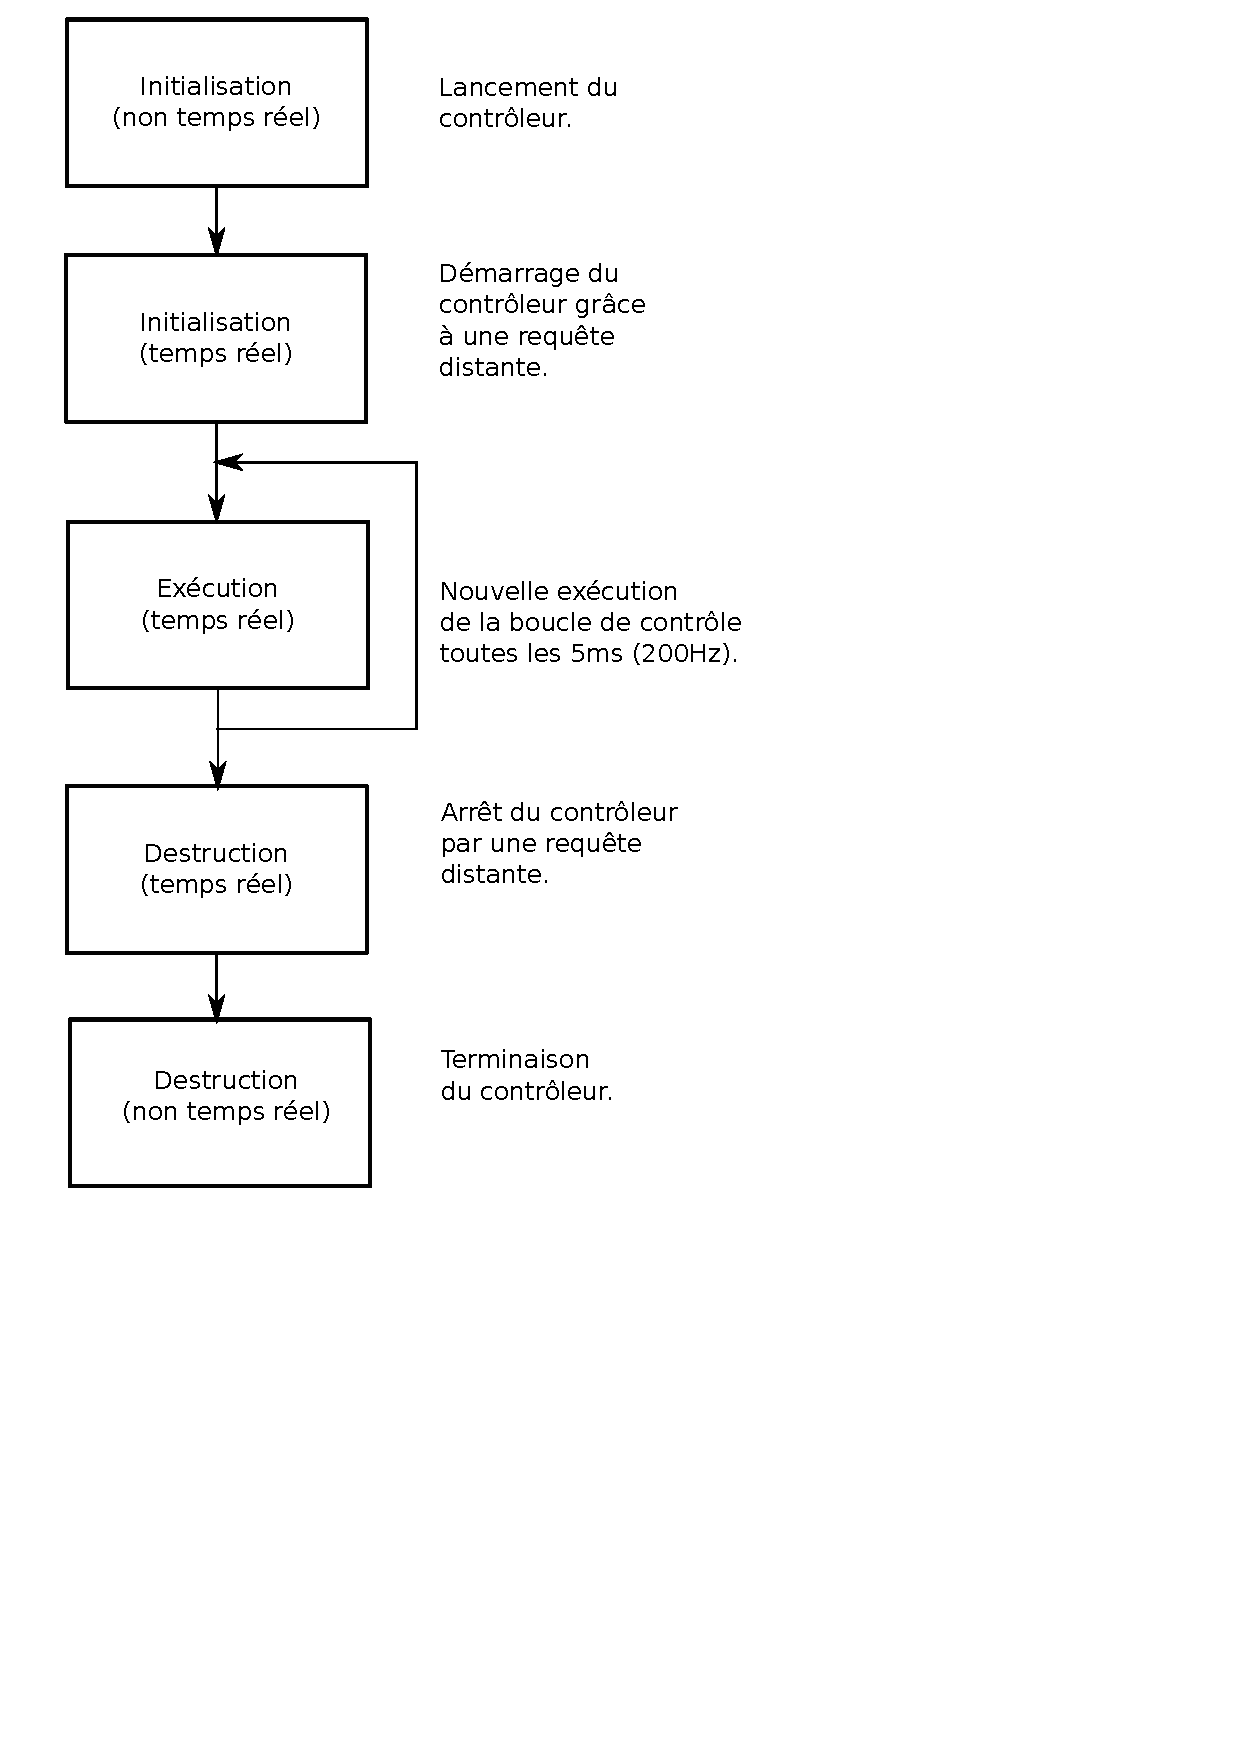
\includegraphics[width=.9\linewidth]{src/chap4-integration/controleur.pdf}
  \end{center}
  \caption{Schéma de fonctionnement d'un contrôleur temps
    réel. Plusieurs contrôleurs de ce type peuvent être lancés. Dans
    ce cas, chaque tour de la boucle de contrôle correspond à une
    exécution de la boucle de contrôle de chaque contrôleur actif --
    initialisé -- dans l'ordre dans lequel ils ont été créés. \label{fig:controleur}}
\end{figure}

Le passage d'un état à l'autre se réalisant dans l'ordre, avec un
bouclage sur la phase d'exécution autant qu'il soit nécessaire.


L'architecture de contrôle est divisée en trois contrôleurs:
\begin{description}
\item[Pile de tâches.\index{pile de tâches}] À partir d'un ensemble de
  tâches, la résolution de la pile de tâches est calculée dans la
  boucle de contrôle afin de calculer la commande à envoyer aux
  moteurs. HRP-2 étant commandé en position, la commande envoyée
  correspond à la position articulaire des différents articulations du
  système.
\item[Stabilisateur.\index{stabilisateur}] HRP-2 intègre un mécanisme
  d'absorption passif des chocs appelé ``silent blocs''\index{silent
    block}. Ce système passif intègre au niveau des chevilles une
  compliance difficile à modéliser et à prendre en compte dans le
  calcul de la commande. La centrale inertielle du robot permettant
  d'estimer l'attitude du bassin, le stabilisateur peut déduire
  l'état des flexibilités des chevilles et, à l'aide des capteurs de
  force placés dans les chevilles, réaliser un asservissement
  bas-niveau sur la trajectoire du ZMP\index{Zero-Momentum Point}
  désiré. Ce mécanisme permet de compenser la modélisation sommaire de
  la dynamique réalisée, par exemple, par l'utilisation du modèle
  simplifié du ZMP ainsi que des éventuelles erreurs de modélisation
  de la structure du robot. Ce système compense les erreurs de suivi
  du ZMP en modifiant les valeurs des articulations des jambes du
  robot.
\item[Communication.] Le dernier élément communique vers l'extérieur
  les informations liées au contrôle du robot tel que les commandes
  envoyées, réellement exécutées -- c'est-à-dire après stabilisation
  --, ainsi que les sorties des capteurs tels que la centrale
  inertielle et les capteurs de force placés aux chevilles et poignets
  du robot.
\end{description}


On notera que pour le dernier contrôleur, la communication réseau
étant implémentée en TCP/IP\index{TCP/IP}, il n'est pas possible de
garantir le temps pris par l'envoi des données et il est donc
impossible d'envoyer des données en TCP/IP\index{TCP/IP} sans
compromettre la boucle temps réel. Cette partie est donc divisée en
plusieurs fils d'exécution non bloquants afin de garantir la sûreté du
système. En pratique, chaque ``topic'' permettant la communication de
données vers l'extérieur publie les données dans un fil d'exécution
séparé et non temps réel. Le fil d'exécution\index{fil d'exécution}
temps réel lui tente de copier la donnée vers une variable lue par ce
fil d'exécution. Si ce dernier est en train d'y accéder et qu'elle
n'est pas accessible, un verrou protège l'accès à la ressource et la
publication de la donnée pour ce tour de boucle est ignorée. En
pratique, la communication vers l'extérieur est réalisée à 20$\hertz$. En
moyenne, une donnée sur dix est donc envoyée afin d'éviter d'engorger
le système.


En terme de conception, les composants nécessitant un rafraichissement
à une vitesse supérieure doivent être intégrés à la boucle de
contrôle. Pour les autres données, il faut pouvoir, via le schéma de
calcul, utiliser les informations temporelles attachées aux
données capteur envoyées pour gérer de manière consistante le retard
inhérent à toute donnée provenant d'une architecture distribuée.


\subsection{Vision}


La vision\index{vision robotique} est l'élément central de la
perception sur un robot humanoïde. Elle est caractérisée par une
particularité qui détermine tous les traitements qui lui sont
affectés: les caméras produisent des quantités de données extrêmement
importantes. De ce fait, il est important d'éviter de réaliser des
traitements inutiles et il faut également éviter au maximum les
copies. Le traitement des images est souvent réalisé en série: on
acquiert une image, on la convertit, on la rectifie et puis on cherche
à en tirer des informations de plus haut niveau. Ces traitements en
série se modélisent particulièrement bien sous la forme d'un tuyau
dans lequel les images passent les unes après les autres. La stratégie
classique de la robotique tend alors à dédier un composant par
traitement afin de garder un système modulaire, mais la taille des
données rend cela difficile. En effet, si chaque composant vit dans un
processus différent, il est nécessaire de passer par des mécanismes de
mémoire partagée afin d'éviter les copies en mémoire. ROS a choisi une
seconde stratégie en offrant la possibilité d'agglomérer plusieurs
composants dans un seul processus\footnote{L'agrégation de plusieurs
  n\oe uds se nomme ``nodelet'':
  \url{http://ros.org/wiki/nodelet}.}. La sérialisation devient donc
totalement inutile au prix d'une plus grande complexité dans
l'écriture des n\oe uds et d'une forme d'insécurité: si un problème
advient dans n'importe lequel de ces composants, il provoquera l'arrêt
de la totalité du système. Cependant, les traitements étant effectués
en série, devoir relancer tous les traitements en cas de panne n'amène
pas de perte significative de qualité de service.


Nous allons donc désormais nous attacher à développer les différents
composants de vision qui ont été utilisés sur le robot
HRP-2\index{HRP-2} et agglomérés dans la chaîne de traitement des
images du robot.


\paragraph{Acquisition des images}

L'acquisition des images est réalisée par un composant communiquant
avec le pilote FireWire. Les quatre caméras du robot sont des Flea2 du
fabricant PointGrey. Ces caméras sont reliées à un FireWire IEEE
1394b\index{FireWire IEEE 1394b}. Les limitations du bus ne permettent
pas l'acquisition des données sur les quatre caméras simultanément, on
peut donc passer de la paire de caméras grand-angle à la seconde paire
de caméras. La première paire est dédiée à la perception de
l'environnement au détriment de la précision tandis que la seconde
dispose d'un champ plus resserré, adapté à la manipulation fine
d'objets notamment.

Les images acquises utilisent un encodage de Bayer\index{Bayer
  (encodage de)}. Cet encodage, nommé du nom de son inventeur, Bryce
E. Bayer chercheur au sein de la société Kodak, réalise l'encodage
d'images couleurs sur 8 bits au lieu des 24 bits habituellement
nécessaires pour représenter les trois canaux utilisés pour encoder
les trois couleurs primaires: rouge, vert et bleu. Cet encodage encode
la couleur verte sur 50\% du volume de données totale tandis que bleu
et rouge représentent 25\% chacun. Cette prépondérance du vert est
fondée sur la plus grande sensibilité au vert des cônes, les
photorécepteurs présents au fond de l'\oe il.


\paragraph{Traitements des images}

Une fois les images acquises, il est important de les convertir dans
un espace colorimétrique\index{espace colorimétrique} adapté à leur
traitement. La première étape est donc de dématricer les images
encodées en Bayer vers des images monochromatiques ou couleurs 24 bits
dans l'espace RGB habituel. Dès maintenant, un branchement s'effectue
entre les traitements utilisant les images couleur et les traitements
utilisant les informations de luminance uniquement. Afin de fournir
une expérience unifiée, les deux ``topics'' sont créés, mais les
traitement ne sont effectués qu'à partir du moment où au moins un
client se connecte à ce dernier. On peut donc offrir une large palette
de possibilités sans mettre à mal les performances du système. Le
dématriçage\index{dématriçage} des images encodées en Bayer
reconstruit les couleurs manquantes en interpolant grâce à la couleur
des pixels adjacents. Plusieurs techniques ayant des coûts de calcul
différents existent selon les cas: interpolation bilinéaire,
interpolation bicubique ou bien encore rééchantillonage de
Lanczos\index{Lanczos (rééchantillonage de)}.


La seconde étape consiste à rectifier les images. Nous nous
intéresserons d'abord au cas de la rectification\index{rectification}
monoculaire. Dans ce cas, l'objectif de ce procédé est de se ramener
au cas de la caméra parfaite dit
``pinhole''\index{sténopé}\index{modèle de caméra
  pinhole|see{sténopé}} -- ou sténopé en français -- où la projection
du point 3D $P$ sur le plan image donne un point 2d $p$ qui correspond
parfaitement à la projection de ce dernier en passant par le point
focal de la caméra $C$: $p_x = P_x / P_z$ et $p_y = P_y / P_z$ où
$P_x, P_y, P_z$ sont les coordonnées du point dans l'espace 3D et
$p_x, p_y$ les coordonnées 2D du point $p$ dans le plan image. Ce
n'est pas jamais totalement le cas en réalité: le plan image n'est pas
un plan parfait, l'axe optique n'est jamais exactement au centre de la
caméra et les objectifs réalisent une distorsion\index{distorsion} des
rayons lumineux captés. Pour pouvoir raisonner sur ce modèle idéal, on
va donc traiter l'image afin qu'elle puisse être considérée comme
provenant d'un capteur idéal ayant le comportement d'un sténopé, à la
différence de la caméra réelle. Il faut pour cela calibrer la caméra
et identifier ses paramètres intrinsèques\index{paramètres
  intrinsèques (de caméra)}: $(u_0, v_0)$ la position de l'axe optique
dans l'image, $(p_x, p_y)$ la taille des pixels permettant de réaliser
la conversion des pixels vers les mètres et un ensemble de paramètres
permettent d'identifier la distorsion de l'image originale. Plusieurs
modèles sont décrits par la littérature, mais dans notre cas une
estimation de la distorsion radiale\index{distorsion radiale} est
suffisante pour compenser l'utilisation d'un objectif grand-angle.


Le processus de calibration\index{calibration (d'une caméra)} est
réalisé en utilisant une mire que l'on place à différents endroits
relativement à la caméra. Connaissant la taille des points et leur
écartement, on peut alors, par la résolution d'un problème type
moindres carrés linéaire, réaliser une estimation des paramètres
intrinsèques des caméras du système.

Une fois de plus, ce traitement est disponible dans deux variantes
différentes: monochromatique et couleur.

\begin{figure}
  \begin{center}
    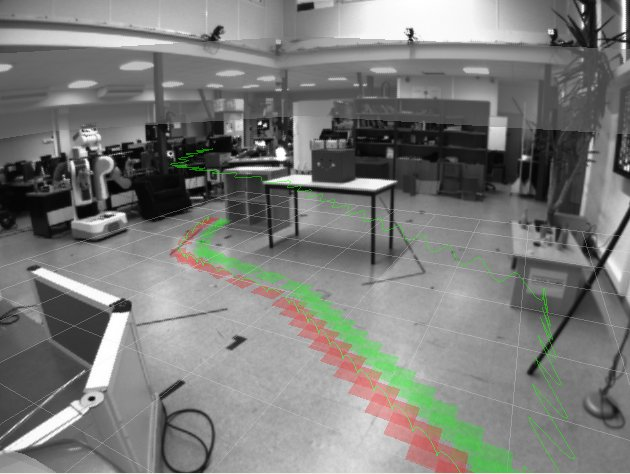
\includegraphics[width=.95\linewidth]{src/chap4-integration/footsteps2.jpg}
  \end{center}
  \caption{Affichage de la pile de pas que le robot va réaliser en
    réalité augmentée.}
\end{figure}



\paragraph{Vision stéréoscopique}\index{vision stéréoscopique}


Le dernier traitement concernait la vision monoculaire. Il est
courant, en robotique, d'avoir recours à la vision stéréoscopique afin
de pouvoir reconstruire la profondeur d'un objet visible dans les deux
caméras. Il est alors nécessaire d'estimer la transformation relative
entre les deux caméras afin de pouvoir rectifier l'image de la seconde
image de la paire de caméras stéréo. Une fois ce processus effectué,
on peut estimer que les images de deux caméras ont été prises par des
capteurs virtuels dont les plans images sont coplanaires. On peut
alors faire en sorte que la projection d'un point 3D se fasse sur la
même ligne tant sur la caméra de gauche que sur la caméra de
droite. Le problème de l'appariement des points se ramène alors à un
problème unidimensionnel de complexité moindre permettant la
construction d'une carte de profondeur. Cette carte est disponible
sous la forme d'un topic, mais les données de profondeur sont
également disponibles sous la forme d'un nuage de points. Dans ce
dernier, on associe à chaque point la couleur du pixel correspondant
dans l'image. Ce topic est particulièrement utile lorsque l'on
souhaite utiliser des algorithmes de traitements de nuages de
points 3D tels que PCL -- la Point Cloud Library --\index{PCL (Point
  Cloud Library)}.


Une fois de plus, la totalité du processus de vision peut fonctionner
dans un processus unique afin d'éviter les copies. Cette architecture,
également adoptée sur le robot PR2\index{PR2 (robot)} de Willow
Garage, fournit donc un compromis intéressant entre rapidité,
souplesse d'utilisation et modularité.

\begin{figure}
  \begin{center}
    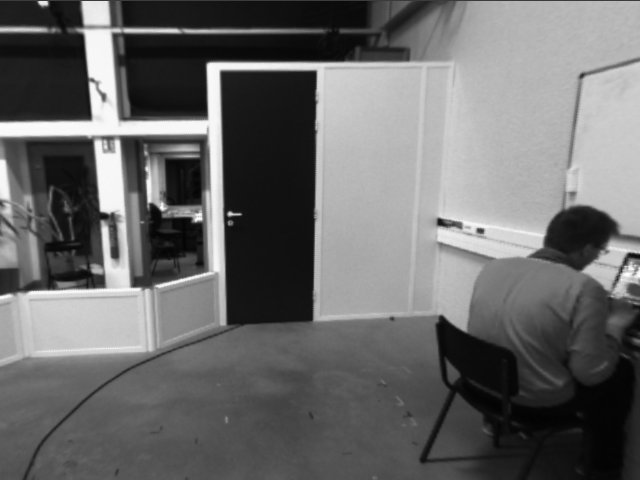
\includegraphics[width=.95\linewidth]{src/chap4-integration/disparity-1.jpg}
    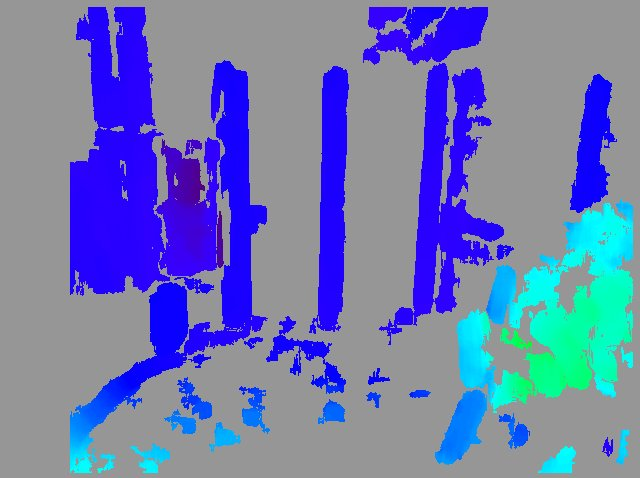
\includegraphics[width=.95\linewidth]{src/chap4-integration/disparity-2.jpg}
  \end{center}
  \caption{Carte de profondeur\index{carte de profondeur} calculée en
    temps réel. Une couleur claire correspond à une faible profondeur,
    une couleur foncée à une profondeur importante. Les zones grises
    indiquent les endroits où aucune correspondance n'a pu être
    établie entre les images de deux caméras. Elles correspondent
    typiquement à une zone peu texturée comme un mur.}
\end{figure}


\begin{figure}
  \begin{center}
    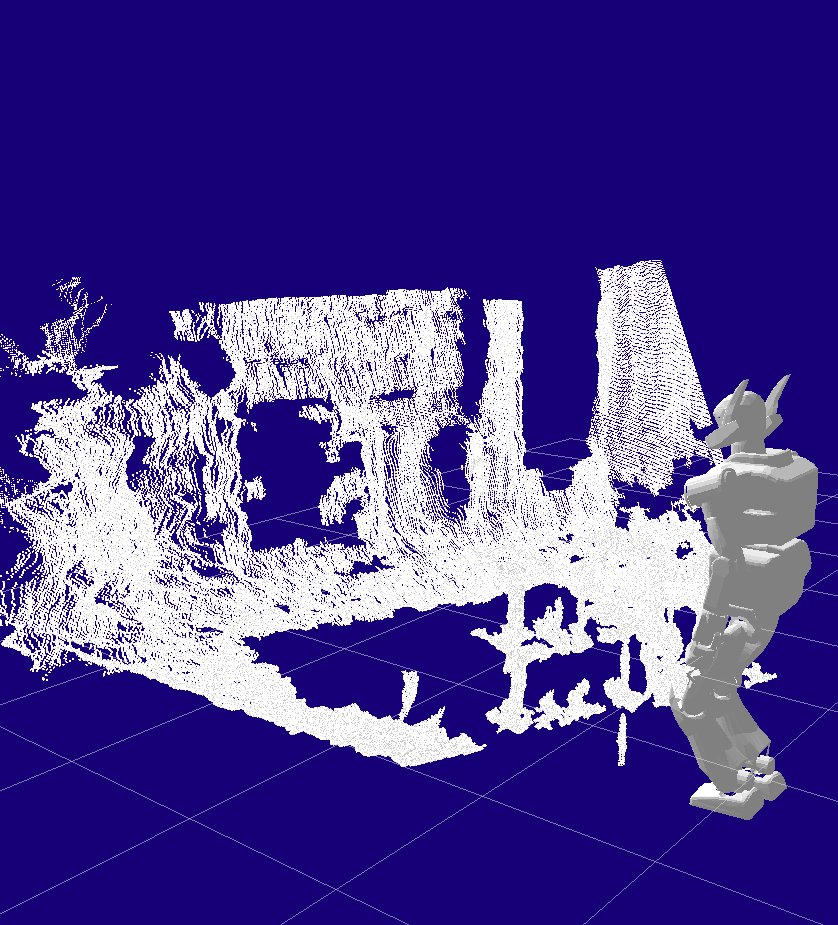
\includegraphics[width=.95\linewidth]{src/chap4-integration/stereo1.jpg}
  \end{center}
  \caption{Reconstruction 3D de l'environnement autour du robot HRP-2
    à partir des données de la paire de caméra stéréo.}
\end{figure}


\subsection{Capture de mouvement}

Une alternative à la vision embarquée est l'utilisation des systèmes
de capture de mouvement. Ces derniers, à l'origine destinés à étudier
les mouvements humains, ont été largement détournés afin de pouvoir
suivre les mouvements d'objets autour du robot et s'abstraire des
difficultés propres à la perception en robotique.


Un composant réalisant l'interface entre d'une part le système de
capture de mouvement et d'autre part l'architecture robotique a été
écrit. Ce dernier permet de suivre les mouvements de plusieurs objets
simultanément et publie une estimation de leur pose via le système de
``topics'' précédemment décrit.


\subsection{Diagnostics et sûreté}

L'utilisation d'un robot humanoïde de grande taille présente toujours
un risque, et ce dernier tend à croître quand l'architecture devient
plus complexe et intègre des composants moins fiables. Pour ce faire,
il est donc nécessaire de pouvoir obtenir un état complet du système
de manière unifiée. Ce dernier est disponible sur le robot et est
illustré par la \autoref{fig:diagnostic}. De plus, il est nécessaire à
tout moment de pouvoir avoir un retour si le mouvement exécuté
présente le risque d'endommager le robot. Ces risques se divisent en
différentes catégories:
\begin{description}
\item[Endommagement des capteurs.] Les capteurs de force sont conçus
  pour résister à un impact de 1000N au plus. Il est recommandé de ne
  pas aller au-delà de 800N par mesure de sécurité. Les autres
  capteurs ne présentent pas de risque particulier.
\item[Endommagement des actionneurs.] Les actionneurs peuvent fournir
  un couple maximal. Au-delà de ce dernier, il risque de chauffer de
  manière trop importante et d'être rendu inopérant. On peut donc
  fixer une borne ``raisonnable'' qui ne devrait jamais être
  dépassée. Évidemment, ceci ne représente qu'une approximation très
  simple des capacités maximums des actionneurs. En particulier, un
  retour sur la température des actionneurs se révélerait être un
  indicateur intéressant, mais n'est malheureusement pas disponible en
  l'état actuel des capacités du robot.
\item[Instabilité lors de la locomotion.] Il est possible d'estimer la
  position du ZMP\index{Zero-Momentum Point} à partir des forces
  mesurées par les capteurs de force. Cette estimation permet
  d'avertir l'utilisateur quand le ZMP se rapproche dangereusement de
  la limite du polygone de sustentation.
\item[Déviation des horloges des ordinateurs embarqués.] Les
  ordinateurs embarqués synchronisent leurs horloges en utilisant le
  protocole NTP -- Network Time Protocol --\index{Network Time
    Protocol (NTP)}. L'ordinateur dédié à la décision et la perception
  se synchronisent sur un serveur de temps distant. L'utilisation d'un
  lien WiFi et la présence de routeurs intermédiaires rendent la
  synchronisation relativement peu précise. Cependant, le problème
  n'est pas très gênant, car le véritable enjeu reste de faire en
  sorte que les deux PCs embarqués gardent leurs deux horloges
  synchronisées. Le lien réseau étant direct, la synchronisation
  relative de ces deux ordinateurs est, au contraire, de très bonne
  qualité et permet d'assurer la cohérence des données temporelles
  entre, d'une part, le contrôleur commandant les actionneurs et,
  d'autre part, les composants de décision et de perception.
\item[Difficultés informatiques d'ordre général.] Au-delà des problèmes
  décrits précédemment et qui affectent plus particulièrement les
  systèmes robotiques, les robots sont également affectés par
  l'ensemble des problèmes qui peuvent toucher un ordinateur:
  température excessive du processeur, manque d'espace de stockage,
  etc.
\end{description}

Une des difficultés de la mise en \oe uvre d'un système robotique est
la nécessité de faire fonctionner un ensemble de technologies sachant
que le mauvais fonctionnement de n'importe quel morceau de
l'architecture peut mettre en péril la tâche tout entière. Qui plus
est, certaines limitations du matériel tel que le couple maximum des
actionneurs sont parfois vérifiées a posteriori. Des systèmes de
surveillance des valeurs critiques sur les couples, les impacts sur
les capteurs de force ont donc été mis en place afin d'éviter
d'endommager le matériel.


\section{Simulation transparente}


Une difficulté récurrente en robotique est la lenteur de la
réalisation des expérimentations: calibrer un robot et réaliser une
expérience demande beaucoup de temps. Afin d'accélérer au maximum le
développement et d'assurer la sécurité des expérimentateurs et du
matériel, une phase de simulation des expérimentations reste cruciale.


L'utilisation d'une architecture robotique fondée sur un modèle de
communication donne ici tout son intérêt: la totalité des capacités du
matériel, tant au niveau de l'actionnement que des capteurs est
représenté informatiquement par un ensemble composé de services et de
``topics''. Tant que le simulateur choisi fournit ce même ensemble de
canaux de communication, les algorithmes pourront fonctionner
indifféremment en simulation ou sur le véritable système. Il reste
alors le plus important: assurer la cohérence entre les capteurs
simulés en fonction des commandes envoyées aux actionneurs. Pour ce
faire, il est important de disposer d'un moteur physique
réaliste. Dans le cadre de cette thèse, le simulateur
OpenHRP\index{OpenHRP (simulateur dynamique)} a été choisi. En effet,
la plupart des simulateurs robotiques -- Gazebo, Webots --, utilisent
des moteurs physiques primitifs adaptés aux robots mobiles ne
réalisant pas de mouvements ``dynamiques''. Afin de modéliser
précisément les interactions entre le pied et le sol, un moteur
physique disposant d'un modèle de contact convaincant et précis est
indispensable à la simulation d'un mouvement réalisé par un robot
humanoïde.


Les limitations de la plate-forme sont généralement liées à la
simulation des caméras, ne pouvant jamais reproduire les difficultés
inhérentes à la vision par ordinateur: changements d'illumination,
délai induit par l'acquisition et le transfert des données, erreur de
calibration de la caméra, etc. La simulation est donc davantage un
moyen de tester la correction du raisonnement et pas tant un outil
fiable pour démontrer sa robustesse à la réalité qui diverge toujours
du modèle calculé.


\section{Modélisation unifiée d'un système robotique}


La génération de mouvement se fonde sur une connaissance précise des
capacités physiques des robots. Cette description est généralement
codée à l'aide d'un format de fichier permettant de représenter les
différentes informations caractérisant le système. Une définition
mathématique du système a été donnée dans le \autoref{chap:suivi}. Du
point de vue informatique, le format de fichier URDF -- Unified Robot
Description Format --\index{Unified Robot Description Format (URDF)},
SRDF -- Semantic Robot Description Format --\index{Semantic Robot
  Description Format (SRDF)} et RCPDF -- Robot Contact Point
Definition Format --\index{Robot Contact Point Description Format
  (RCPDF)} est utilisé pour représenter les informations nécessaires à
la génération de mouvements sur un robot humanoïde. Les deux premiers
formats sont le fruit du travail de la communauté ROS tandis que le
dernier a été développé dans le cadre de cette thèse.

\begin{figure}
  \begin{center}
    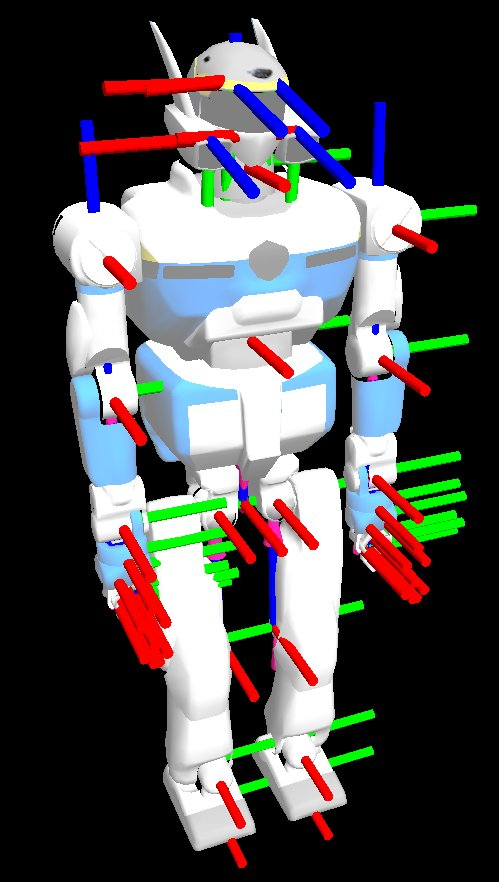
\includegraphics[width=.45\linewidth]{src/chap4-integration/hrp2_urdf.jpg}
  \end{center}
  \caption{Modèle de robot HRP-2 décrit via le format URDF.}
\end{figure}



\subsection{Description d'un robot}


Un robot est un ensemble de corps dont les mouvements relatifs sont
contraints. La modélisation des contraintes passe par la modélisation
des articulations reliant deux corps entre eux. Le format URDF définit
donc deux grands types d'objets: les corps et les articulations. Nous
allons voir quelles informations sont attachées à chaque type d'objet.

\paragraph{Corps}

Un corps est défini par une forme géométrique. Cette forme peut soit
être définie par une primitive géométrique commune -- sphère,
cylindre, boîte -- ou bien via un modèle 3D. Les informations de la
dynamique du corps sont également codées: position du centre de
masse au sein de l'objet ainsi que la matrice d'inertie associée au
corps. Une représentation alternative de la géométrie du corps
utilisée pour les calculs des collisions peut également être
définie. Dans le cas d'HRP-2, une version alternative des modèles des
corps utilisant une approximation convexe avec un pas de dicrétisation
plus grossier est disponible afin de pouvoir accélérer l'évaluation
des collisions. Une version alternative fondée sur l'utilisation de
capsules est également utilisée afin de fournir des tests de collision
rapides pour la planification de mouvements.


\paragraph{Articulation}

Une articulation lie deux corps tout en imposant un ensemble de
contraintes au mouvement relatif de ces deux éléments. Un joint
comporte donc un lien vers le corps ``père'' et le corps ``fils'' pour
définir sa position dans l'arbre cinématique. Dans le cas du joint
racine, il peut ne pas y avoir de corps ``père'' et dans le cas d'un
organe terminal, il peut ne pas y avoir de corps ``fils''.

Les joints supportés sont les suivants:
\begin{description}
\item[Libre.] Ce joint virtuel possède six degrés de liberté et
  n'impose aucune contrainte.
\item[Rotation.] Ce joint possède un degré de liberté unique et impose
  un mouvement de rotation autour d'un axe spécifique au joint.
\item[Translation.] Ce joint possède un degré de liberté unique et
  impose un mouvement de translation le long d'un axe spécifique au
  joint.
\item[Planaire.] Ce joint possède deux degrés de liberté et impose un
  mouvement coplanaire à un plan spécifique au joint.
\item[Fixe.] Ce joint ne possède pas de degré de liberté et impose un
  mouvement rigide entre les deux corps.
\end{description}

Les degrés de liberté des joints possèdent généralement un minimum et
maximum qui sont, soit le résultat de la conception mécanique du joint,
soit lié à la géométrie du robot: une valeur différente entraînerait
immédiatement une autocollision et il n'est donc pas intéressant de
considérer ces valeurs. Chaque joint comporte donc ces valeurs ainsi
qu'une vitesse et une force ou un couple maximum selon le type de
joint. Enfin la friction statique du joint ainsi que l'amortissement
utilisé pour la simulation de ce dernier peuvent également être
enregistrés.


\paragraph{Capteurs}

Une fois l'arbre cinématique défini et annoté par les corps du robot
auquel ils sont attachés, il reste encore un élément clé à spécifier:
la position des capteurs. Pour ce faire, des joints fixes définissent
la position de corps ``virtuels'' sans géométrie permettant de
spécifier la position de points importants du robot tels les capteurs.

Il n'y a malheureusement pas de description générique de ces derniers
qui permettrait de ne pas abuser de la structure cinématique du robot.


\subsection{Modélisation des préhenseurs du robot HRP-2}

La complexité du processus de génération de mouvements pour un système
croît avec le nombre de degrés de liberté. Par exemple,
HRP-2\index{HRP-2} est un système possédant 40 degrés de
liberté\index{degré de liberté}, dont 10 pour les mains. Cependant,
tous ces degrés de liberté ne sont pas commandables. En effet, chaque
main n'est commandée que par un seul degré de liberté décrivant le
niveau de fermeture de la pince. Ces mécanismes sont régulièrement
utilisés dans les robots. On peut également citer le robot Romeo
d'Aldebaran Robotics\footnote{Description officielle du prototype de
  plate-forme: \url{http://projetromeo.com/}} qui s'appuie sur un
mécanisme de commande similaire: un degré de liberté commande
l'actionnement d'une main complète composé de plusieurs degrés de
liberté. Pour modéliser un tel système, il est possible d'insérer des
contraintes et des degrés de liberté ``dépendants'' dans le modèle. On
peut ainsi insérer une contrainte qui va lier deux degrés
ensemble. Par exemple dans la définition du joint A, on peut spécifier
que la valeur du degré de liberté associé dépend de la valeur du degré
de liberté du joint B:

\begin{equation}
  \mathbf{X}_B = \alpha_B \mathbf{X}_A + \beta_B
\end{equation}

Dans l'équation précédente, $\alpha_B$ et $\beta_B$ sont des
constantes propres au joint B. $\mathbf{X}_A$ et $\mathbf{X}_B$ la
valeur du degré de liberté associé respectivement aux joints A et B.


\subsection{Prise en charge des autocollisions}

Une autocollision consiste en la collision de deux corps du
robot. C'est particulièrement facile sur un humanoïde: les bras et les
jambes formant quatre chaînes distinctes pouvant entrer en collision
les unes avec les autres. D'autres cas sont également possibles: par
exemple la jambe de certains robots HRP-2 peut entrer en collision
avec le bassin dans certaines configurations. De manière générale,
toute collision qui requiert le mouvement de plusieurs degrés de
liberté combinés et qui ne peut donc pas être évitée en spécifiant les
bornes des degrés de liberté est une autocollision qui doit être prise
en compte.

Pour déterminer les autocollisions, deux stratégies sont
possibles. L'approche automatique consiste à échantillonner l'espace
des configurations du robot afin de trouver les corps qui sont, soit
toujours en collision, soit jamais en collision. Dans ces deux cas, la
paire de collision est rejetée. Toutes les autres sont ajoutées.  La
seconde stratégie consiste à forger la liste à la main. Dans le cas où
les autocollisions doivent être vérifiées dans la boucle temps réel,
cette technique est souvent utilisée, car les contraintes de temps de
calcul sont trop fortes pour considérer toutes les paires. On se
concentre alors sur les cas les plus probables. En particulier,
certains cas semblent difficiles à détecter automatiquement, notamment
si pour entrer en collision avec le corps A, il faut forcément
traverser le corps B alors il est inutile de prendre en compte le
corps A lors de la vérification des autocollisions.

La liste des paires de collisions est enregistrée dans un fichier
séparé utilisant le format SRDF -- Semantics Robot Description Format
--\index{Semantic Robot Description Format (SRDF)}. Ce fichier stocke
également la position de référence du robot dans lequel il se situe
lors du démarrage des expérimentations.


\subsection{Définition des contacts autorisés}

Un défi ouvert pour la robotique humanoïde dans les prochaines années
est la réalisation de mouvements asservis sur des sols non plans ou
utilisant des contacts avec d'autres zones du corps que les
pieds. Pour un robot donné, les contacts sont autorisés à différents
endroits, typiquement, les mains et les pieds. Il est donc nécessaire
de définir des ``zones'' où les contacts sont autorisés. Cette
information n'était pas formalisée jusqu'à présent dans l'architecture
proposée par ROS et a été le résultat d'un travail réalisé durant
cette thèse. Le format de fichier RCPDF -- Robots Contact Point
Description Format --\index{Robot Contact Point Description Format
  (RCPDF)} associe à chaque corps 0, 1 ou plusieurs zones de
contact. Chaque zone de contact peut être, soit représentée par une
primitive géométrique, soit par un modèle 3D. Les normales du modèles
permettent de définir la direction dans laquelle le contact peut
s'effectuer. Un contact est valide si la force de réaction de
l'environnement sur le corps du robot est colinéaire avec la normale
de la zone de contact mais de direction opposée. Enfin, la force de
réaction maximale en un point autorisée sur cette zone de contact peut
être enregistrée afin d'assurer que le contact ne va pas compromettre
l'intégrité structurelle du robot. Cette représentation offre une
formulation générique qui peut être utilisée pour réaliser des prises
de décisions moins arbitraires que celles qui sont uniquement fondées
sur l'anthropomorphisme. Par exemple, la force applicable sur les
mains du robot peut être plus contrainte ce qui peut pousser un
solveur à faire marcher le robot ``sur ses deux jambes'' sans avoir à
le lui spécifier de manière directe.

En pratique, ces données sont utilisées dans les algorithmes de marche
bipèdes et les systèmes de surveillance afin de calculer les tailles
des semelles du robot -- la zone de contact autorisée sous chaque pied
-- et, de fait, les contraintes auxquelles sont soumises le ZMP.


\subsection{Adaptation du modèle pour le contrôle et la planification}

Instrumenter le modèle pour y incorporer le maximum d'informations est
intéressant, cependant utiliser la chaîne cinématique pour positionner
des capteurs pose des problèmes pratiques. En effet, l'évaluation de
l'arbre est nécessaire pour de nombreux calculs qu'ils soient
géométriques, cinématiques ou dynamiques, inverses ou directs. La
complexité de ces algorithmes est donc dépendante de la taille de
l'arbre et la présence d'articulations, même fixes, pour positionner
les capteurs crée un coût supplémentaire qui semble inutile. Une
proposition est en cours pour modéliser d'une manière plus propre les
capteurs dans le format URDF, mais à l'heure actuelle il semble
intéressant de pouvoir réaliser des simplifications ou ``élagages'' de
l'arbre pour pouvoir en retirer les éléments qui ne sont pas
nécessaires. Dans le cas où les corps que l'on souhaite supprimer sont
des n\oe uds terminaux de l'arbre sans information dynamique -- comme
les capteurs --, alors l'opération peut être réalisée
directement. Cependant, dans tous les autres cas, il est nécessaire de
pouvoir calculer la masse et l'inertie équivalente de l'ensemble des
corps rendus solidaires par la simplification opérée. De fait, ces
transformations de l'arbre sont un moyen bien plus efficace d'exprimer
les contraintes égalités sur certains degrés de liberté que leur
insertion en tant que contrainte dans l'algorithme de génération de
mouvement proprement dit. Les transformations dynamiques de l'arbre
sont également nécessaires pour adapter la géométrie du robot
lorsqu'il est nécessaire, par exemple, de réaliser une tâche de
locomotion en transportant un objet possédant un poids non négligeable
pouvant interférer dans la dynamique du mouvement.

Le système de représentation du robot peut d'ores et déjà coder la
totalité des informations proposées dans cette section, mais il n'a
pas été possible, à l'heure actuelle, d'intégrer le mécanisme de
transformation de l'arbre aux logiciels de planification et de
contrôle utilisés sur le robot humanoïde HRP-2.


\section{Applications robotiques}


L'ensemble des outils décrits dans la section précédente doit être
mis en \oe uvre conjointement afin de pouvoir former une architecture
robotique cohérente. Chaque composant faisant partie d'une
architecture robotique a beau disposer d'un modèle de communication
cohérent, sembler parfaitement fonctionner pris à part et malgré tout
l'assemblage du tout reste une opération délicate: a-t-on suffisamment
de ressources pour faire fonctionner tous les composants à une vitesse
raisonnable? A-t-on une bande passante suffisamment importante entre
les ordinateurs pour communiquer les informations transmises? Le délai
de transmission perturbe-t-il l'architecture? La totalité de ces
questions ajoutées aux difficultés inhérentes au déploiement d'une
application logicielle distribuée nécessite une grande rigueur dans le
développement des démonstrations. Nous allons ici développer un
exemple de scénarii puis montrer quel bilan on peut tirer des séries
d'expériences réalisées durant cette thèse.


\subsection{Mise en place d'une application}


Nous allons présenter dans cette section l'architecture de la
démonstration robotique présentée dans la
\autoref{sec:chap3_localisation}: le robot HRP-2 doit pouvoir réaliser
une tâche de locomotion pour se déplacer jusqu'à un meuble dans lequel
il souhaite déposer un objet -- dans cet exemple une balle rose
--. Pour ce faire, il doit tout d'abord planifier une trajectoire
corps complet, c'est-à-dire combinant à la fois locomotion et
manipulation. Une fois cette trajectoire déterminée, il doit
l'exécuter tout en corrigeant sa trajectoire afin d'atteindre son
but. La localisation est réalisée grâce aux caméras du robot.

Le système est composé des composants robotiques suivant répartis sur
deux ordinateurs -- un pour le contrôle et l'autre pour la décision et
la perception --:
\begin{description}
\item[Ordinateur dédié au contrôle.]
   \\
  \begin{description}
  \item[Contrôle.] Ce n\oe ud est composé d'un solveur fondé sur le
    paradigme de la pile de tâches et d'une infrastructure logicielle
    utlisant le langage de programmation Python pour insérer et
    définir des tâches en cours d'exécution. Les références des tâches
    peuvent être fournies par l'extérieur via des topics. Ce composant
    fonctionne partiellement en temps réel.
  \item[Export des informations capteurs et de la
    commande\footnote{Composant remplacé lors de la simulation par un
      n\oe ud fournissant les mêmes services dans le monde
      simulé.}\addtocounter{footnote}{-1}\addtocounter{Hfootnote}{-1}.]
    La commande envoyée au système, la commande après stabilisation et
    l'état actuel du robot lu sur les encodeurs est publié sous la
    forme de topics. L'accélération linéaire et la vitesse angulaire
    du torse du robot sont également publiés sous la forme d'un
    topic. Ce composant fonctionne partiellement en temps réel.
  \end{description}

\item[Ordinateur dédié à la décision et à la perception.]
   \\
  \begin{description}
  \item[Acquisition des images.\footnotemark] Capture les images venant de la paire
    stéréo grand angle.
  \item[Conversion de l'espace couleur.] Transforme les images encodées
    en Bayer vers des images monochromatiques.
  \item[Rectification.] Corrige la déformation de l'image liée à
    l'utilisation de l'objectif grand angle et à la conception de la
    caméra.
  \item[Localisation.] Réalise une estimation de la position du robot
    dans le monde en utilisant les caméras du robot.
  \item[Cinématique directe.] À partir de l'état des encodeurs, ce
    composant recalcule la position relative de tous les corps et les
    publie sous forme de topics.
  \item[Évaluation de l'erreur de positionnement.] Compare la position
    voulue du robot dans le plan à un instant $t$ à la position perçue
    au même instant.
  \item[Divers.] Plusieurs n\oe uds supplémentaires sont chargés de la
    surveillance des paramètres critiques du robot.
  \end{description}
\end{description}


\begin{sidewaysfigure}[htbp]
  \begin{center}
    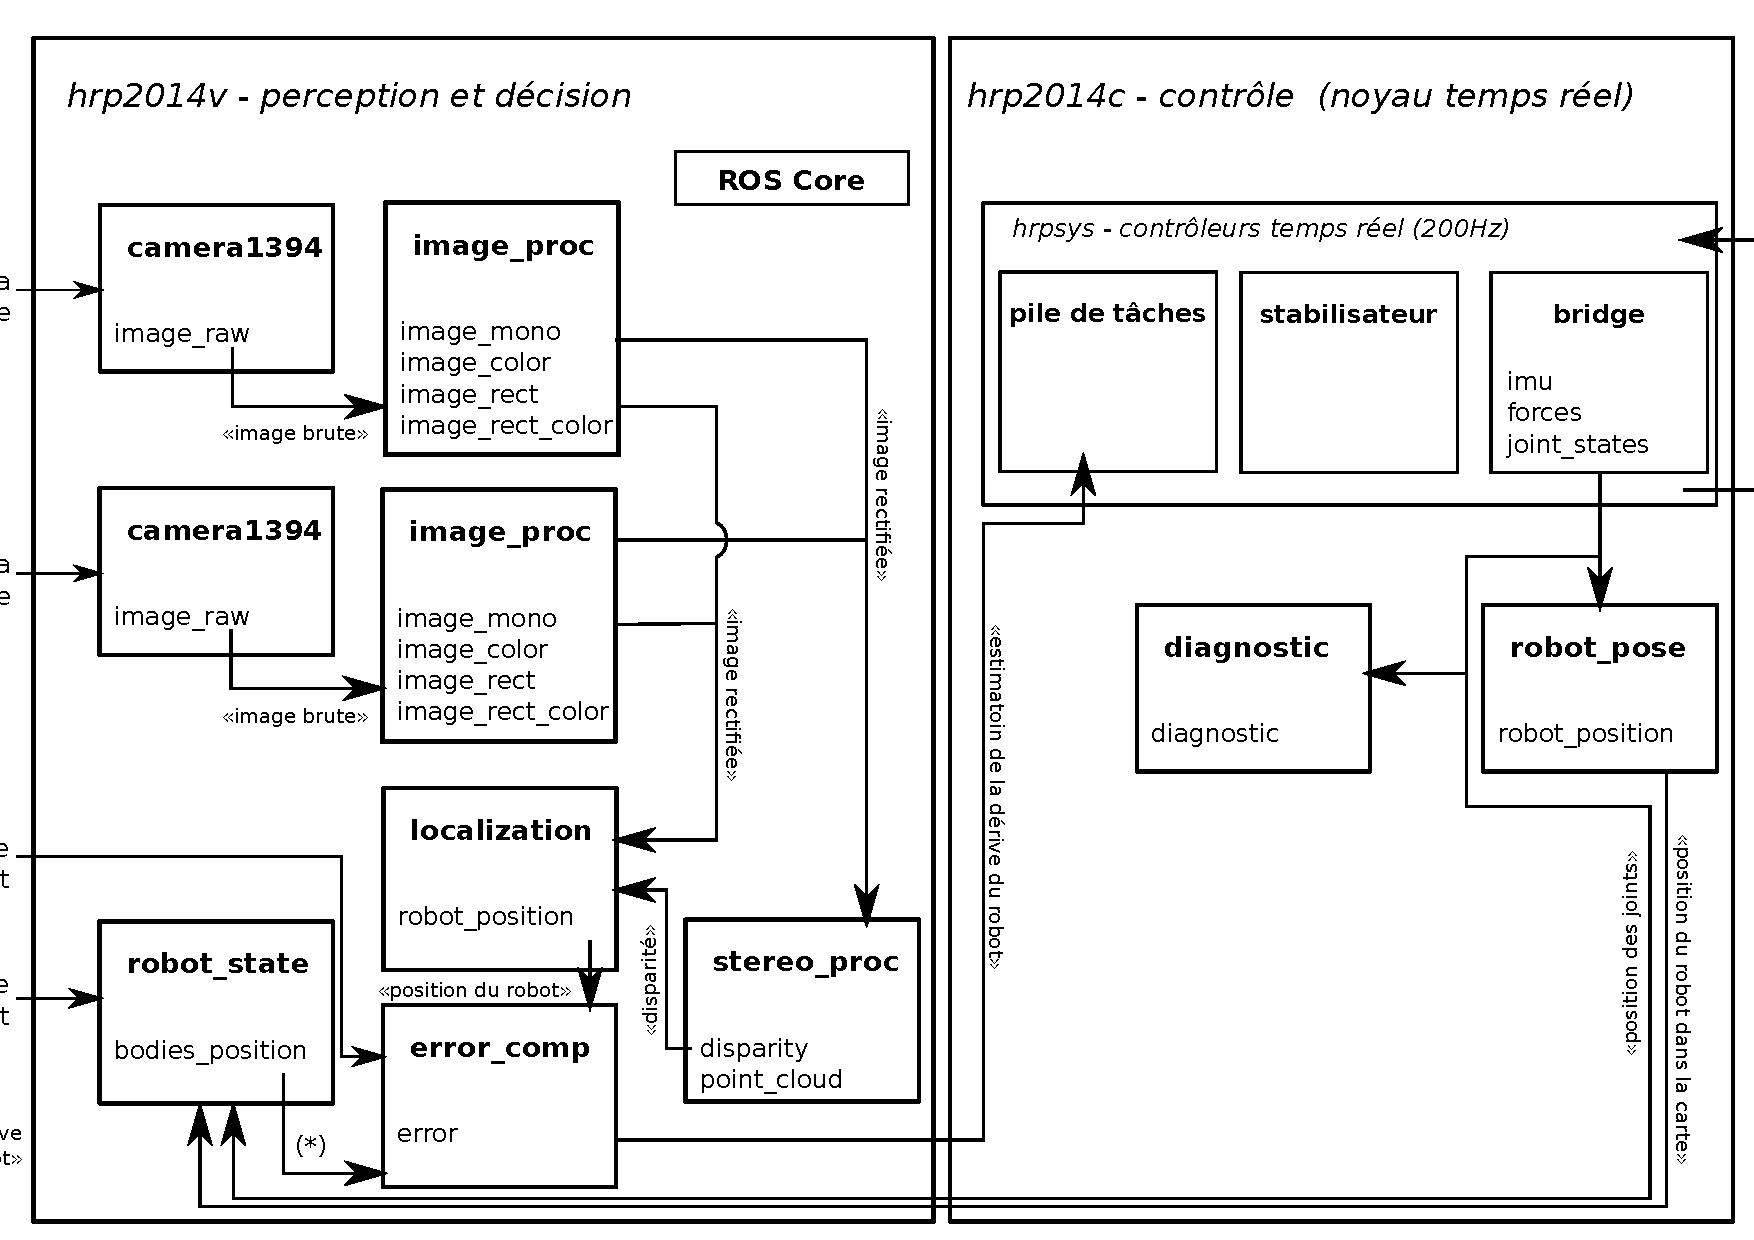
\includegraphics[width=.95\linewidth]{src/chap4-integration/archi.pdf}
  \end{center}
  \caption{Schéma de fonctionnement de
      l'architecture.\label{fig:roscomponents}}
\end{sidewaysfigure}



Ces composants interagissent entre eux et fournissent chacun des flux
de données et des services qui sont détaillés dans la
\autoref{fig:roscomponents}.


Cette architecture a été testée sur le robot humanoïde
HRP-2\index{HRP-2}. L'architecture a fonctionné correctement, mais il
n'a pas été possible d'atteindre une précision suffisante au sein du
système de perception pour compenser avec succès la dérive du
robot. En effet, le SLAM\index{Simultaneous Localization and Mapping
  (SLAM)} tel que configuré ici a donné une précision de plus ou moins
5cm ce qui est insuffisant pour des tâches de locomotions
complexes. On notera également que la phase de planification
n'apparaît pas, elle a été réalisée grâce au travail décrit dans
\cite{11dalibard.humanoids} sous la forme d'un traitement hors
ligne. Le chemin est enregistré sous la forme d'un fichier chargé au
début de l'expérimentation.


\subsection{Difficultés récurrentes}

La mise en place d'une architecture modulaire pour la robotique sert
un objectif principal: contenir la complexité en assurant à
l'utilisateur la possibilité de pouvoir s'abstraire d'une partie des
traitements sous-jacents, quitte à obtenir une solution
sous-optimale. En effet, l'agrégation d'outils aussi différents que la
planification de mouvement, le contrôle, l'asservissement et
différentes techniques de perception nécessite de pouvoir s'appuyer
sur des composants aussi automatiques que possible. En particulier,
concevoir des algorithmes ne nécessitant pas de paramétrage poussé est
important, mais également très difficile. Le paramétrage peut passer,
soit par une phase de calibration -- comme souvent en perception --,
une phase de construction de carte, par exemple pour la navigation --
ou le réglage des stratégies adoptées par les algorithmes. Les outils
de planification nécessitent souvent le réglage de paramètres ce qui
complexifie leur utilisation. Si l'on ne peut paramétrer le système
automatiquement, il faut alors tenter de trouver un ensemble de
paramètres ayant une réalité physique qui puisse permettre à
l'utilisateur de se construire plus facilement un modèle de
comportement de l'algorithme.


Une seconde difficulté concerne l'interprétation des données. La
majorité des algorithmes produisent en sortie des données numériques
possédant un sens physique. Prenons par exemple un composant réalisant
le suivi d'un objet en temps réel: il va alors fournir en sortie la
position de l'objet dans l'espace euclidien 3D. Une ambiguïté se pose
alors: par rapport à quel repère référence cette donnée est-elle
exprimée? La caméra du robot? La racine de sa chaîne cinématique? Un
point fixe du monde? Face aux nombreux dysfonctionnements provoqués
par ce type de problème, ROS\index{ROS} fournit une solution clé en
main: chaque transformation précise, sous forme de chaîne de
caractère, de quel repère à quel repère cette donnée est la
transformation. En enregistrant ces données, on acquiert également la
possibilité de calculer automatiquement des transformations d'un
repère à un autre. Par exemple si l'on fournit la transformation de
$A$ à $B$ et de $B$ à $C$, on peut demander la transformation de $A$ à
$C$ et elle peut être calculée automatiquement. Il y a là un véritable
gain puisque l'on passe d'une implémentation dépendant directement des
données des composants auquel on est lié vers une requête purement
sémantique: ``quelle est la position relative de la cheville gauche
par rapport au poignet droit?''. En réalisant une résolution
automatique des transformations, on se préserve également dans le cas
où les composants utilisés changeraient leur repère de référence entre
deux versions. Une fois de plus, l'absence de typage ici rend le
diagnostic difficile: aucune erreur de compilation n'est possible et
les erreurs dans les valeurs numériques elles-mêmes sont toujours
difficiles à détecter. On notera que le système adopté ici se fonde
sur le traitement des chaînes de caractères ce qui est plus lent que le
recours au typage direct tel que proposé dans \cite{12delaet.ram}.


Une troisième difficulté est la robustesse aux phases
transitoires. Tout système complexe possède une phase d'initialisation
dans laquelle le comportement des modules peut être sous-optimal. En
particulier quand plusieurs composants communiquant ensemble sont
lancés en même temps, il n'y a aucune garantie que le premier
composant terminant son initialisation soit toujours le même. De ce
fait, un composant peut commencer à attendre des données sur un topic
avant que le topic ne soit créé par le premier composant. Le protocole
de communication est extrêmement souple sur ce point et la possibilité
de pouvoir écouter des flux de données qui n'existent pas encore
simplifie de beaucoup le développement en évitant les erreurs lorsque
l'ordre d'initialisation change. Par contre, il est alors nécessaire
de mettre en place, en interne, les mécanismes afin d'éviter les
situations de famine où plusieurs composants s'attendent les uns les
autres indéfiniment. Cependant, le graphe de communication étant le
plus souvent un arbre, ce genre de cas reste peu courant.


La quatrième difficulté concerne l'initialisation du système. Il est
souvent difficile de lancer une démonstration en ``un clic'', mais
plus le nombre d'étapes pour démarrer la démonstration est important,
plus le risque d'introduire une erreur humaine lors d'une
expérimentation augmente. Il est important de limiter les opérations
pour démarrer une démonstration. Un outil utilisé dans le cadre de ce
travail est un formalisme permettant de décrire informatiquement -- en
XML\index{XML} --, le graphe formé par l'ensemble des composants
robotiques ainsi que leurs paramètres respectifs. Ce système réduit
donc au maximum les erreurs humaines, mais certaines difficultés
persistent: un robot humanoïde utilisant une commande à gains forts
telle que HRP-2 s'initialise en l'air, puis il doit être posé, le
système possède donc plusieurs phases transitoires d'initialisation
qu'il est difficile d'automatiser.


\begin{figure}[htbp]
  \begin{center}
    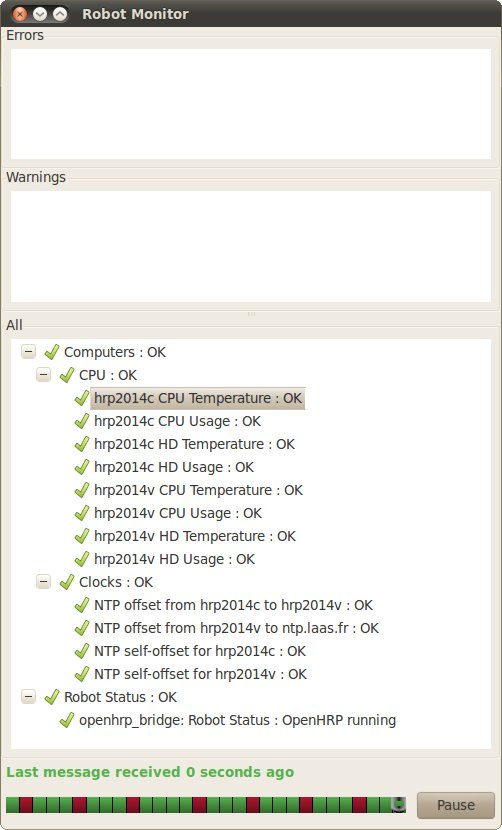
\includegraphics[width=.3\linewidth]{src/chap4-integration/hrp2_diagnostics.jpg}
  \end{center}
  \caption{Visualisation de l'état général du robot fourni par les
    outils de diagnostic automatique.\label{fig:diagnostic}}
\end{figure}



Le dernier problème récurrent est la difficulté pour un utilisateur de
déterminer si le système est dans un état stable et, si ce n'est pas le
cas, arriver à diagnostiquer le système. La section précédente a
développé un ensemble d'outils permettant de surveiller l'état du
robot tant au niveau mécanique, informatique que de l'utilisation qui
en est faite en temps réel -- vérification des couples au niveau des
actionneurs notamment --. Cependant, les problèmes ne viennent pas que
de ces composants ``bas-niveau''. Des composants algorithmiques
peuvent également échouer pour diverses raisons. Pour aider la
compréhension de l'état du système, le premier élément est d'unifier
les mécanismes de rapport d'état. En effet, la plupart des
bibliothèques complexes viennent avec leur système de journalisation
qui n'est pas toujours adapté. Dans le cadre de cette architecture,
nous avons la possibilité de pouvoir agréger les informations dans un
seul topic qui peut ensuite être observé pour connaître l'évolution du
système. On a alors la liste des messages envoyés par les différents
composants dans l'ordre chronologique ce qui n'est pas le cas quand
chacun fonctionne de manière séparée. Les causes et les conséquences
sont, dans ce contexte, bien plus faciles à identifier. Le deuxième
niveau consiste à publier sur le topic de diagnostic l'état du n\oe
ud. Cela correspond à l'un des états suivants: OK, erreur,
avertissement auxquels on associe des données techniques pour aider au
diagnostic, voir \autoref{fig:diagnostic}. Enfin, un service
standardisé peut également être fourni par un composant pour qu'il
tente un autodiagnostic. Ces mécanismes permettent d'aider à la
compréhension des erreurs.



\subsection{Bonnes pratiques pour la robotique}

Cette section détaille la méthodologie à suivre tant pour développer
un composant robotique que pour développer une architecture robotique
complète. Pour développer un composant, un exemple de développement
réalisé pendant cette thèse a été choisi: il s'agit de l'intégration
d'un logiciel de suivi. Le cycle de développement\index{cycle de
  développement} d'une architecture robotique est ensuite détaillé.


\subsubsection{Étude de cas: intégration d'un algorithme de suivi}

Le composant dont il est question ici est librement disponible sur
internet. Il s'agit de la stack ROS\index{ROS}
\texttt{vision\_visp}\footnote{Site officiel:
  \url{http://www.ros.org/wiki/vision_visp}} et plus particulièrement
du paquet \texttt{visp\_tracker}\footnote{Site officiel:
  \url{http://www.ros.org/wiki/visp_tracker}}.


L'algorithme de suivi d'objet a été développé au sein de l'équipe
LAGADIC\footnote{Site de l'équipe LAGADIC:
  \url{http://www.irisa.fr/lagadic/}} -- INRIA Rennes-Bretagne
Atlantique et à l'IRISA--. Cet algorithme utilise l'asservissement
visuel pour calculer une estimation de la pose d'un objet. Le modèle
de l'objet est connu et une estimation initiale de la position de ce
dernier est nécessaire. Une fois cette estimation connue, l'algorithme
tente de minimiser l'écart entre la position des lignes -- bords -- de
l'objet dans l'image par rapport à la reprojection du modèle de
l'objet suivi dans l'image. D'autres critères que les lignes peuvent
être choisis, mais c'est ce dernier point qui a été retenu dans nos
tests. La résolution de ce problème passe par la méthode de
Levenberg-Marquardt\index{Levenberg-Marquardt} qui est proche de
l'algorithme des moindres carrés classiques.


Cet algorithme est partie intégrante de ViSP -- Visual Servoing
Platform -- \footnote{Site du logiciel ViSP:
  \url{http://www.irisa.fr/lagadic/visp/visp.html}}. ViSP intègre
directement des outils pour acquérir des images à partir de caméras ou
lire des données préenregistrées, mais n'est pas un composant
robotique en lui-même.


La première étape a été de concevoir l'interface du composant: flux de données
et services. L'information calculée par ce programme est simple à
définir: il s'agit de la position relative de l'objet suivi par
rapport à la caméra. On peut donc ajouter un repère supplémentaire à
l'annuaire de transformations afin de spécifier la position de l'objet
suivi. Il sera dès lors possible de calculer, par exemple, la position
relative du poignet par rapport à cet objet pour tenter de
l'atteindre, s'il existe une chaîne entre de transformations entre ces
deux repères. En entrée, le problème est plus complexe. Il faut d'une
part un flux d'images, des informations de calibration, un modèle 3D de
l'objet à suivre et un jeu de paramètres permettant de régler
l'algorithme de suivi ainsi qu'une pose initiale.

\begin{figure}
  \begin{center}
    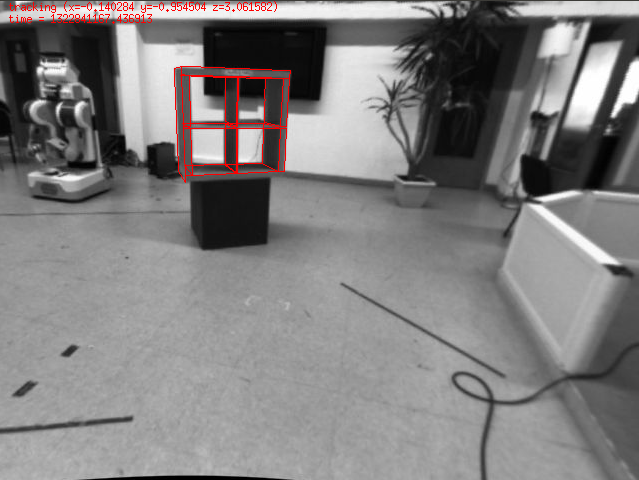
\includegraphics[width=.95\linewidth]{src/chap4-integration/shelf.png}
  \end{center}
  \caption{Le visualisateur associé au composant de suivi d'objet.}
\end{figure}



Il est courant de modéliser le comportement des composants robotiques
sous la forme d'une machine à état. Dans notre cas le composant de
suivi est dans un état ``non initialisé'' au départ où il reçoit déjà
des images et des informations de calibration, mais ne réalise aucun
traitement. Un service permet d'initialiser le suivi en fournissant à
la fois la pose initiale de l'objet, son modèle et les paramètres de
suivi. Le n\oe ud passse alors dans un état actif où il réalise le
suivi. Si le suivi est perdu à un moment ou un autre, le n\oe ud passe
dans un état ``perdu'' où il tente de réinitialiser le suivi avec la
dernière position connue. Si une estimation de la position de la
caméra est disponible, elle va être utilisée pour tenter de fournir
une estimation de la nouvelle position de l'objet en considérant ce
dernier statique. À n'importe quel moment le service d'initialisation
permet de relancer le suivi.


Afin de simplifier l'utilisation du n\oe ud, deux programmes
additionnels sont fournis: le premier permet de calculer une pose
initiale de manière graphique. L'utilisateur peut cliquer sur des
points de l'objet prédéfini et dont on connaît la position relative en
trois dimensions dans l'objet. Cet outil transmet également au
composant de suivi le modèle de l'objet. Le contexte distribué de
l'application empêche de passer directement des emplacements de
fichiers, car il n'y a aucune garantie que le composant réalisant le
suivi et le programme réalisant l'initialisation partage leur système
de fichier. Le modèle est donc directement transmis sous sa
représentation textuelle via le réseau. De plus, le composant pouvant
être lancé à distance, laisser l'utilisateur spécifier le chemin vers
le modèle sous la forme d'un chemin local est une mauvaise idée, car
il sera tenté d'y insérer le chemin sur sa machine et non sur celle où
le composant va être lancé. Pour ce faire, l'emplacement du modèle est
passé sous la forme d'une URI -- Uniform Resource Identifier
-- \citep{rfc2396}.


Le second outil permet de surveiller l'état du tracking en affichant
non seulement la reprojection du modèle dans l'image, mais surtout
l'état du suivi des lignes du modèle. L'algorithme pouvant rejeter des
points pour différentes raisons, cet outil fournit un retour graphique
de ces informations afin d'aider l'utilisateur à trouver le meilleur
ensemble de paramètres pour optimiser le suivi.


Le dernier point à considérer a été d'intégrer le modèle de
calibration de ROS\index{ROS} à ViSP. En effet, ROS annote chaque
image avec les paramètres intrinsèques de caméra\index{paramètres
  intrinsèques (d'une caméra)}. Ces données sont exprimées sous forme
matricielle et doivent être converties avant d'être mises à jour dans
ViSP ce qui nécessite un traitement simple. L'avantage étant que de
cette manière, on peut complètement contourner le processus de
rectification de ViSP qui nécessiterait une calibration spécifique
pour l'utilisation de ce composant.


Les difficultés rencontrées durant cette intégration sont nombreuses:
il a fallu supprimer le code interactif, notamment pour calculer la
pose initiale qui nécessite de cliquer sur une image. Un tel code ne
peut pas fonctionner sur le robot. Il a fallu s'abstraire du système
de fichier local afin de rendre le système facilement distribuable et
il a fallu trouver une façon de pouvoir exprimer les informations de
``debug'' de manière minimale. Une solution aurait été de tracer une
image avec le résultat du suivi, mais les robots étant souvent reliés
en WiFi à la console le contrôlant, transmettre un tel flot
d'information n'est pas justifiable. À la place, un topic
supplémentaire pour les développeur a été ajouté. Le défi est alors
d'assurer la cohérence des données entre d'un côté les images
provenant du composant de vision, de la pose provenant du tracker
ainsi que du topic transportant les informations supplémentaires pour
les développeurs. Ces informations sont filtrées afin que seul les
triplets présentant un temps identique soient affichés. En effet, dans
les précédentes versions, cette synchronisation n'était pas
réalisée. On avait alors l'impression que le suivi était de mauvaise
qualité alors que le problème venait simplement de l'affichage. Les
paramètres de tracking sont également modifiables durant l'exécution
afin de simplifier la recherche du meilleur paramétrage. Cela ouvre
également la possibilité pour un composant de plus haut niveau, de
changer le comportement du logiciel de suivi et réaliser de ce fait,
une forme de suivi ``supervisé''. On notera qu'une fois de plus, la
définition des paramètres joue un rôle très important. Ici l'absence
de sens physique de certains d'entre eux est dommageable: par exemple
la recherche de la nouvelle pose se fait dans un voisinage qui est
défini en pixel. En pratique, cela signifie que si l'on se rapproche
de l'objet, l'absence de reconfiguration de ce paramètre va causer
l'échec du suivi. Un meilleur paramètre aurait été de passer par une
borne sur la vitesse maximum de la caméra qui aurait permis d'avoir un
comportement cohérent quelque soit la distance à l'objet.


Au final, ce composant a reçu un accueil favorable de la communauté
avec plusieurs utilisateurs confirmés dans des laboratoires et
sociétés tiers. Ces utilisateurs n'avaient pas d'expérience avec les
techniques d'asservissement visuel avant de tenter d'intégrer ce
composant et ont réussi à obtenir des résultats satisfaisants dans le
cadre de leur utilisation sur des robots différents, notamment le robot
REEM de Pal Robotics\footnote{Site officiel:
  \url{http://www.pal-robotics.com/}}. De ce fait l'objectif qui
consistait à pouvoir maîtriser la complexité de la mise en place d'un
tel mécanisme a été rempli au travers des choix réalisés ici. Ce
composant a pu être utilisé dans le cadre d'une architecture robotique
distribuée sur deux ordinateurs et l'introduction d'une interface au
niveau de la componentisation robotique a permis au robot HRP-2 de se
localiser, soit en utilisant ce composant, soit en utilisant un
composant de localisation utilisant des amers visuels, soit encore
le système de capture de mouvement de manière transparente. Seul le
lancement du graphe diffère dans ces trois cas.


\subsubsection{Cycle de développement d'une architecture}


La section précédente a décrit le développement d'un composant en
particulier, mais concevoir une architecture ne revient pas à
simplement dupliquer cette approche autant de fois qu'il y a de
composants nécessaires. Il faut tout d'abord découper le problème en
composants cohérents, puis assigner ces composants à un ordinateur
parmi ceux qui équipent le robot et enfin paramétrer chacun des
composants de manière optimale. Dans la mesure où une approche
modulaire a pour intérêt principal la réutilisabilité des composants,
on sera donc contraint par l'interface des composants préexistants que
l'on devra réutiliser, ainsi que par les contraintes matérielles de la
plate-forme: les caméras d'HRP-2 sont connectées à un PC donné donc le
composant d'acquisition des images ne peut fonctionner que sur ce
dernier. Inversement, les commandes sont envoyées via une carte
connectée au second PC, le composant de contrôle ne pourra tourner que
sur celui-ci. De plus, le temps réel contraint le contrôleur a n'être
constitué que d'un seul processus. Le dernier élément à prendre en
compte est la communication intra-n\oe uds: les communications par
``topics'' ou service induisent un retard qui doit pouvoir être
accepté ou géré convenablement. Un autre élément à prendre en compte
est la bande-passante disponible entre les ordinateurs qui constituent
le robot. Il faut s'efforcer de minimiser la bande passante consommée
entre les ordinateurs. Pour les composants effectuant de l'affichage
ou de la surveillance distant le problème est souvent encore plus
critique dans la mesure où le robot est la plupart du temps connecté
en wi-fi et dispose donc d'un lien avec une bande-passante extrêmement
limitée vers l'extérieur. Cela va donc contraindre les
composants de perception, la plupart du temps gros producteurs et
consommateurs de donnée, à se situer sur le même hôte. Une fois le
traitement des images terminé, le résultat final peut représenter un
volume d'informations bien plus compact: trajectoire ou position 3D par
exemple.


En considérant la répartition des composants sur les différentes
machines, il faut déterminer la liste des composants nécessaires. En
général, on part d'un côté de la liste des capteurs que l'on souhaite
utiliser, que l'on fait communiquer avec les algorithmes utilisant ces
données en entrée qui eux-mêmes communiquent avec la partie
décisionnelle. Cette partie étant généralement algorithmique, le
positionnement de ces composants n'est pas soumis à des contraintes
techniques fortes. Enfin, un composant de contrôle est nécessaire pour
envoyer les commandes.


Une fois les n\oe uds choisis et paramétrés, l'étape suivante est la
simulation. De nombreux outils permettent de simuler un mouvement
dynamique dans un monde virtuel. Il est nécessaire ici de remplacer
les composants réalisant l'acquisition des données capteurs par des
composants accédants aux informations équivalentes simulées et le
contrôleur par un contrôleur envoyant sa commande au simulateur. Une
phase supplémentaire de définition du monde est souvent nécessaire.


%\begin{figure}[htbp]
%  \begin{center}
%    %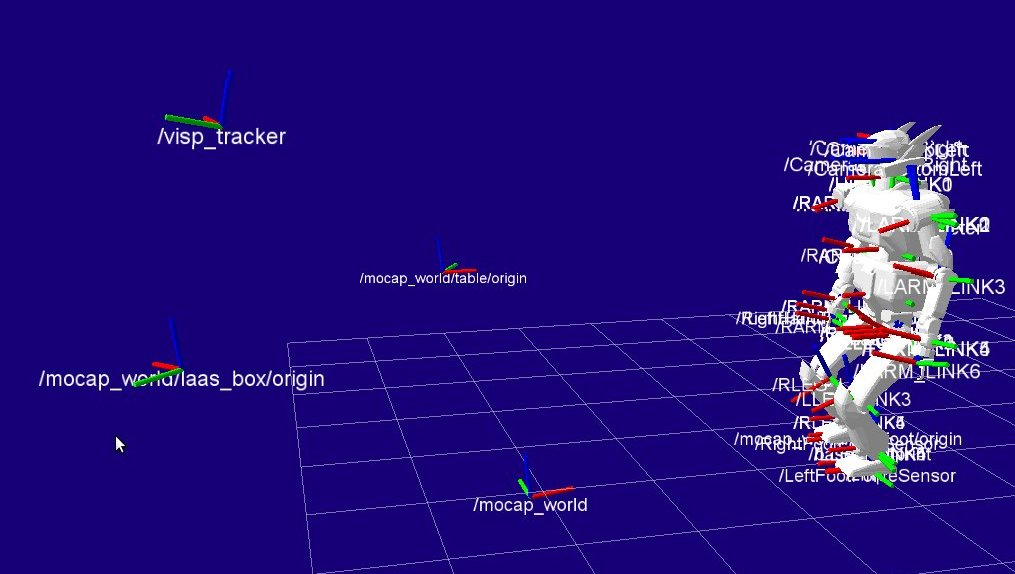
\includegraphics[width=.95\linewidth]{src/chap4-integration/rviz-full.jpg}
%    FIXME
%  \end{center}
%  \caption{Cycle de conception d'une architecture robotique. \label{fig:archidesign}}
%\end{figure}


Une fois validée en simulation, l'architecture est portée sur le robot
proprement dit. On peut alors faire tourner l'architecture sans
envoyer réellement les commandes aux actionneurs afin de vérifier
l'accès aux données capteurs, les délais induits par les
communications entre les hôtes, etc. Enfin, l'architecture peut être
testée réellement en validant plusieurs scénarii adaptés de difficulté
croissante. Une fois l'expérience validée, on peut alors changer
certains composants afin de tester de nouvelles stratégies ce qui fait
débuter un nouveau cycle.


\begin{figure}
  \begin{center}
    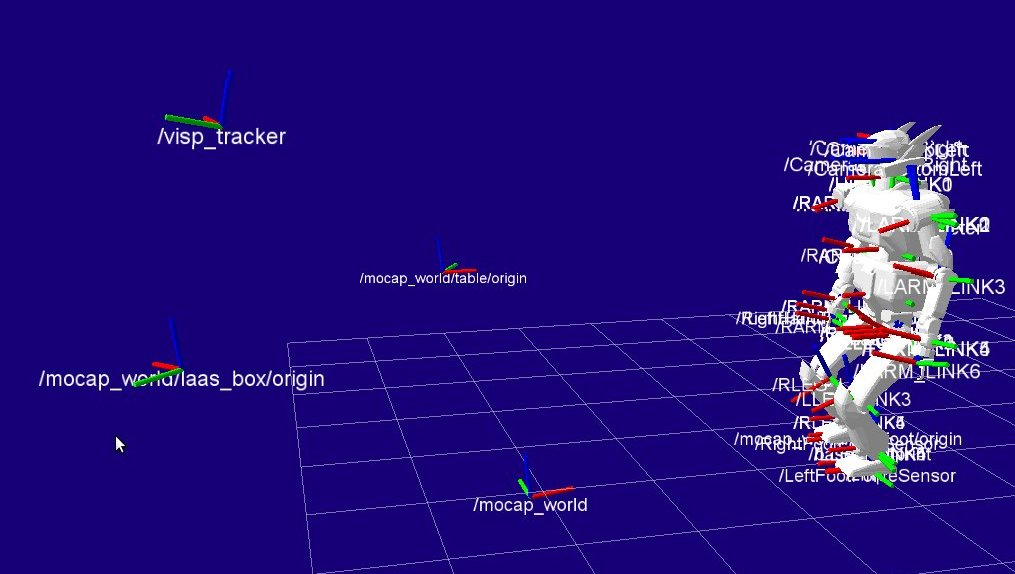
\includegraphics[width=.95\linewidth]{src/chap4-integration/rviz-full.jpg}
  \end{center}
  \caption{Architecture associant de nombreux composants
    robotiques intégrant le contrôleur du robot exécutant une tâche de
    locomotion, le système de capture de mouvement et le processus
    complet de vision utilisant l'algorithme de suivi décrit dans
    cette section pour estimer la position d'un cube.}
\end{figure}



\section{Conclusion}


Construire une architecture robotique est une tâche ardue, non
seulement parce qu'elle agrège des algorithmes complexes, mais surtout
parce qu'il est nécessaire de considérer la plate-forme utilisée et
les problèmes techniques qui lui sont propres -- délais, puissance de
calcul disponible --, afin de construire un ensemble
fonctionnel. Cette section a donc à la fois présenté comment
développer un composant robotique puis comment combiner plusieurs
composants pour réaliser une architecture. Les différentes difficultés
inhérentes à la conception d'un système ont été passées en revue ainsi
que les stratégies qui ont été adoptées au cours de ces trois
années. Il est probable qu'au cours des prochaines années de
nombreuses architectures robotiques voient le jour sur des robots
humanoïdes afin de les rendre sensibles à l'évolution de leur
environnement. Un objectif ambitieux pour lequel les robots mobiles
restent la plate-forme d'expérimentation principale dans l'état actuel
de la littérature.



%\chapter{Conclusion}
\label{chap:conclusion}

\epigraph{\foreignlanguage{USenglish}{Can we actually "know" the
    universe? My God, it's hard enough finding your way around in
    Chinatown.}}{Woody Allen\\\emph{My Philosophy}}
\clearpage

\section{Conclusion}
\subsection{Bilan\ldots}

\lettrine[lines=2, lraise=0.1, nindent=0em, slope=-.5em]%
{L}{es} travaux présentés dans ce manuscrit de thèse ont pour but
d'améliorer les algorithmes de génération et d'exécution de mouvements
pour les robots humanoïdes. Le premier travail présenté a traité de
l'amélioration de la représentation des problèmes d'optimisation afin
de faciliter le prototypage et l'écriture de solveurs, tout en
assurant un haut niveau de sécurité. Un solveur ne doit accepter que
des problèmes qui lui sont adaptés. Une boîte à outils de fonctions de
coût et de contraintes pour l'optimisation de trajectoires a également
été conçue. L'effort théorique principal a été de chercher une
interface telle que la théorie de l'optimisation numérique se trouve
exprimée dans sa totalité tout en excluant les problèmes mal construits
et en maitrisant le coût algorithmique de la résolution des
problèmes. Par exemple, certains gradients ou hessiens peuvent ne pas
être utilisés, mais aucune approximation par différence finie ne peut
être réalisée automatiquement. C'est à l'utilisateur d'explicitement
instancier ce comportement, et d'assumer le coût de calcul
supplémentaire généré par ce type d'approche. Un tel outil est adapté
au post-traitement de trajectoires générées par des algorithmes
aléatoires notamment.

\smallskip

Le second chapitre détaille comment générer une trajectoire de marche
équilibrée sur un sol plan. Les trajectoires sont modélisées sous
forme de tâches et ces dernières sont insérées dans un solveur
temps-réel générant la commande. Le tout forme un contrôleur
polyvalent permettant, entre autres, l'exécution de trajectoires de
marche. Dans des travaux précédents, cette stratégie a déjà été
appliquée pour permettre à un robot humanoïde de marcher mais jusqu'à
présent ces tâches fonctionnaient en boucle ouverte et étaient donc
soumises à une dérive empêchant la réalisation de trajectoires longues
ou nécessitant une grande précision. L'altération du schéma de
contrôle par l'utilisation d'un composant de localisation estimant
cette dérive a permis la réalisation de mouvements d'une grande
précision. La localisation est ici prise en charge par un système de
capture de mouvements.

\smallskip

Cela nous a naturellement amenés à nous poser deux questions abordées
dans le troisième chapitre: peut-on obtenir le même résultat en
utilisant les capteurs embarqués? Peut-on représenter de manière
générique, au-delà de la simple locomotion, des trajectoires
asservies? À la première question, la réponse est, oui, il est
possible de se localiser grâce aux caméras embarquées, mais au prix
d'une précision moindre. Si cette qualité moindre ne gêne pas la
navigation en soi, elle empêche malheureusement toute manipulation
complexe une fois la trajectoire terminée. Il est donc nécessaire de
non seulement asservir la locomotion, mais également la manipulation. La
locomotion nécessite un système de localisation sans dérive, proche
des besoins d'un robot mobile alors que la manipulation nécessite avant
tout un système de localisation dont l'erreur tend vers zéro lors de
la réalisation d'un contact. Un asservissement visuel par exemple est
tout à fait adapté à cet objectif, car plus le robot s'approche de
l'objet, plus la précision croît. Malheureusement, il n'a pas été
possible de tenter une expérimentation intégrant à la fois vision
embarquée, asservissement visuel sur un objet et correction combinée
des trajectoires de locomotion et de manipulation.

\smallskip

Le dernier chapitre, quant à lui, détaille le fonctionnement de
l'architecture robotique mise en place durant cette thèse et qui a été
largement partagée avec d'autres doctorants du groupe. Il est
nécessaire de comprendre le pas franchis puisque l'on est passé d'une
architecture réalisant, soit une lecture des trajectoires articulaires
en boucle ouverte, soit la réalisation d'une pile de tâches avec un
asservissement \emph{ad hoc} dédié au scénario et difficile à
généraliser vers un système fondé sur un ensemble de composants
robotiques réutilisables. S'il n'y a pas eu écriture des composants
robotique, un travail de conception de l'architecture a été nécessaire
afin de permettre l'utilisation conjointe de toutes les capacités du
robot.



\subsection{\ldots et perspectives}


Dans le cadre du travail réalisé pour la modélisation générique des
problèmes d'optimisation, il reste encore de nombreux travaux à mener
dans trois directions différentes. La première est la représentation
informatique de fonctions mathématiques afin d'étendre l'expressivité
des fonctions. L'écriture de fonctions dépendant de plus d'une
variable se trouve compliquée par la nécessité de pouvoir calculer les
gradients combinés issus de la dérivation de plusieurs variables
différentes. La représentation d'espaces mathématiques spécifiques tel
que le groupe spécial Euclidien $\text{SE}(n)$ imposant des
contraintes tacites au solveur. La seconde direction est l'écriture de
nouvelles fonctions afin de pouvoir fournir une boîte à outils plus
complète: optimisation de posture, optimisation de trajectoires
dynamiques, ajout de critères de stabilité tel que le ZMP, etc. La
dernière direction de recherche est l'intégration de nouveaux solveurs
et de nouvelle formulations de problèmes. Par exemple, l'utilisation
du contrôle optimal est très courante en robotique. Ce domaine traite
des fonctions de coût dont la forme est très contrainte et est donc un
intéressant candidat pour être modélisé par le paradigme développé
ici.


\begin{figure}[htbp]
  \begin{center}
    \includegraphics[width=\linewidth]{src/chap5-conclusion/darpa.jpg}
  \end{center}
  \caption{Le défi DARPA pour les robots humanoïdes: les robots
    devront, entre autres, remplacer une vanne et détruire un mur pour
    pouvoir y accéder. \label{fig:darpachallenge}}
\end{figure}


Concernant le travail d'exécution de trajectoire sur robots humanoïdes,
le chemin qui reste à parcourir est clair: pour pouvoir asservir une
trajectoire automatiquement, il faut encore valider la correction des
trajectoires de manipulation, ainsi que l'utilisation d'algorithmes de
vision pour estimer la déformation nécessaire de la trajectoire des
bras. Une fois les tâches de locomotion et de manipulation asservies,
il faudra alors prendre en compte ces contraintes dans la phase de
planification. À l'heure actuelle, le planificateur peut générer un
plan de mouvement, mais il ne prend pas en compte la visibilité des
amers dans la phase de génération de la trajectoire. Il faut
privilégier les chemins assurant une qualité maximale de
l'asservissement. Les contraintes imposées par les systèmes de
localisation variant selon les cas, un dialogue entre l'étage de
planification et l'étage de perception et localisation est nécessaire.
La dernière étape serait alors de ne plus se contraindre à des
transitions temporelles dans le plan, mais également insérer des
événements logiques. Pour ce faire, il sera nécessaire d'insérer dans
l'architecture un superviseur de haut niveau permettant de réaliser la
transition entre les états logiques ainsi que de gérer les retours sur
erreur.


En conclusion, les travaux entrepris durant ces trois ans ont permis
de poser les fondations de l'exécution de trajectoires asservies sur
le robot humanoïde HRP-2, mais il reste encore un important effort à
fournir pour arriver à exécuter des scénarii longs et précis de
manière fiable. Il est fort probable que les années à venir voient
d'importants travaux dans ce sens, le prochain défi proposé par la
DARPA\index{DARPA} \citep{12darpa} étant destiné aux robots humanoïdes
-- voire \autoref{fig:darpachallenge} --. Ces derniers devront
réaliser des mouvements complexes tels que monter une échelle ou bien
encore conduire une petite voiture. Les techniques de fermeture de
boucle comme celle qui a été proposée dans ce manuscrit joueront sans
doute un grand rôle dans la réussite de scénarii de ce type.

%
%
\backmatter

\addcontentsline{toc}{chapter}{Liste of figures}
\listoffigures
\addcontentsline{toc}{chapter}{Liste of tables}
\listoftables

%
% Bibliography
\addcontentsline{toc}{chapter}{Bibliography}
\nocite{*}
\bibliography{thesis}
%
% Index
\cleardoublepage
\addcontentsline{toc}{chapter}{Index}
\printindex
%
\end{document}
